\documentclass[a4paper, 11pt]{article} % Papier A4, police 11
\usepackage[margin=2.5cm]{geometry} % Marges de 2.5cm (plus joli)
\usepackage{graphicx}  % Permet d'inclure des images
\usepackage{float} %Pour les legendes des images
\usepackage[T1]{fontenc} % Permet d'utiliser des accents
\usepackage{pdfpages}  % Pour inclure des documents PDF externes
\usepackage{amsmath} % Pour aligner les équations
\usepackage{hyperref} % Pour les liens
\usepackage{multirow}
\usepackage[table]{xcolor} % Pour le fond gris
\usepackage{subcaption} % Pour utiliser les sous-figures
\usepackage{wrapfig} % Pour wrap le text autour des images
\usepackage{microtype} % Rend le document légerment plus joli apparament
\usepackage[none]{hyphenat} % Desactive les tirets qui cassent les mots
\usepackage{tabularx}
\usepackage{array}
\usepackage{listings} % Pour inserer du code
\usepackage{placeins}


% Marges autour des figures
\setlength{\columnsep}{20pt}

% Couleur des liens
\hypersetup{
    colorlinks=true,
    linkcolor=black,
    urlcolor=blue,
    pdftitle={Projet FlyForce - Groupe 1},
}

% Nom de la table des matière
\renewcommand*\contentsname{Table des matières}

% Evite les alinéas en début de paragraphe
\setlength\parindent{0pt}
\setlength\parskip{\medskipamount}

\begin{document}
\begin{titlepage}
    \begin{center}  
        \Huge
        \textbf{Projet FlyForce }\\
        \vspace{0.3cm}
        \textbf {Groupe 01}
        \vspace{1cm}
            
        \normalsize
        \begin{center}
        \begin{tabular}{ c c c }
            Arnaud Campiche    & Martin Tonascia    & Axel Fouet    \\  
            Louka Kachakhidze  & Nestor Guibentif   & Daniel Roulin \\  
         \end{tabular}
         \end{center}
         \vfill

         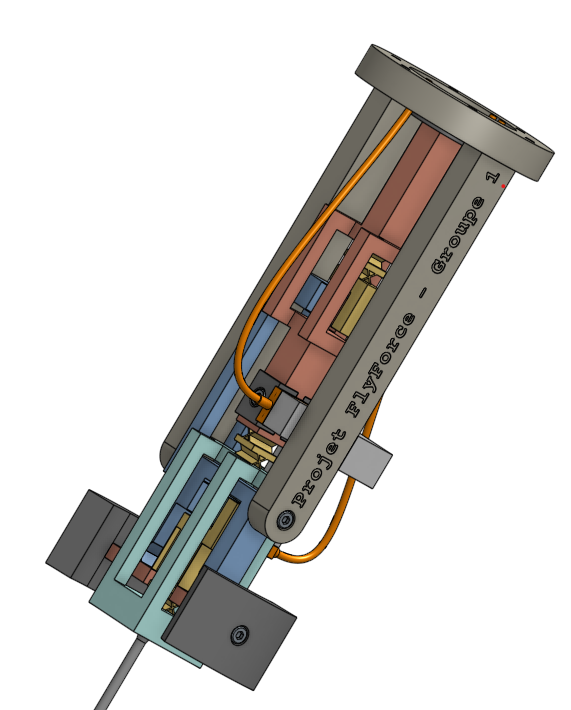
\includegraphics[width=0.7\linewidth]{images/screen_flyforce.png}

         \vfill
            
       Conception de Mécanisme II \\

       \vspace{1cm}

    
\includegraphics[width=0.3\linewidth]{images/logo-epfl.png}

            
    \end{center}
\end{titlepage}
\begingroup
\let\clearpage\relax % évite le saut de page automatique
\scriptsize

\tableofcontents
\endgroup
\newpage
\section{Introduction}
Le projet FlyForce a pour but de concevoir un mécanisme entièrement en guidages flexibles permettant de prendre des mesures de dimensions de pièces mécaniques par palpage, grâce à l'utilisation d'un stylet. Nous avons donc conçu un système qui détecte les forces (±5N selon cahier des charges) appliquées sur le stylet: ce dernier translate selon z et tourne autour des axes x et y (voir section \ref{conceptionito}).
\\Ce rapport décrit premièrement la conception du mécanisme, c'est-à-dire l'idée générale de son fonctionnement, ensuite sont détaillés le dimensionnement et les différents choix de construction et de matériaux, et finalement une discussion des erreurs. Les principales sources théoriques de ce rapport sont l’ouvrage \textit{Conception de guidages flexibles}, de Simon Henein, ainsi que le cours \textit{Conception de mécanismes}. La majorité des formules utilisées pour la modélisation, la conception et le dimensionnement du mécanisme proviennent directement de cet ouvrage et de ce cours, qui ont servi de références tout au long du développement. 

\section{Conception générale}
\label{conceptionito}
\subsection{Explication du principe de fonctionnement}
\subsubsection{Principe de guidage du stylet à 3 degrés-de-liberté}

\begin{figure}[H]
    \centering
    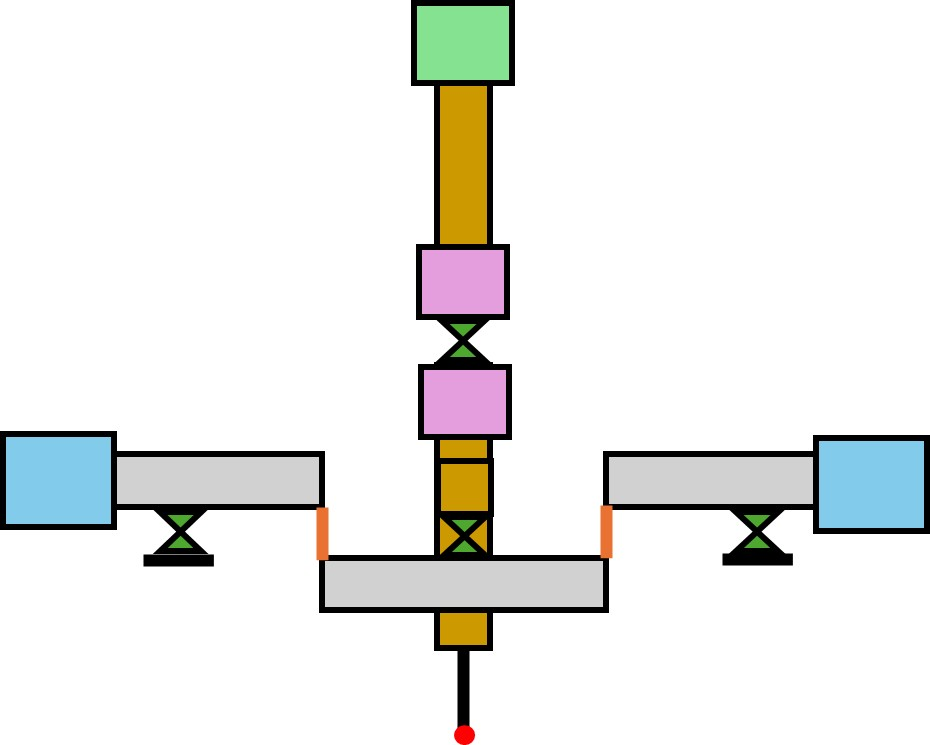
\includegraphics[width=0.35\linewidth]{images/flyforce_neutral.jpg} 
    \caption{Schéma du mécanisme }  
    \label{fig:mouvement_neutre}
\end{figure}
Notre mécanisme est séparé en deux parties. La première est composée des poutres en gris sur le schéma et se charge de l'équilibrage en z. La deuxième comporte les poutre marron et s'occupe de l'équilibrage en x et y.


\subsubsection{Principes d’équilibrage en force et en moment}

L'équilibrage en x et en y se fait de la même manière. Le mouvement du stylet fait tourner une deuxième poutre dans le sens opposé. La masse supérieure en vert permet d'équilibrer en moment et les masses en rose permettent d'équilibrer en force le mécanisme dans ces deux axes.

L'équilibrage en z se fait grâce au deux masses bleu clair fixées aux extrémités. Quand le stylet monte, grâce aux pivots et aux lames fixées sur la partie grise, les masses descendent et inversement.

\begin{figure}[H]
    \centering
    \begin{minipage}[t]{0.30\linewidth}
        \centering
        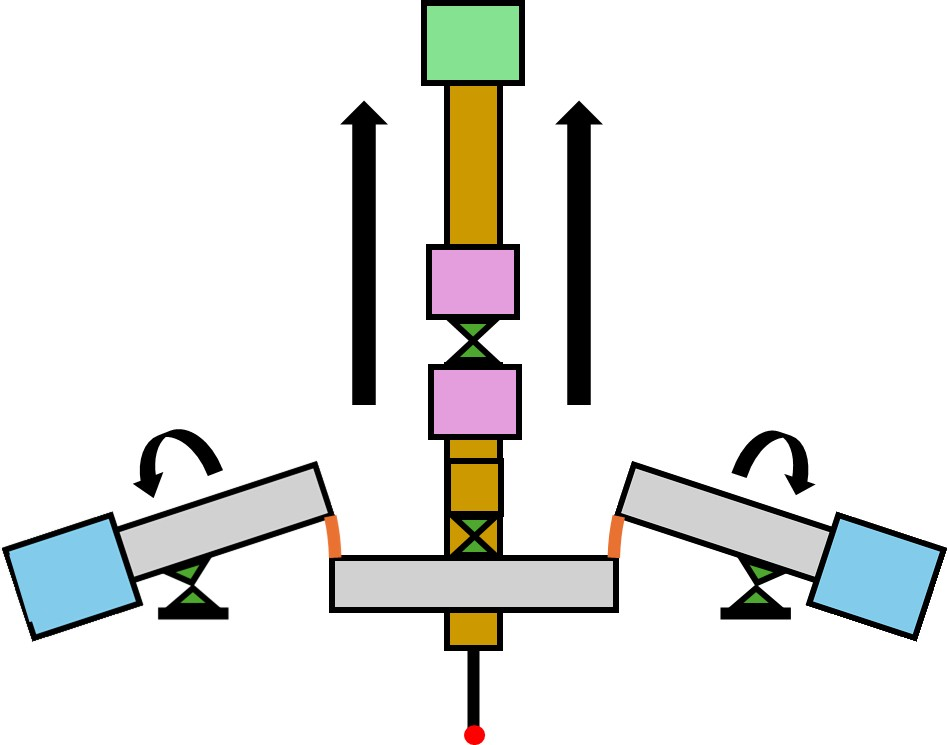
\includegraphics[width=\linewidth]{images/flyforce_z.jpg} 
        \caption{Translation en z}  
        \label{fig:mouvement_z}
    \end{minipage}
    \hfill
    \begin{minipage}[t]{0.30\linewidth}
        \centering
        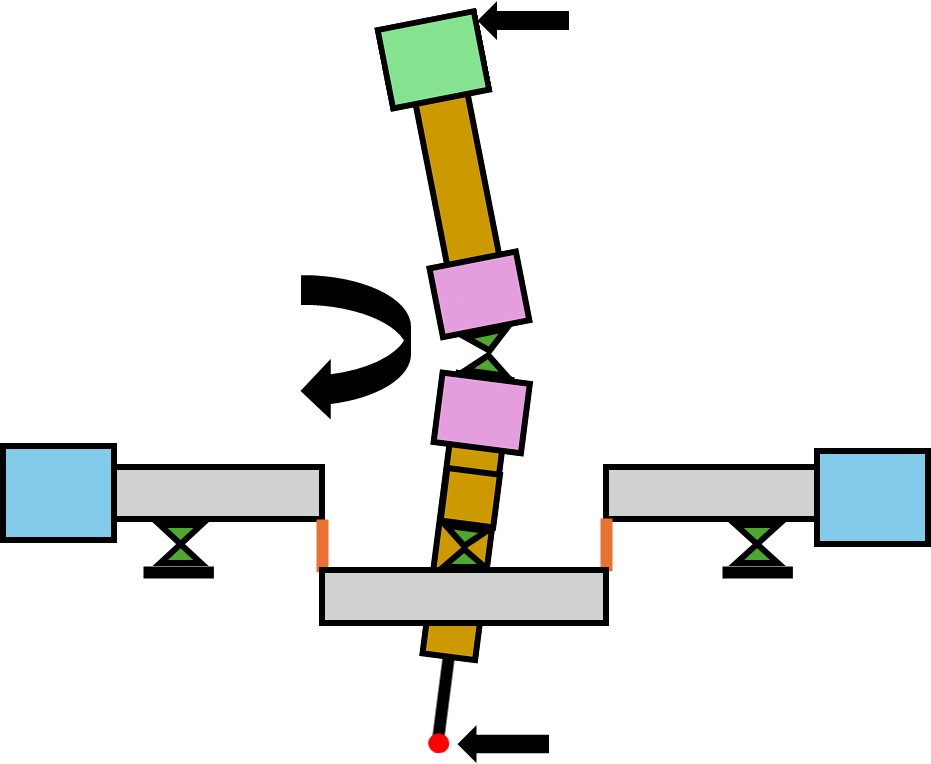
\includegraphics[width=\linewidth]{images/flyforce_xy.jpg} 
        \caption{Rotation en x ou y}  
        \label{fig:mouvement_xy}
    \end{minipage}
\end{figure}



\subsubsection{Principe de mesure des déformations du corps d’épreuve}
La mesure des déformations du corps d'épreuve se fait grâce 3 capteurs capacitifs \textbf{CSH1FL-CRm1,4} (voir \hyperref[Annexes]{Annexes}). La mesure du déplacement selon z est la plus simple car le mouvement vertical étant entièrement transmis jusqu'au sommet du mécanisme, il suffit de placer un capteur parallèlement à l'une des faces horizontales montante pour mesurer le déplacement. Selon les axes X et Y, la mesure se fait au niveau du double pivot central, légèrement au dessus pour des raisons pratiques (voir figure \ref{fig:schema_excel}). Cette particularité a été déterminante dans la conception de notre mécanisme, car cette partie du palpeur effectue un mouvement de rotation. Notre capteur étant fixe et situé sur le bâti, il fallait que le mouvement de rotation ne dépasse pas 1° d'amplitude (voir section \ref{sub:Deplacements_cible}) pour garder la surface de mesure raisonnablement parallèle au capteur et ainsi rester précis. Ce critère à été déterminant lors du dimensionnement du mécanisme complet.


\subsubsection{Mise en évidence des concepts originaux}

Notre principal atout d’originalité réside dans le design monobloc du mécanisme. En effet, une seule pièce assure l’ensemble des fonctions requises par le cahier des charges (hors contremasses et vis), comme illustré en figure \ref{fig:schema_excel}. Ce choix de conception nous a conduits à opter pour un usinage par électroérosion à fil. Ce procédé permet non seulement de réaliser une géométrie complexe en une seule étape, mais aussi d’éviter les problèmes d’assemblage liés aux hyperstatismes des tables à lames parallèles. Par ailleurs, une des particularités de notre mécanisme est qu’il repose sur de très faibles mouvements en rotation. Cela a nécessité d’assurer une rigidité relativement élevée au niveau des guidages flexibles, afin de respecter le cahier des charges. 

\vspace{2em}
\subsection{Schéma cinématique du corps d’épreuve}

\begin{wrapfigure}{r}{0.45\linewidth}  % "r" pour à droite, 0.4 pour la largeur
    \centering
    \vspace{-7em}  % ajuste la hauteur verticale si nécessaire
    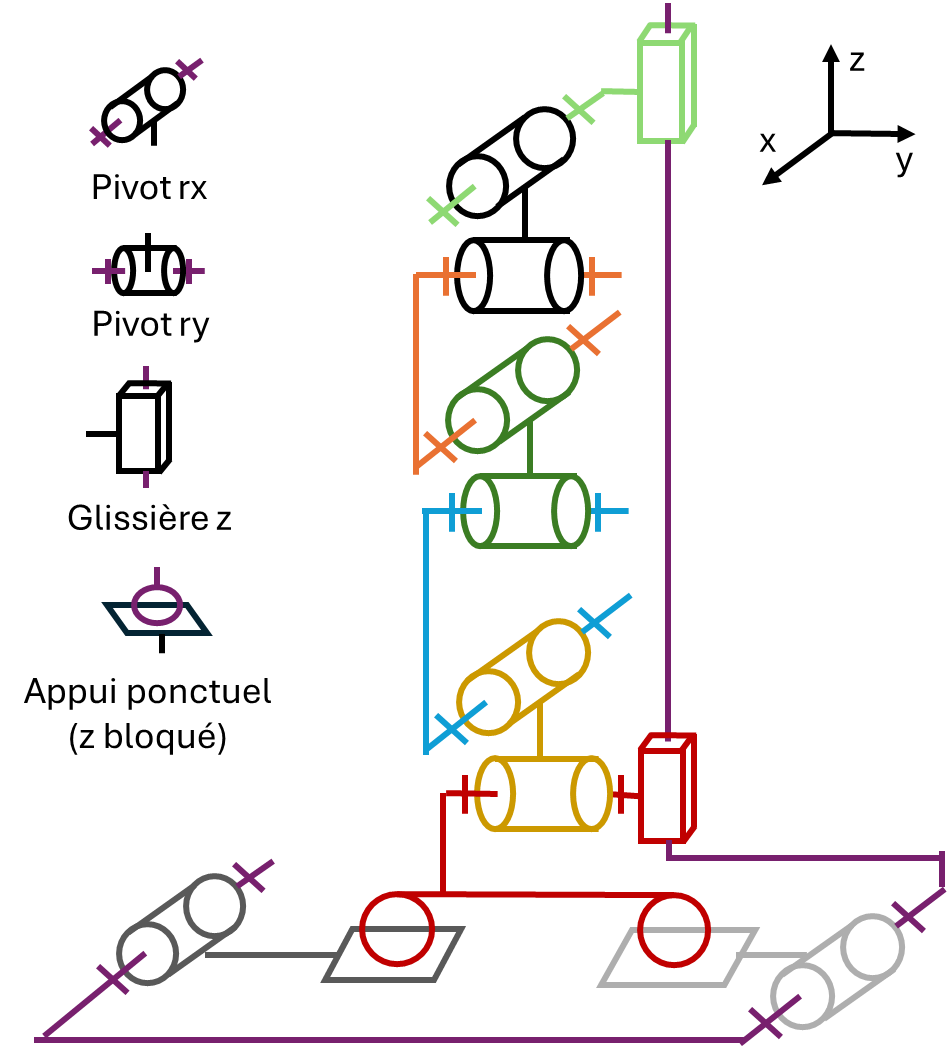
\includegraphics[width=\linewidth]{images/schéma_cinématique4.png}
    \caption{Schéma cinématique}
    \label{fig:planche}
\end{wrapfigure}

Voici notre schéma cinématique, consistant de 8 pivots, 2 glissières et 2 appuis ponctuels qui remplacent les biellettes 3D dans la cinématique idéale du rendu 1.

\vspace{5em}


\newpage
\subsection{Calcul de la mobilité selon Grübler et discussion des hyperstatismes}

\textbf{Articulations :}

\begin{itemize}
    \item pivot (×6) : 1 DOF
    \item biellette 3D (×2) : 5 DOF
    \item rotule (×1) : 3 DOF
    \item glissière (×2) : 1 DOF
\end{itemize}

\textbf{Grübler }:
 $$ k = 11, \quad n = 9, \quad b = k - n + 1 = 3 \quad  \sum d_i =  6 \cdot 1 + 2 \cdot 5 + 1 \cdot 3  + 2 \cdot 1= 21 $$



 \[M_\text{3D} = \sum d_i - 6b = 21 - 6 \cdot 3 = 3\Rightarrow DOH = DOF - M_\text{3D} = 3 - 3 = 0\]

 Nous avons donc \textbf{aucun hyperstatisme en guidages idéaux}.
\subsection{Implémentation de la cinématique du corps d’épreuve en guidages flexibles}
    Comme expliqué ci-dessus, le mécanisme utilise deux rotations et une translation.
\subsubsection*{Implémentation de la translation en Z}
\begin{figure}[H]
    \centering
    \begin{minipage}[t]{0.58\linewidth}
    \vspace{0pt}
        La translation en Z est permise par deux tables à lames parallèles fixées au bâti (entourées en figure \ref{fig:schema_excel} dans les sections E et C). Ces tables sont appelées ETAL et CTAL respectivement par simplification dans la suite du rapport.

        Lorsque le stylet fixé à la pièce en bleu clair se déplace selon z, les tables à lames transmettent le mouvement jusqu'à la masse située en haut du mécanisme.

        L'équilibrage selon Z est quant à lui permis par 2 lames et 2 pivots (figure \ref{fig:bras_levier}). La lame et le pivot permettent au bras de levier (entouré en figure \ref{fig:schema_excel} dans la section B) de pivoter et ainsi faire descendre la masse lorsque le stylet monte.
    \end{minipage}
    \hfill
    \begin{minipage}[t]{0.38\linewidth}
        \vspace{0pt}
        \centering
        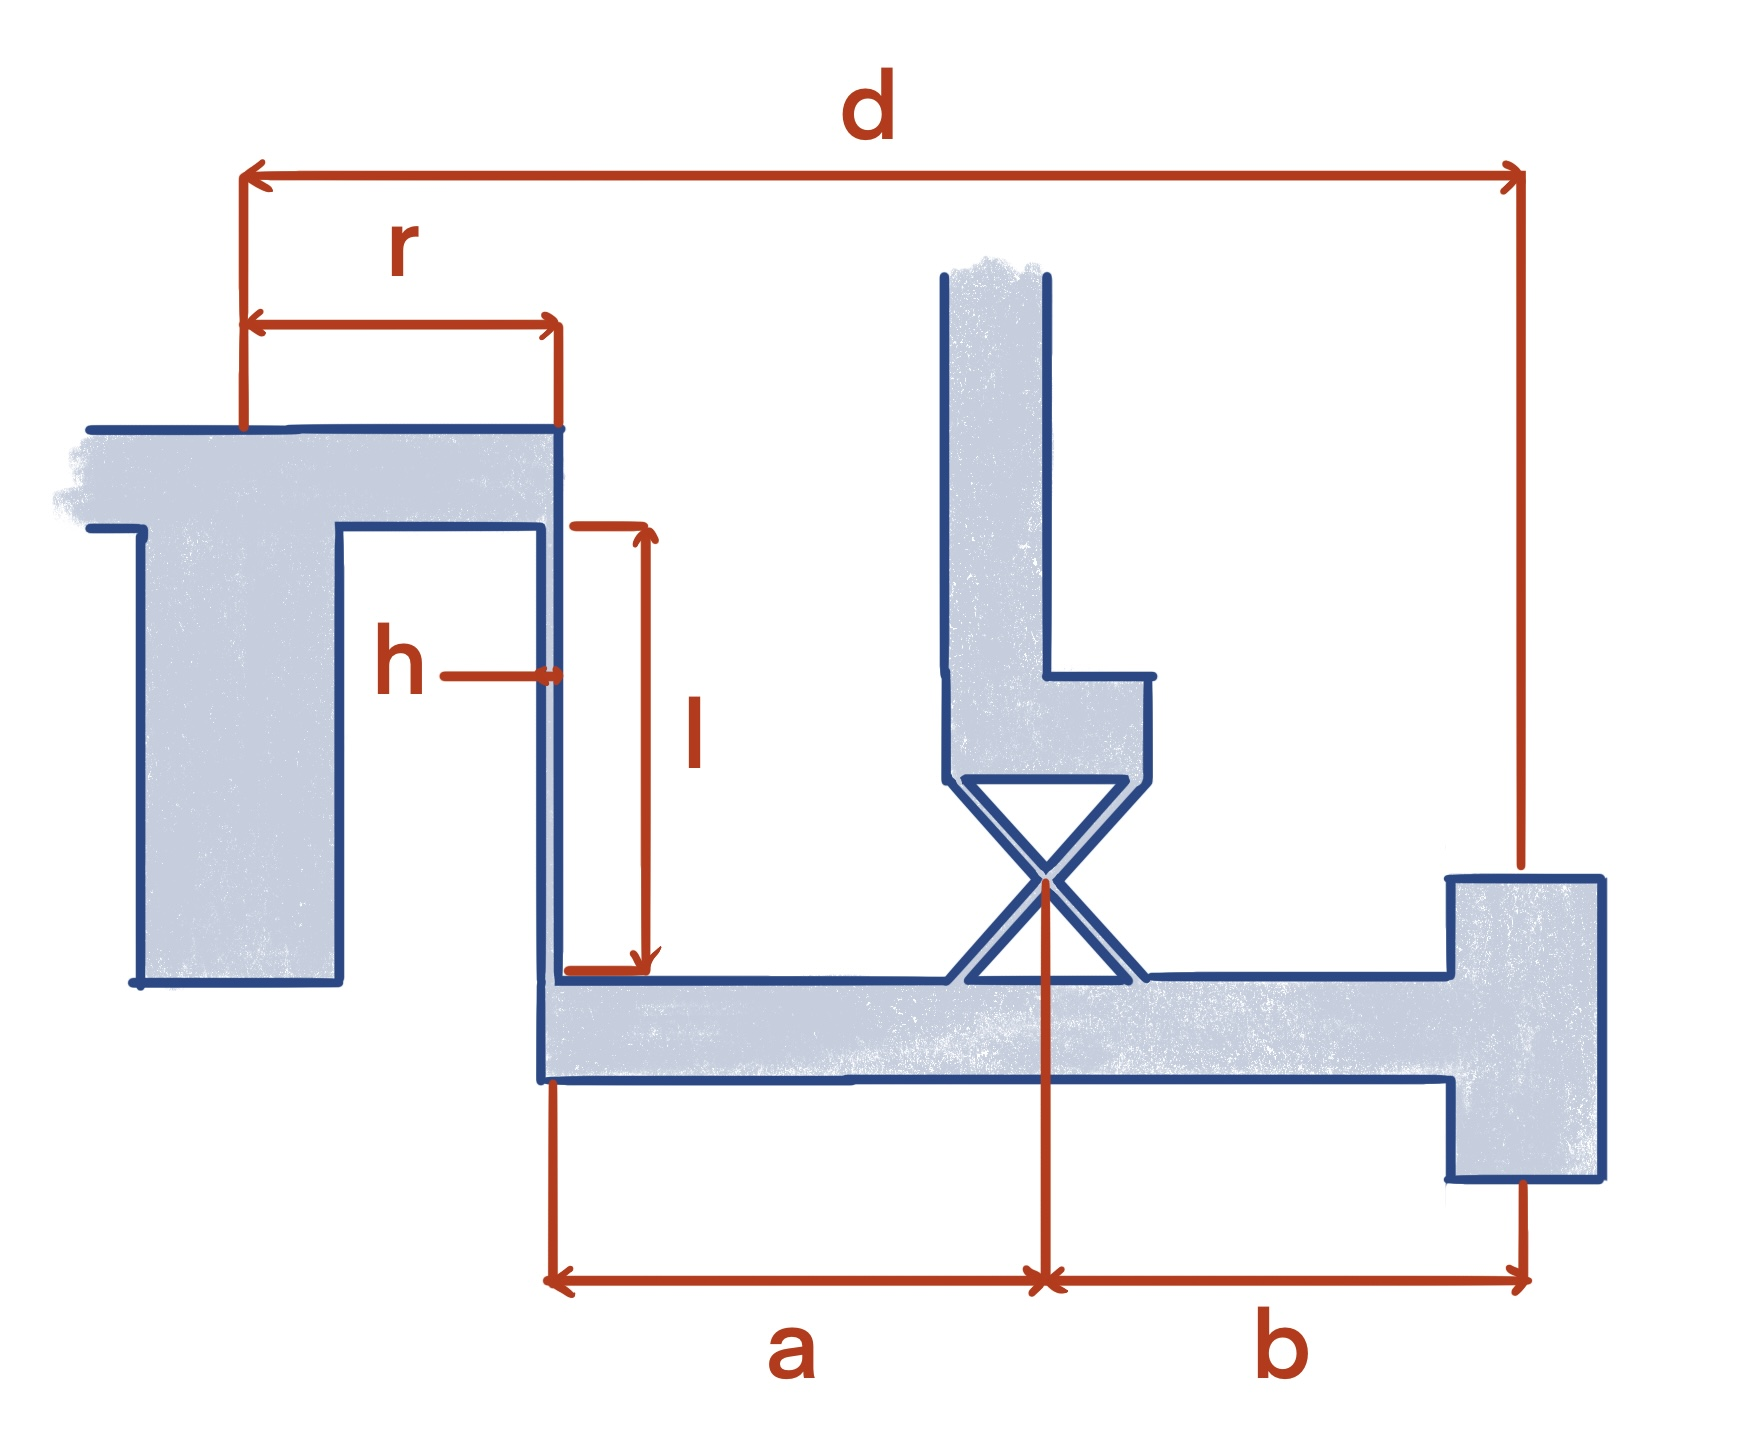
\includegraphics[width=\linewidth]{Bras_de_levier.jpeg}F
        \caption{Schéma dimensions équilibrage Z (partie B de la figure \ref{fig:schema_excel})}
        \label{fig:bras_levier}
    \end{minipage}
\end{figure}


\subsubsection*{Implémentation des rotations en X et Y}
Les rotations pour un déplacement du stylet en X et en Y fonctionnent de manière identique. \\
Les rotules sont implémentées par des doubles pivots à lames croisées non séparées (sections A, D, E, figure \ref{fig:schema_excel}). Le détail du choix des pivots est détaillé en section \ref{choix_construction}. 
Ces doubles pivots permettent au mécanisme d'effectuer des rotations autour des axes x et y. Par conséquent, la partie bleu clair du bas (l1+l2) est reliée à la partie du haut (l3+l4) par le double pivot entouré en D sur la figure \ref{fig:schema_excel}. \\ Le double pivot inférieur étant fixé au bâti, une légère translation de la partie supérieure selon z est observée (<20 $\mu $m) et est permise par ETAL.


\begin{figure}[H]
    \centering

    \begin{minipage}[b]{0.4\linewidth}
        \centering
        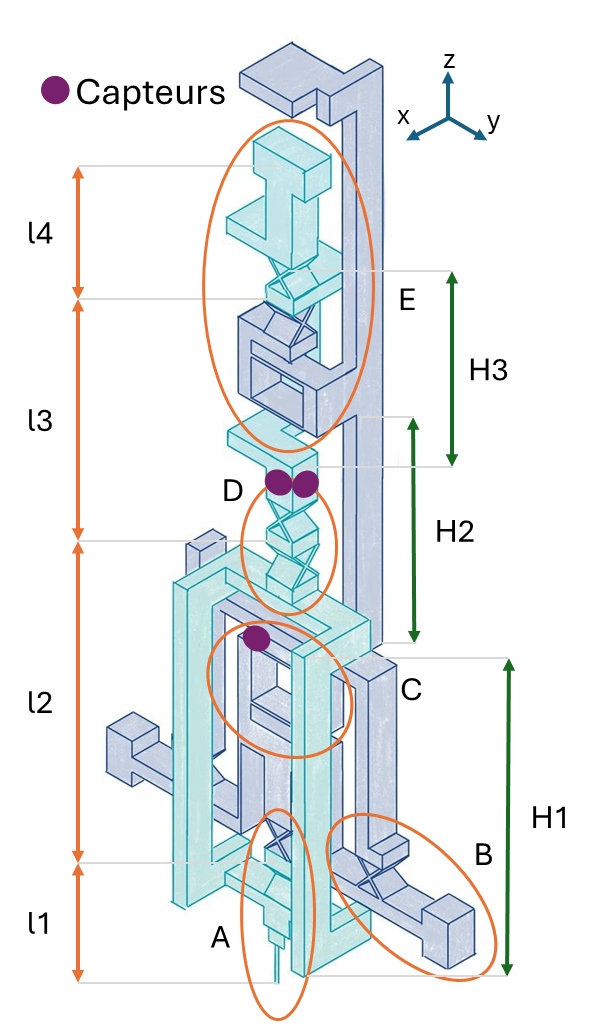
\includegraphics[height=12cm]{images/schema_dimensions.png}
        \caption{Schéma guidages flexibles }
        \label{fig:schema_excel}
    \end{minipage}
    \hfill
    \begin{minipage}[b]{0.59\linewidth} % léger ajustement à 0.59 pour compenser \hfill
        \centering
        \includegraphics[height=12cm]{images/schema_dim_lames.jpeg}
        \caption{Schéma dimensions des lames}
        \label{fig:schema_dimensions}
    \end{minipage}
\end{figure}
\vspace{3em}
\section{Dimensionnement détaillé}

\subsection{Notation et définition des grandeurs mécaniques}

Dans cette section, nous définissons et nommons l’ensemble des grandeurs utilisées. Les valeurs de ces paramètres ont été choisies en amont, puis validées a posteriori à l’aide des calculs présentés dans les sections suivantes. 


\begin{table}[H]
\centering
\renewcommand{\arraystretch}{1.2}
\begin{tabular}{|l|l|l|}
\hline
\rowcolor[gray]{0.9}
\textbf{Catégorie} & \textbf{Paramètre} & \textbf{Valeur} \\
\hline
\textbf{Déplacement en entrée} & \text{$(x, y, z)_{\text{in}}$} [mm] & \text{1} \\

\hline
\multirow{3}{*}{\textbf{Matériau}} 
& $\sigma_{\text{adm}}$ [MPa] & 2000 \\
& $E$ [GPa] & 193 \\
& $\rho$ [g/mm$^3$] & 0{,}008 \\
\hline
\multirow{4}{*}{\textbf{Encombrement}} 
& $l_1$ [mm] & 210,5 \\
& $l_2$ [mm] & 45 \\
& $l_3$ [mm] & 60 \\
& $l_4$ [mm] & 58,5 \\
\hline
\multirow{2}{*}{\textbf{Levier Z}} 
& $a$ [mm] & 9,5 \\
& $b$ [mm] & 16,75 \\
\hline
\multicolumn{3}{|c|}{\textbf{Guidages flexibles Z}} \\
\hline
\multirow{4}{*}{\textbf{Table à lame (TAL)}} 
& $b$ [mm] & 10 \\
& $e$ [mm] & 10 \\
& $h$ [µm] & 125 \\
& $L$ [mm] & 15 \\
\hline
\multirow{3}{*}{\textbf{Pivots (Z)}} 
& $b$ [mm] & 10 \\
& $h$ [µm] & 60 \\
& $L$ [mm] & 10 \\
\hline
\multirow{3}{*}{\textbf{Lames (Z)}} 
& $b$ [mm] & 10 \\
& $h$ [µm] & 60 \\
& $l$ [mm] & 15 \\
\hline
\multicolumn{3}{|c|}{\textbf{Guidages flexibles XY}} \\
\hline
\multirow{3}{*}{\textbf{Pivots (XY)}} 
& $b$ [mm] & 10 \\
& $h$ [µm] & 450 \\
& $L$ [mm] & 5 \\
\hline
\end{tabular}
\caption{Résumé des paramètres mécaniques et géométriques}
\end{table}

\subsection{Calcul de cinématique}
\label{cinématique}

\subsubsection*{Cinématique selon l'axe Z}
Lorsque l’on applique une force selon l’axe \( Z \), le palpeur se déplace verticalement vers le haut. Ce mouvement entraîne avec lui toute la partie centrale du système, qui suit une cinématique purement verticale.

Les contrepoids du système sont montés sur pivots.Ces contrepoids décrivent donc un mouvement de rotation autour de leur pivot respectif.

On a donc :

$$
\alpha_z = \arcsin\left(\frac{z_{\text{in}}}{a}\right)  = \arcsin\left(\frac{1}{9,5}\right) \approx 6^\circ \approx 0{,}1 \, \text{rad}
$$

\subsubsection*{Cinématique selon l'axe X et Y}
Le fonctionnement cinématique selon les axes X et Y est traité de manière similaire, ce qui est acceptable car la distance entre les centres des deux pivots qui forment la rotule est négligeable devant les $l_i$ nous considérons donc des rotules à la place des deux pivots dans la suite.

Lorsque l’on applique un déplacement  $x_{\text{in}}$ (ou  $y_{\text{in}}$ ) au niveau du palpeur, celui-ci décrit une rotation autour d’une rotule, notée ici rotule 1. Cette rotation entraîne une rotation opposée du contrepoids autour d’une autre rotule (rotule 3), les deux parties étant reliées mécaniquement par la rotule 2.

\begin{figure}[H]
    \centering
    
    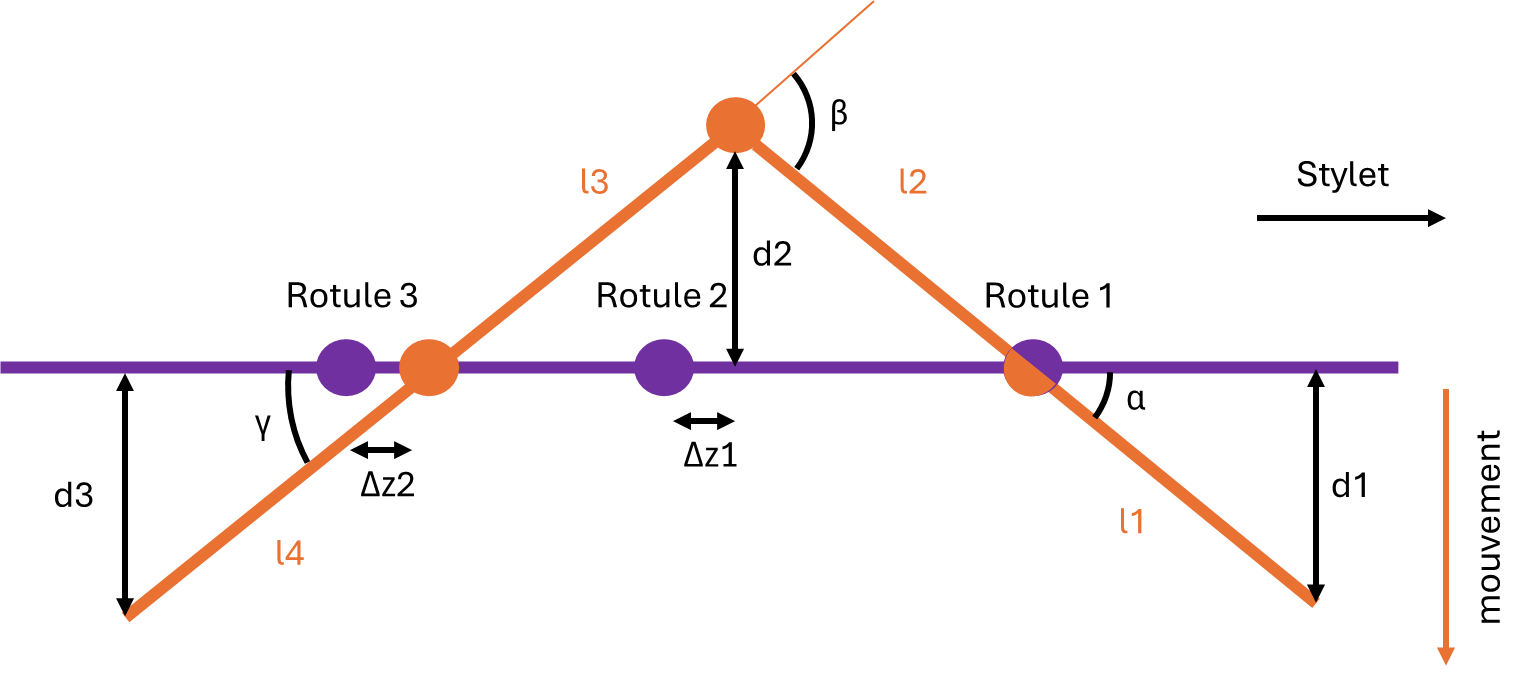
\includegraphics[width=1\linewidth]{images/trippitroppo.png}
    \caption{Cinématique des rotations}
    \label{fig:dessin cinematique}
\end{figure}


Ce système induit une série de rotations que l’on peut modéliser à travers trois angles :
\begin{itemize}
    \item  \( \alpha \) : rotation du palpeur autour de la rotule 1,
    \item  \( \beta \) : rotation de la rotule de liaison rotule 2
    \item  \( \gamma \) : rotation du contrepoids autour de la rotule 3.
\end{itemize}




Ces angles sont donnés par les relations géométriques suivantes pour un $x_{\text{in} } = 1 \, \text{mm}$   :

\[
\alpha = \arctan\left( \frac{x_{\text{in}}}{l_1} \right) \approx 0,27^\circ \approx 0{,}0048 \, \text{rad}
\]

Le déplacement \( d_2 \) de la rotule centrale (rotule 2) s’exprime comme :

\[
d_2 = \frac{l_2}{l_1} \cdot x_{\text{in}} \approx 0,24
 \text{mm}
\]

Ce qui permet d'estimer l'angle de la rotule 3 \( \gamma \) :

$$
\gamma = \arctan\left( \frac{d_2}{l_3} \right) \approx 0,21^\circ \approx 0,0037\, \text{rad}
$$

L’angle de la rotule 2 est la somme des deux autres angles:

\[
\beta = \alpha + \gamma \approx 0,48^\circ
 \approx 0,008
 \, \text{rad}
\]

Enfin, cette cinématique engendre un léger décalage vertical parasite des rotules 2 et 3, que l’on peut estimer par :

$$
\Delta z_1 = l_3 (1 - \cos(\gamma)) \approx 4,5
\times 10^{-4}\text{mm}
$$

$$
\Delta z_2 = l_2 (1 - \cos(\alpha)) + \Delta Z_1 \approx 1\times 10^{-3}\text{mm}
$$



Ces valeurs sont très faibles et seront négligées dans la suite de l'analyse.

\subsection{Contraintes dans les articulations flexibles}
\subsubsection*{Contraintes des pivots à lames croisées en rotation}

Pour ces articulations, la contrainte maximale est donnée par la formule :
\[
\sigma_\text{max} = \frac{4Eh}{l} \cdot \theta
\]

avec $\theta$ l'angle de rotation du pivot, \textit{h} l'épaisseur des lames, \textit{l} la demi-longueur des lames et \textit{E} le module de Young du matériau utilisé.

En prenant un facteur de sécurité de $3$ et $\theta = \alpha$, $\beta$ et $\gamma$ pour les doubles pivots 1, 2 et 3 respectivement, on obtient (pour un $\sigma_\text{adm} = 2000 \text{ MPa}$):

\[
\sigma_{\text{max,1}} = 3\cdot323,9 \approx 971,7
\ \text{MPa} < \sigma_{\text{adm}}
\]
\[
\sigma_{\text{max,2}} = 3\cdot579,9 \approx 1739,8
 \text{ MPa} < \sigma_{\text{adm}}
\]
\[
\sigma_{\text{max,3}} = 3\cdot256 \approx 768,1
 \text{ MPa} < \sigma_{\text{adm}}
\]
Par symétrie, ces contraintes sont identiques en X et Y.

Concernant les 2 pivots responsables de l’équilibrage du stylet en Z (entourés dans la partie B de la figure \ref{fig:schema_excel}), avec un angle $\theta = \alpha_z$,on obtient :   

$$
\sigma_{\text{max,pivots Z}} = 3\cdot488,5 \approx 1465,5\text{ MPa} < \sigma_{\text{adm}}
$$

\subsubsection*{Contraintes des tables à lames parallèles}
La contrainte maximale dans les tables à lames parallèles est donnée par : 
\[
\sigma_\text{max} = \frac{3Eh}{l} \cdot z_{in}
\]
Pour \( z_{\text{in,max}} = 1\,\text{mm} \) et un facteur de sécurité de 3, les deux tables à lames CTAL et ETAL ayant les même dimensions on obtient: 
\[
\sigma_{\text{max,TAL}} = 3\cdot 321.67 = 965
\ \text{MPa} < \sigma_{\text{adm}}
\]
Ce qui est largement en dessous de la contrainte maximale admissible du matériau, malgré le grand facteur de sécurité.

\subsection{Calculs de rigidité des articulations flexibles}\label{rigidite}
\subsubsection*{Rigidité linéaire et angulaire de chaque articulation de l'axe Z}
Le mouvement en Z est permis par trois types de guidages flexibles : 
\textbf{Table à lame (2x), Pivot à lames croisées (2x), Lame (2x).}


Nous calculons ici la rigidité de ces articulations.

\paragraph{Table à lames} :

\textbf{Formule de rigidité} : $ K_0 = \frac{24EI}{\ell^3},\ \text{où}\ I = \frac{b h^3}{12} $


$\text{Avec: } E = 192\,\text{GPa},\quad b = 10\,\text{mm},\quad h = 125\,\mu\text{m},\quad \ell = 15\,\text{mm} $


\textbf{Résultat}: $$K_0 \approx 2233,8\text{ N}/\text{m}$$

\vspace{0.25cm}

\paragraph{Pivot à lames croisées}:

\textbf{Formule de rigidité angulaire}:
$K_\theta = \frac{8EI}{\ell}, \quad \text{où} \quad I = \frac{b h^3}{12}$



$\text{Avec: } E = 192\,\text{GPa},\quad b = 10\,\text{mm},\quad h = 60\,\mu\text{m},\quad \ell = 10\,\text{mm} $


\textbf{Résultat} : $$K_\theta \approx 0,028\text{ N}\text{m}/\text{rad}$$
 
 \paragraph{Lame RCC (approximation pivot RCC)}:
 
Pour le cas des lames, nous faisons l'approximation selon laquelle la lame tourne autour d'elle-même autour d’un axe $x$. De ce fait, la lame se comporte comme une lame d’un pivot RCC, ce qui engendre une rigidité angulaire deux fois plus faible et $\rho = 0$.

\textbf{Formule de rigidité angulaire pivot RCC} :
\[
K_\theta = \frac{8EI (\ell^2 + 3\rho\ell + 3\rho^2)}{\ell^3}
\quad \text{avec} \quad I = \frac{b h^3}{12}
\]

Dans le cas particulier où $\rho = 0$ et $K_{\theta\ lame} = \frac{K_\theta}{2} $ , cette formule se simplifie :
\[
K_{\theta\ lame} = \frac{8EI}{2\ell}
\]


$\text{Avec: } E = 192\,\text{GPa},\quad b = 10\,\text{mm},\quad h = 60\,\mu\text{m},\quad \ell = 15\,\text{mm} $


\textbf{Résultat} :
$$
K_{\theta\ lame} \approx 0,044\cdot\text{N}\text{m}/\text{rad}
$$
\subsubsection*{Calcul de la rigidité équivalente selon l'axe Z}
Selon l’axe $Z$, le système comporte 2 pivots, 2 tables à lames et 2 lames RCC. La rigidité équivalente $k_{\text{eq z}}$ est déterminée par l’addition des énergies potentielles.


$$
\frac{1}{2} k_{\text{eq z}} z_{\text{in}}^2 = \frac{1}{2} \sum k_i z_i^2 + \frac{1}{2} \sum K_{\theta j} \alpha_j^2 = \sum E_{\text{pot}}
$$
Avec (voir cinématique) :
$ z_{\text{in}} = z_{\text{TAL}} =1\, \text{mm},\quad \alpha_{\text{z,lame}} \approx \alpha_{\text{z,pivot}}\approx \alpha_{\text{z}} \approx 0.1\, \text{rad }$


On en déduit :
$$
k_{\text{eq}_Z} = \frac{2 \sum E_{\text{pot}}}{z_{\text{in}}^2} \approx 5,28
 \, \text{N/mm}
$$
 Cela respecte le cahier des charges, qui impose une rigidité de \(5\,\text{N/mm} \pm 10\%\)

\subsubsection*{Rigidité linéaire et angulaire de chaque articulation de l'axe X et Y}
L'axe X et Y sont des rotations, qui sont guidées par \textbf{trois pivots à lames croisées} et \textbf{une table à lames}. Contrairement à l'axe Z, le déplacement de la table à lames (ETAL)est très faible ($\ll 1\,\text{mm}$) et ne contribue que très peu à la rigidité globale (ici négligée). De plus, les angles de déplacement sont très faibles. Pour respecter le cahier des charges, nous avons donc choisi une épaisseur de lame pour les pivots relativement élevée pour augmenter la rigidité.


\paragraph{Pivot à lames croisées}:

\textbf{Formule de rigidité angulaire} :\(K_\theta = \frac{8EI}{L}, \quad \text{avec} \quad I = \frac{b h^3}{12}\)


$ \text{Avec: } E = 192 \, \text{ GPa } , b = 10 \, \text{mm}, h = 450 \, \mu\text{m}, L = 5 \, \text{mm} $


\textbf{Résultat} : $$K_\theta \approx 23,5
 \cdot\text{N}\text{m}/\text{rad}$$




\subsubsection*{Calcul de la rigidité équivalente selon l'axe X et Y}

Comme vu avant, nous pouvons calculer le $k_{\text{eq xy}}$. 

Avec (voir cinématique) :
$ x_{\text{in}} = 1\, \text{mm},\quad \alpha \approx 0,0047\text{ rad, }
\beta \approx 0,008
\text{ rad, } \gamma \approx 0,0037\, \text{rad},$


On en déduit :
$$
k_{\text{eq xy}} = \frac{2 \sum E_{\text{pot}}}{x_{\text{in}}^2} \approx 4,93\text{ N/mm}
$$

\subsection{Calcul des masses pour l'équilibrage}\label{sub:labelito}
Notre mécanisme doit être équilibré en force et en moment. Ainsi, sa quantité de mouvement et son moment cinétique doivent rester nuls dans tout son espace de travail.

\vspace{1em}

\noindent
\begin{minipage}[t]{0.50\textwidth}

\subsubsection*{Masses du mécanisme}
Le tableau \ref{tab:masse} présente un aperçu de la masse des différentes pièces de notre mécanisme. Ainsi, nous savions avant de dimensionner les contrepoids que leur masse ne devait pas dépasser les 300g environ.

\end{minipage}
\hfill
\begin{minipage}[t]{0.45\textwidth}
\vspace*{-2.5 em} % Ajuste cette valeur pour aligner parfaitement avec le texte
\begin{table}[H]
\centering
\begin{tabular}{|l|c|}
\hline
\textbf{Élément} & \textbf{Masse (g)} \\
\hline
Châssis & 163 \\
Supports capteurs & 44 \\
Capteurs (câbles inclus) & 90 \\
Corps principal & 382 \\
Vis & 18 \\
\hline
\textbf{Total} & \textbf{697} \\
\hline
\end{tabular}
\caption{Masses du mécanisme}
\label{tab:masse}
\end{table}
\end{minipage}

\newpage

\subsubsection*{Tentative de dimensionnement avec le stylet 100g}
\noindent
\begin{minipage}[t]{0.65\textwidth}
Nous avons d'abord essayé de dimensionner les masses du contrepoids en utilisant le stylet 100g. Cependant, avec ce stylet, il était impossible de poser le centre de masse sur le pivot du bas. Nous avons donc essayé d'équilibrer les axes X et Y simultanément en force et en moment. Après avoir tenté de résoudre ce problème par tâtonnement, le nombre de paramètres libres et la limitation du poids maximal nous ont poussés à procéder numériquement. La figure \ref{fig:dessin_masse1} montre le schéma du problème. La pièce A, d'inertie $I_A$ et de masse $m_A$, représente le stylet et son support. La pièce B, d'inertie $I_B$ et de masse $m_B$, représente le support des masses. Les dimensions $L$, $r_2$, $r_3$ et $r_4$ de ces pièces sont également fixées. Les variables libres sont les masses des deux contrepoids, $m_1$ et $m_2$, ainsi que la position de la rotule du haut par rapport au centre du contrepoids, $r_1$. On cherche à minimiser la masse totale $M = m_1 + m_2$ des masses d'équilibrage sous la contrainte que la quantité de mouvement et le moment angulaire du mécanisme soient nuls. 
\begin{gather*}
\sum_i^N m_i \vec{v_i} = 0 \\
\sum_i^N I_i \vec{\omega_i} = 0 
\end{gather*}

Nous avons pu ramener ces contraintes à un problème de minimisation d'un problème linéaire. Les deux équations encodent les deux contraintes d'équilibrage et les deux inconnues sont les masses $m_1$ et $m_2$:

\vspace{1em}

$$
A =
\begin{bmatrix}
\frac{\frac{L}{2} - r_1}{r_1} & -\frac{\frac{L}{2} + r_1}{r_1} \\
\left( \frac{L}{2} - r_1 \right)^2 & \left( \frac{L}{2} + r_1 \right)^2
\end{bmatrix}
$$
$$
\vec{x} = 
\begin{bmatrix}
m_1 \\
m_2
\end{bmatrix}
\quad
\vec{b}=
\begin{bmatrix}
m_B - \dfrac{(r_1 + r_2)r_4}{r_1 r_3} m_A \\
\dfrac{r_1 + r_2}{r_3}(I_A + m_A r_4^2) - (I_B + m_B r_1^2)
\end{bmatrix}
$$

\vspace{1em}

Nous avons ensuite minimisé la fonction $M = m_1 + m_2$ en fonction de $r_1$. Le programme en section \ref{prog} résout numériquement ce problème avec les dimensions de notre mécanisme. Le résultat de l'optimisation est présenté à la figure \ref{massimo}. Nous obtenons des contrepoids de masses minimale $M = 804\text{g}$. 
\end{minipage}
\hfill
\begin{minipage}[t]{0.3\textwidth}
    \begin{figure}[H]
        \centering
        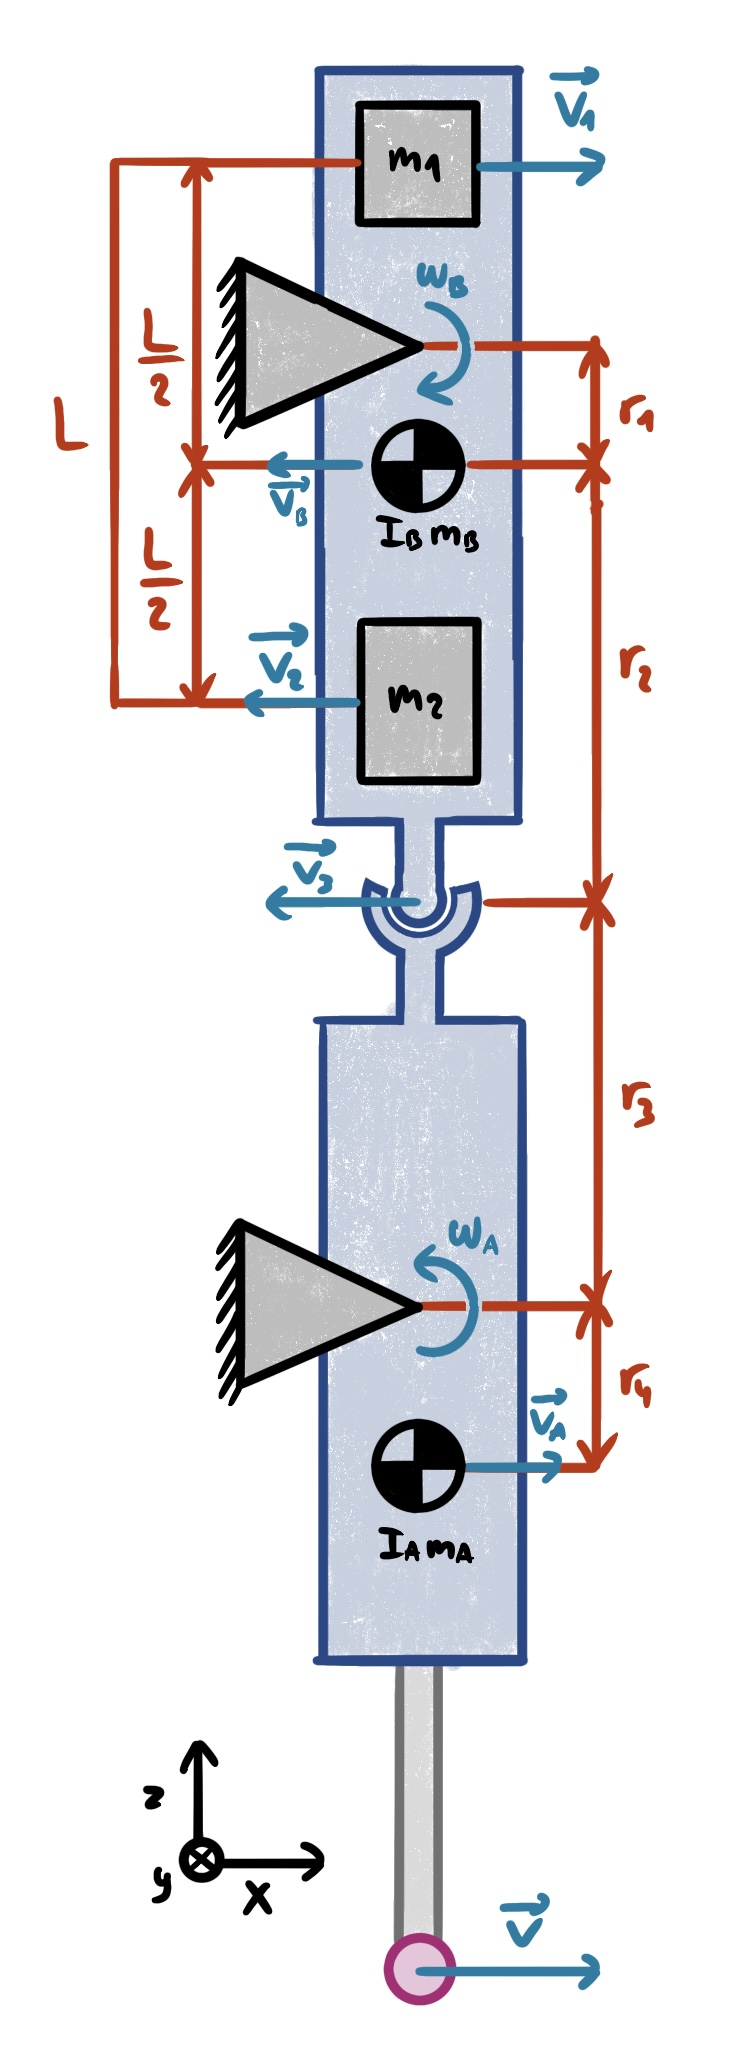
\includegraphics[width=\linewidth]{IMG_0691.jpeg}
        \caption{\raggedright Schéma du dimensionnement avec stylet 100g}
        \label{fig:dessin_masse1}
    \end{figure}
    \vfill
    \begin{figure}[H]
        \centering
        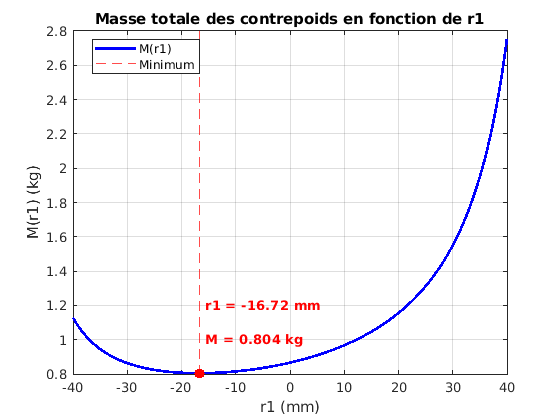
\includegraphics[width=\linewidth]{images/masses.png}
        \caption{Masse totale des contrepoids en fonction de r1}
        \label{massimo}
    \end{figure}
\end{minipage}

\newpage

Il ressort de cette analyse que les masses d'équilibrage pour les axes X et Y seraient trop lourdes avec le stylet de 100g. De plus, comme notre mécanisme fonctionne en série, les masses pour l'équilibrage en Z devraient être d'autant plus lourdes pour compenser celles-ci, ce qui crée un effet boule de neige considérable. D'autre part, après avoir calculé la densité du stylet et après une comparaison avec d'autre modèles de stylet de cette dimension, une masse de 10g nous semble plus réaliste. Notre mécanisme est donc conçu pour un stylet de 10g.



\subsubsection*{Axes X et Y}
Nous traitons l'axe X et Y simultanément en considérant les pivots doubles comme des rotules. La figure \ref{equ_xy} montre le schéma cinématique simplifié que nous avons utilisé afin d'équilibrer cette section du mécanisme. Avec le nouveau stylet, nous avons pu positionner le centre de masse des deux pièces sur leurs centres de rotation. Ainsi, la quantité de mouvement de chaque pièce est nulle et il nous a suffit de faire correspondre les moments angulaires pour déterminer l'inertie nécessaire du contrepoids:
$$
I_1\omega_1 = I_2\omega_2 \quad \Leftrightarrow \quad I_1 = \frac{r_1}{r_2}I_2
$$
Ensuite, nous avons pu procéder par tâtonnement pour que la pièce du haut possède cette inertie et que son centre de masse se situe sur son pivot. Les erreurs induites par les distances entre les centres de masse et de rotation et les différences entre les moments cinétiques réels seront traitées dans la section concernant les erreurs de mesures (voir section \ref{sub:bonecaambalabu}).
\begin{figure}[H]
    \centering
    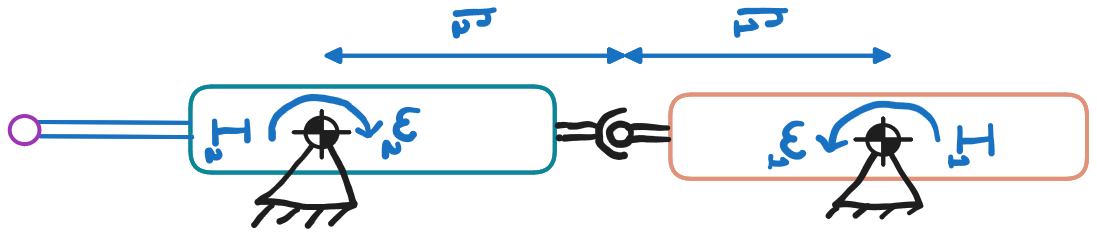
\includegraphics[width=0.5\linewidth]{images/equilibrageXY_schema.png}
    \caption{Schéma des axes X et Y}
    \label{equ_xy}
\end{figure}


\subsubsection*{Axe Z}
Pour cette axe, nous utilisons le modèle dessiné à la figure \ref{equ_z}. Par symétrie, les deux contrepoids ont la même inertie et des vitesses angulaires opposées. Ainsi, leurs moments angulaires s'annulent lors du mouvement vertical du stylet. Concernant la quantité de mouvement, nous avons supposé que l'axe de rotation des deux poutres latérales passe par le centroïde de ces dernières. Nous avons donc ignoré leur quantité de mouvement dans nos calculs.
\begin{figure}[H]
    \centering
    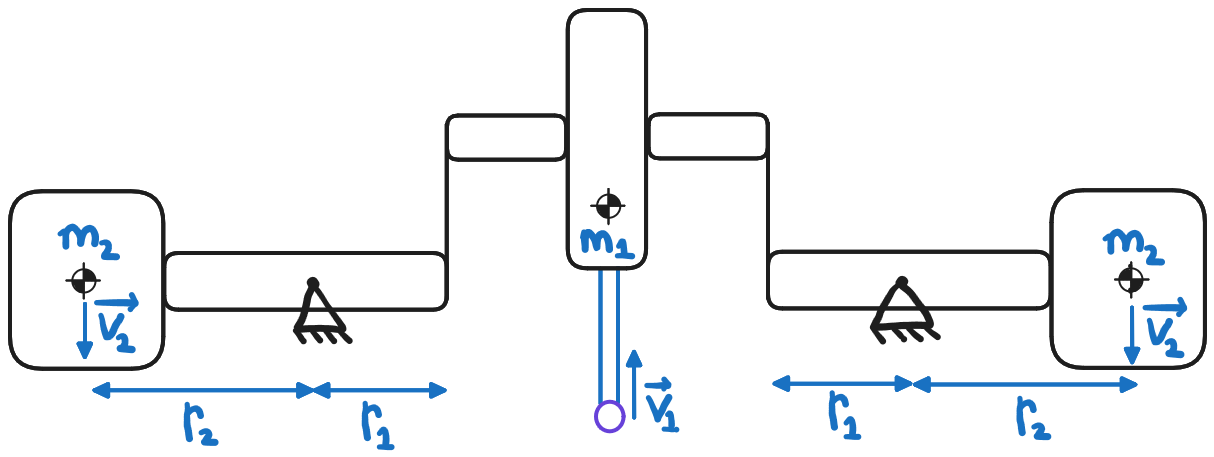
\includegraphics[width=0.5\linewidth]{images/equilibrageZ_schema.png}
    \caption{Schéma de l'axe Z}
    \label{equ_z}
\end{figure}
Pour dimensionner les contrepoids, nous avons d'abord choisi leur matériau et donc leur densité. Ensuite, nous avons fait un premier dessin sur le plan XY de l'empreinte des masses. Cela nous a permis de déterminer la position du centre de masse et sa distance avec le centre de rotation du pivot. Puis, nous avons déterminé la masse nécessaire pour contrebalancer le reste du mécanisme en annulant la quantité de mouvement totale. Finalement, nous avons adapté la hauteur des contrepoids pour que leur poids correspond.
$$
m_1v_1 = 2m_2v_2 \quad \Leftrightarrow \quad m_2 = \frac{r_1}{2r_2}m_1
$$
Les différences entre le modèle théorique et la réalité sont discutées dans la section erreur de mesure (voir section \ref{sub:erreur_mesure}).

\begin{minipage}[t]{0.50\textwidth}
\subsubsection*{Masse  totale}
Le tableau \ref{tab:masse_tot} présente la masse de nos quatre masses d'équilibrage. Au total, la masse de notre mécanisme est de $697 + 280 = 977\text{g}$.
\end{minipage}
\hfill
\begin{minipage}[t]{0.45\textwidth}
\vspace*{-2.5em}
\begin{table}[H]
\centering
\begin{tabular}{|l|c|}
\hline
\textbf{Élément} & \textbf{Masse (g)} \\
\hline
Masse haute & 47 \\
Masses milieu & 27 \\
Masse droite & 103 \\
Masse gauche & 103 \\
\hline
\textbf{Total} & \textbf{280} \\
\hline
\end{tabular}
\caption{Masse des contrepoids}
\label{tab:masse_tot}
\end{table}
\end{minipage}

\subsection{Déplacements des cibles des trois capteurs capacitifs}\label{sub:Deplacements_cible}
Le premier capteur, chargé de mesurer les déplacements selon l’axe z, a sa cible positionnée juste après la table à lame parallèle inférieure. Le mouvement de cette cible s’effectue principalement selon l’axe z, avec une légère composante selon l’axe x. Toutefois, comme vu précédemment, ce déplacement selon x est négligeable.

Les deux autres capteurs, qui mesurent respectivement les déplacements selon les axes x et y, sont placés au centre du mécanisme. Leurs cibles suivent un mouvement similaire, combinant des déplacements selon les axes x et z, accompagnés d’une légère rotation. D’après la fiche technique du capteur, l’angle maximal admissible est de 1°. Nous avons donc veillé à ce que la rotation de la cible reste en dessous de cette limite. Comme mentionné précédemment, l’angle $\gamma$ mesuré sur la pièce cible atteint au maximum 0.21°, ce qui respecte largement la contrainte imposée.

Enfin, étant donné que le mouvement de la cible est globalement parallèle au plan de mesure des capteurs, nous avons simplement agrandi la surface cible afin de permettre la détection sur toute la course du mécanisme, de butée à butée.


\subsection{Étude de la robustesse et protection contre les surcharges}

Des butées rigides sont intégrées au niveau du mécanisme afin de limiter la course maximale des capteurs. Elles sont positionnées légèrement au-delà de la plage utile de mesure (\(\pm 1\)~mm), de manière à ne pas interférer avec le fonctionnement normal. Leur rôle est d'empêcher tout déplacement lorsque la force appliquée dépasse 5,5~N. Le contact s'effectue entre deux parties rigides du mécanisme, conçues pour supporter sans dommage des surcharges allant au-delà de 15~N.

\textbf{Dimensionnement pour l'axe z: }
Pour avoir une butée après l'application de 5,5N, nous calculons le déplacement maximal:
$$\Delta \text{butée}_z = \frac{F}{k_{\text{eq}_Z}}= \frac{5,5}{5,28} \approx 1,04\text{ mm}$$
\textbf{Dimensionnement pour l'axe xy: } Pour une force d'entrée de 5,5 N, nous avons un $\Delta x_\text{max} \approx 1,12$ mm et par conséquent $\alpha \approx 0,3^\circ $. De plus, nous avons la distance entre le pivot et la butée qui est donnée par $l' = 47,5$ mm. Ceci nous permet de calculer les butées:
$$\Delta \text{butée}_x = \sin(\alpha)l' \approx 0,25\text{ mm}$$

\subsection{Résolution de mesure de force}
\label{resolution_force}

\subsubsection*{Résolution de force pour l'axe Z}

Pour l'axe Z, le capteur se déplace de la même manière que le palpeur. Nous avons choisi le capteur capacitif \textbf{CSH1FL-CRm1,4} (voir \hyperref[Annexes]{Annexes}), qui offre une résolution de \(20\, \text{nm}\).

La relation entre la force appliquée \(F_{\text{in}}\) et le déplacement vertical \(\delta_z\) est donnée par la rigidité équivalente de l’axe Z :
\[
\Delta z_{in} = \frac{F_{\text{in}}}{k_{\text{eq},z}} \Rightarrow F_{\text{rés}} = \Delta z_{in} \cdot k_{\text{eq},z}
\]

On peut donc en déduire la résolution de mesure de force :
\[
\Delta z_{in} = \Delta_{\text{capteur}} = 20\, \text{nm}  \Rightarrow F_{\text{rés}} = 20 \times 10^{-9} \cdot 5,28 \times 10^{3} \approx 0,11 \text{mN}
\]


\subsubsection*{Résolution de force pour les axes X et Y}

Les capteurs capacitif des axes X et Y sont se trouvent juste au dessus de la rotule 2. Ils subissent donc une rotation de $0,21^\circ$ on peut donc l'approximer comme une translation.

Le capteur utilisé est le \textbf{CSH1FL-CRm1,4} (voir \hyperref[Annexes]{Annexes}), avec une résolution de $20\, \text{nm}$.

\begin{figure}[H]
    \noindent
    \begin{minipage}{0.5\linewidth}
        Le déplacement en entrée $\Delta x_{\text{in}}$ est relié au déplacement mesuré $\Delta_{\text{capteur}}$ par la relation :
        $$
        \Delta x_{\text{in}} = \frac{l_1}{l_2} \cdot \Delta_{\text{capteur}}
        $$
        On peut donc en déduire la résolution de mesure de force :
        \begin{align*}
            \Rightarrow\ F_{\text{rés}} &= \Delta x_{\text{in}} \cdot k_{\text{eq},xy} = \left( \frac{l_1}{l_2} \cdot \Delta_{\text{capteur}} \right) \cdot k_{\text{eq},xy} \\
            &= \frac{210,5}{45} \cdot 20 \times 10^{-9} \cdot 4,92 \times 10^{3} \approx 0{,}41\, \text{mN}
        \end{align*}
    \end{minipage}
    \hfill 
    \begin{minipage}{0.5\linewidth}
    \centering
    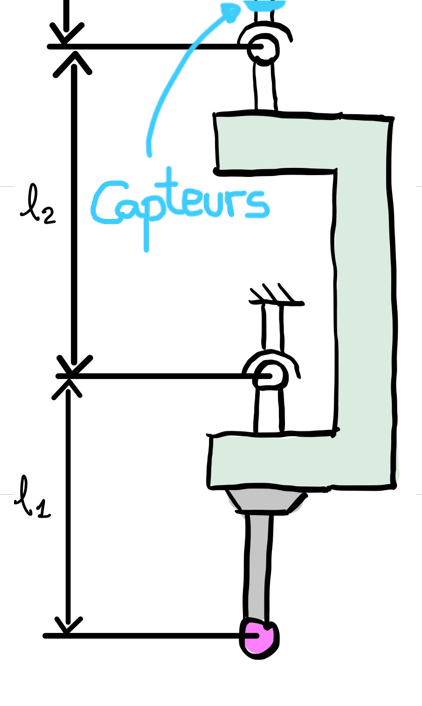
\includegraphics[width=0.7\linewidth]{images/mouvement_capteur.png}
    \caption{Rotule 1 déplacement du capteur}
    \label{fig:rotule_1}
    \end{minipage}
\end{figure}

\subsection{Gamme dynamique de la mesure de force}
\subsubsection*{Gamme dynamique de mesure de force sur l’axe Z}

On définit la gamme dynamique de mesure de force comme le rapport entre la force maximale mesurable et la plus petite variation de force détectable :

\[
\text{GD}_z = 20 \log_{10} \left( \frac{F_{\text{max}, z}}{\delta F_Z} \right)
\]

Calcul de $F_{\text{max}, z}$
$$
{F_{\text{max}, z}} = {\text{résolution}} \cdot k_{\text{eq},z} = 5,28 \text{ N}
$$


De la section \hyperref[Résolution]{Résolution de mesure de force} on a: ${\delta F_Z} = 0,11 \text{mN}$

$$
\Rightarrow \text{GD}_z = 20 \log_{10} \left( \frac{5,28}{1,1 \times 10^{-4}} \right) = 20 \log_{10}(48000) \approx 93,6 \, \text{dB}
$$
\subsubsection*{Gamme dynamique de mesure de force sur les axes X et Y}
Calcul de $F_{\text{max}, xy}$
$$
{F_{\text{max}, xy}} = \left( \frac{l_1}{l_2} \cdot {\text{résolution}} \right)\cdot k_{\text{eq},xy} = \frac{210,5}{45} \cdot 1  \cdot 4,92 = 23
\text{ N}
$$
Mais cette valeur est limitée par les butées $\Rightarrow {F_{\text{max}, xy}} = 5,5  \text{ N} $

De la section  \hyperref[Résolution]{Résolution de mesure de force} on a:
$
{\delta F_\text{xy}} = 0,41 \text{mN}
$

$$
\Rightarrow \text{GD}_\text{xy} = 20 \log_{10} \left( \frac{5,5}{4,1 \times 10^{-4}} \right) = 20 \log_{10}(13 415) \approx 82,5 \, \text{dB}
$$
\subsection{Résolution de mesure de déplacement}

\subsubsection*{Résolution de mesure pour un déplacement selon l’axe Z}

Sur l’axe Z, le capteur se déplace directement sans effet de levier ni multiplication du mouvement. Ainsi, la résolution de mesure est simplement celle du capteur lui-même, soit :

\[
\Delta z = \Delta_{\text{capteur}} = 20 \, \text{nm}
\]

\subsubsection*{Résolution de mesure pour un déplacement selon les axes X et Y}

Comme vu dans la section \ref{resolution_force}:

\[
\Delta x_{\text{in}} = \frac{l_1}{l_2} \cdot \Delta_{\text{capteur}}
\]

Avec : $  l_2 = 52 \, \text{mm}\quad l_1 = 210,5 \, \text{mm}\quad \Delta_{\text{capteur}} = 20 \, \text{nm} $

On obtient donc la résolution sur les axes X et Y :

\[
\Delta {x,y} = \frac{210.5}{45} \cdot 20 \, \text{nm} \approx 93,5 \, \text{nm}
\]

\subsection{Masse réduite de l’ensemble du mécanisme}
\subsubsection*{Masse réduite selon l'axe Z}



\[
\omega_{pivot} = \frac{v_{\text{in}}}{a} = \frac{v_{M\text{z}}}{b}
\Rightarrow v_{M\text{z}} = \frac{b}{a} v_{\text{in}}
\]

Énergie cinétique totale :
\[
\frac{1}{2} M_{\text{eq}z} v_{\text{in}}^2 = 
\frac{1}{2} (M_{\text{stylet}} + M_{milieu} + M_{haut} + M_{visses}+ M_{\text{structure}z}) v_{\text{in}}^2 
+ 2 \cdot \frac{1}{2} M_z \left( \frac{b}{a} v_{\text{in}} \right)^2
\]

D’où la masse équivalente :
\[
M_{\text{eq}z} = M_{\text{stylet}} + M_{milieu} + M_{haut}+ M_{\text{structure}z} + M_{visses} + 2 M_z \left( \frac{b}{a} \right)^2 = 1696.8  [\text{g}]
\]

\subsubsection*{Moment d'inertie réduite selon les axes X et Y}
Calcul d'inertie équivalent en pour les rotations autour des axes x et y sont similaires du a la symértie des pièces.

\begin{equation}
\frac{1}{2} I_{\text{eq}} \omega_1^2 = \frac{1}{2} I_{\text{eq,1}} \omega_1^2 + \frac{1}{2} I_{\text{eq,2}} \omega_2^2 \text {  Avec : } \omega_1l_2 = \omega_2l_3
\end{equation}

Expression de $I_{\text{eq}}$ (avec $D_1^2$  la distance entre le centre de masse du stylet et la rotule 1 et $l_3'$  la distance entre la masse milieu et la rotule 3) :

\begin{equation}
I_{\text{eq}} = I_{\text{eq,1}} + \left( \frac{l_2}{l_3} \right)^2 I_{\text{eq,2}} 
\end{equation}

$\text{Avec  } I_{\text{eq,1}} = M_{\text{stylet}} \cdot D_1^2 + I_1\text { et } I_{\text{eq,2}} = M_{\text{haut}} \cdot l_4^2 + M_{milieu} \cdot l_3'^2 + I_2$






Application numérique :

\begin{equation}
I_{\text{eq,1}} = 10 \cdot 117.5^2 + 71 \approx 209.5 ~\text{kg} \cdot \text{mm}^2
\end{equation}

\begin{equation}
I_{\text{eq,2}} = 165 \cdot 58.5^2 + 2 \cdot 0.012 \cdot 51.5^2 + 90 \approx 718.33~\text{kg} \cdot \text{mm}^2
\end{equation}

\bigskip

Calcul de $I_{\text{eq}}$ :

\begin{equation}
I_{\text{eq}} = I_{\text{eq,1}} + \left( \frac{l_2}{l_3} \right)^2 \cdot I_{\text{eq,2}} = 209.5 + 0.75^2 \cdot 718.33 = 613.56~\text{kg} \cdot \text{mm}^2
\end{equation}

On peut approximer le stylet par un cylindre tournant autour d'un de ses bouts. Dont l'équation est la suivante:$ I_{\text{eq}} = \frac{M_{\text{eq}}\cdot l_1^2}{3}$

\begin{equation}
M_{\text{eq}} = \frac{3 \cdot I_{\text{eq}}}{l_1^2} = \frac{3 \cdot613.56}{ 210.5^2} \approx 0.04154\ \text{kg} = 41.54\ \text{g}
\end{equation}


\subsection{Résistance à l’usure et analyse de la durabilité}

Pour calculer la résistance à la fatigue d'un matériau, nous utilisons la loi de Miner.

\[
\sum\frac{n_i}{N_i} = C
\]

Où $n_i$ est le nombre de cycles accumulé à un stress $S_i$ et $N_i$ est le nombre moyen de cycles pour casser au stress $S_i$. C est donc la fraction de vie consumée.

Nous avons opté pour l'acier Maraging W720 pour notre mécanisme. Ce matériau a une limite d'endurance pour 10 millions de cycles en flexion de :
\[
\sigma_d = 735 [MPa]
\]
De plus nous voulons que notre mécanisme dure plus de 10 ans avec une cadence de palpage de 2 Hertz en l'utilisant 4 heures par jour. Nous aurons donc un nombre de cycle :
\[
n_i = \frac{t}{f} = \frac{10\cdot365\cdot4\cdot60\cdot60}{2} = 26.28 \cdot 10^6
\]
Notre mécanisme endure en moyenne une force de 5 [N] par cycle. Le rayon de la bille étant de r = 3 [mm]. On peut calculer la pression moyenne :
\[
\sigma_{moy} = \frac{F}{A} = \frac{5}{\pi \cdot 0.003^2} = 176.838 [kPa]
\]

Cette valeur étant significativement plus faible que la pression nécessaire pour casser à 10 millions de cycles, nous pouvons assurer que le mécanisme sera très loin de casser.



\subsection{Erreur de mesure de force induite par les accélérations en translation}\label{sub:erreur_mesure}


\subsubsection*{Accélération selon l'axe z}
Supposons une accélération en z: $\vec{a_\text{cc}}$. Nous souhaitons calculer l'erreur de mesure dûe à une inexactitude des masses. Comme on peut observer sur la figure \ref{fig:erreur_z}, idéalement, nous avons une masse $m_1$ qui monte, compensée par deux masses $m_2$ égales qui descendent. Calculons l'erreur de mesure si nos masses $m_2$ ont une inexactide de $\epsilon_m$ (pourcentage de la masse totale).
Posons la deuxième loi de Newton:
$$\vec{F_\text{err}} = 2(m_2 + \frac{\epsilon_m}{2} )\vec{a_\text{cc}}\frac{b}{a}- m_1\vec{a_\text{cc}} = \epsilon_m\vec{a_\text{cc}}\frac{b}{a}$$

Nous avons donc pu isoler la force parasite $\vec{F_\text{err}}$, car nous savons que idéalement la somme des forces est nulle comme nous sommes équilibrés en force ($m_1\vec{a_\text{cc}}=2m_2\vec{a_\text{cc}}\frac{b}{a}$).
\\Par conséquent, nous pouvons donc calculer le déplacement parasite $\Delta x_\text{err}$ pour une erreur de $\epsilon_m = 0,5g$ (Avec un tolérancement moyen ISO 2768-m et en approximant les masses à des cube l'erreur est d'environ 1 gramme, il faudra donc être très précis sur l'usinage des masses.) et une accélération de $a_\text{cc} = a + g = 15,81 \ m/s^2$ :

$$F_\text{err} = 14mN\Rightarrow \Delta x_\text{err} = \frac{{F_\text{err}}}{k_{\text{eq}_Z}} = \frac{0,014}{5,28} \approx 0,0026 \ mm \Rightarrow \frac{\Delta x_\text{err}}{x_\text{tot}} = 0,26\% $$

\textbf{Remarque:} Nous pouvons voir qu' avec une erreur de $0,5g$ Nous sommes à la limite des critères l'usinage de ces pièces demandera donc une très bonne précision pour le bon fonctionnement de notre mécanisme 



\begin{figure}[H]
    \centering
    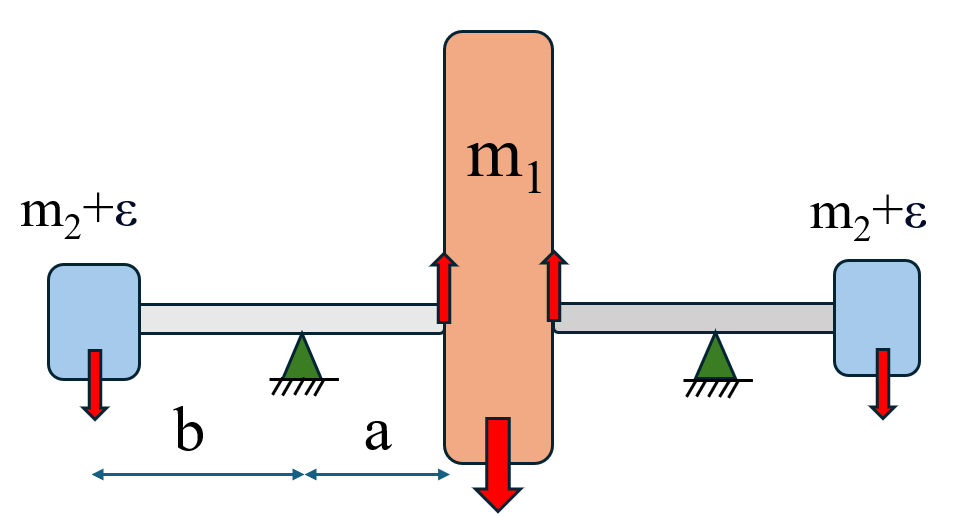
\includegraphics[width=0.6\linewidth]{images/erreur_masse.png}
    \caption{Schéma de l'axe Z avec $m_2 + \epsilon $}
    \label{fig:erreur_z}
\end{figure}
\subsubsection*{Accélération selon l'axe xy}

Supposons une accélération selon l'axe $x$ : $\vec{a_\text{cc}}$. Dans un mécanisme idéal, les centres de masse seraient parfaitement positionnés sur les pivots, et une accélération horizontale n'aurait aucun impact sur la mesure.

Cependant, considérons maintenant un léger décalage du centre de masse de la masse la plus lourde $m_1 = 0{,}191~\text{kg}$. Ce décalage, noté $\delta $, engendre une force parasite lors d'une accélération horizontale:
$$\vec{F_\text{err}} = \frac{m_1\vec{a_\text{cc}} \delta l_2}{l_1l_3}$$
Ce qui nous donne avec une accélération de $a_\text{cc} = 6 \ m/s^2$ et $ \delta = 1 mm$:
$$F_\text{err} = 4mN\Rightarrow\Delta x_\text{err} = \frac{{F_\text{err}}}{k_{\text{eq xy}}} = \frac{0,004}{4,92} \approx 0,0008 \ mm \Rightarrow \frac{\Delta x_\text{err}}{x_\text{tot}} = 0,08\%$$

\begin{figure}[H]
    \centering
    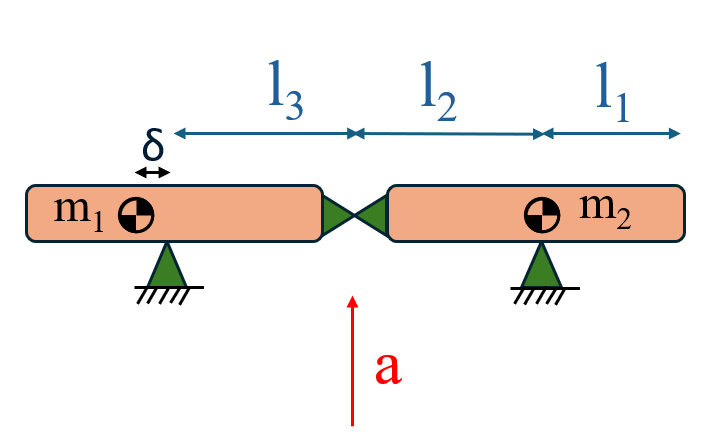
\includegraphics[width=0.6\linewidth]{images/erreur_acceleration_x.png}
    \caption{Schéma de l'axe x avec un $\delta $ sur le centre de masse}
    \label{fig:erreur_z}
\end{figure}
\subsection{Erreur de mesure de force induites par les changement d’orientation de la gravité}

Lorsque l'orientation du mécanisme change dans l’espace, la direction du vecteur gravité dans le repère du palpeur est modifiée. En particulier, si le palpeur est incliné d’un angle $\alpha$ par rapport à la verticale, l’accélération gravitationnelle se décompose selon les axes $x$ et $z$ comme suit :
\[
\vec{g} = g \left( \sin(\alpha)\hat{x} + \cos(\alpha)\hat{z} \right)
\]
Des sections précédentes on obtient:
$$\vec{F_\text{err}} = \epsilon_m\frac{b}{a}\vec{a_\text{ccz}} + \frac{m_1 \delta l_2}{l_1l_3}\vec{a_\text{ccx}} = \epsilon_mg\cos(\alpha)\frac{b}{a}\hat{z} + \frac{m_1g\sin(\alpha) \delta l_2}{l_1l_3}\hat{x}$$
Ce qui nous donne avec une alpha de $20^\circ$ et les même approximations qu'avant:
$$\vec{F_\text{err}} = 0,008\hat{z} + 1,7\times10^{-6}\hat{x} \approx 0,008\hat{z} \Rightarrow\Delta x_\text{err} = \frac{{F_\text{err}}}{k_{\text{eq}_Z}} = \frac{0,008}{5,28} \approx 0,0015 \ mm \Rightarrow \frac{\Delta x_\text{err}}{x_\text{tot}} = 0,15\%$$

  


\subsection{Erreur de mesure de force induite par les accélérations en rotation}\label{sub:bonecaambalabu}
\subsubsection*{Erreur sur le centre de masse}
Calculons maintenant l'erreur dûe à une accéleration angulaire. En effet, nous avions fait l'hypothèse dans la section \ref{sub:labelito} que les centres de masses et de rotation étaient confondus. Analysons l'erreur de mesure en cas de distance $\delta$ entre le centre de rotation et le centre de masse Posons donc la somme des moments, en utilisant la règle de Steiner:

$$\vec{M_\text{err}} = I_1\vec{\alpha_\text{1}} - (I_2 +
 m_2\delta^2)\vec{\alpha_\text{2}} = -
 m_2\delta^2\vec{\alpha_\text{2}}$$

 De là, on peut donc déduire la force parasite:

 $$\vec{M_\text{err}} =\vec{F_\text{err,xy}}l_\text{1} \Rightarrow F_\text{err} = \frac{
 m_2\delta^2{\alpha_\text{2}}}{l_\text{1}} $$

 Comme on a $k_{\text{eq}_{x,y}}$ en translation du stylet, on en déduit le déplacement parasite  $\Delta x_\text{err}$ pour un moment d'inertie pour $m_\text{2}=0.117$ $kg$, une erreur de $\delta = 1mm$, une accélération de $\alpha$ = 30 $rad/s^2$ $I_{\text{2}_{x,y}}\approx71$ $kg\cdot mm^2$.

 $$F_\text{err} \approx 0,015mN \Rightarrow \Delta x_\text{err} = \frac{{F_\text{err}}}{k_{\text{eq}_Z}} =\frac{1,5\times10^{-5}}{4.9}\approx 3,1\times 10^{-6} \ mm \Rightarrow \frac{\Delta x_\text{err}}{x_\text{tot}} \approx 0,0003 \% $$



 \begin{figure}[H]
    \centering
    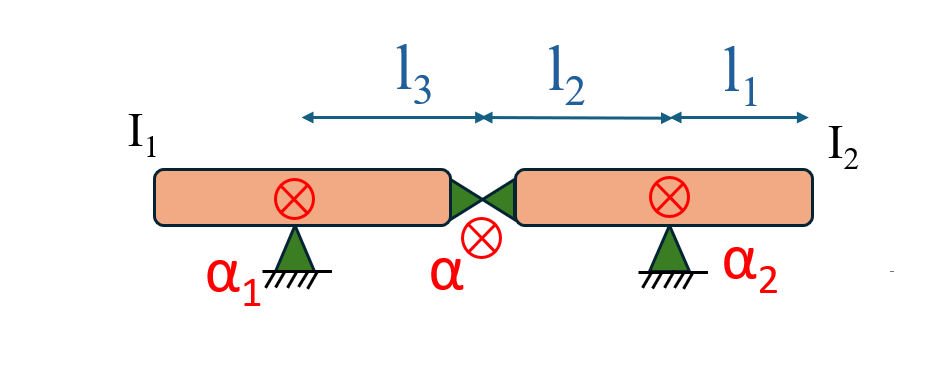
\includegraphics[width=0.6\linewidth]{images/erreur_rotation_xy.png}
    \caption{Schéma de l'axe x avec accélération $\alpha$ selon y}
    \label{fig:erreur_xy_rotation}
\end{figure}
\subsubsection*{Erreur sur l'inertie}
Nous ajoutons un $\psi$ d'erreur sur I:

$$\vec{M_\text{err}} = I_1\vec{\alpha_\text{1}} - (I_2 + \psi I_2)\vec{\alpha_\text{2}} = -\psi I_2\vec{\alpha_\text{2}}$$
Nous pouvons en déduire la force parasite: 
$$\vec{M_\text{err}} =\vec{F_\text{err,xy}}l_\text{1} \Rightarrow F_\text{err} = \frac{
 \psi I_2\alpha_2}{l_\text{1}} $$
 
Avec (valeur directement récupérée dans la modélisation 3d) $I_2 = 71kgmm^2$ et une erreur de $1g$ sur la masse nous donne $I_2 = cm_2, \ I_2'=c(m_2 + 1g)$ $ \Rightarrow \Delta_I = \psi I_2 \approx 0,6 kgmm^2 $. la force vaut donc:

 $$F_\text{err} \approx 0,014mN$$



 
\subsection{Erreur de mesure de force induite par les vitesses angulaires}

Supposons maintenant une rotation angulaire $ \omega $ autour de l’axe $z$, et analysons l’erreur de mesure, à travers la force centrifuge induite. Comme illustré sur la figure \ref{fig:erreur_z_rotation}, le système comprend deux masses $m_2$ situées à une distance $a+b$ de l’axe de rotation.

Nous arrivons donc à une force induite de:
$$F_\text{err z}=2\sin{\beta}\cdot F_c \  \text{, avec} \ F_c = m_2a_C  = m_2\frac{v^2}{a+b} = m_2\omega^2\cdot (a+b)$$

Avec un angle $\beta_\text{max} = 6^\circ$ et $\omega = 5 \text{ rad/s}$ nous arrivons à une erreur max de:
$$\Rightarrow \Delta x_\text{err} = \frac{{F_\text{err}}}{k_{\text{eq}_Z}} = \frac{0,014}{5,28} \approx 0,003\mathrm{mm} \Rightarrow \frac{\Delta x_\text{err}}{x_\text{tot}} = 0,3\% $$

\begin{figure}[H]
    \centering
    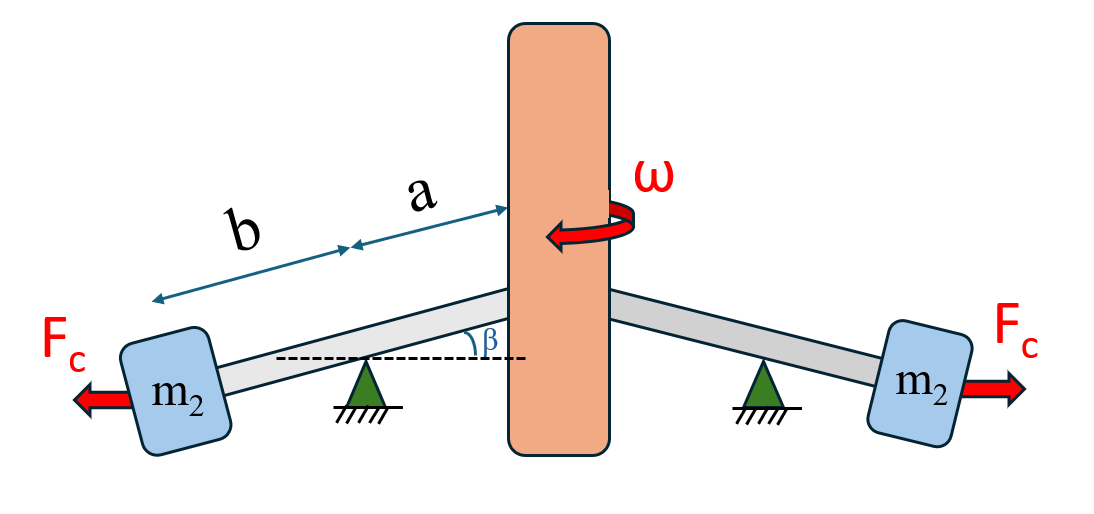
\includegraphics[width=0.6\linewidth]{images/erreur_rotation_z.png}
    \caption{Schéma de l'axe Z avec rotation $\omega$}
    \label{fig:erreur_z_rotation}
\end{figure}

\subsection{Discussion des erreurs de mesure}
Nous avons donc estimé et calculé les erreurs de mesure dûes à plusieurs inexactitudes entre le modèle réel et le modèle théorique. Les plus grandes forces fictives que nous avons trouvées valent 14 $mN$. Cela est raisonnable et correspond au cahier des charges, car inférieur à 15 $mN$. Ces forces sont donc bien négligeables dans les calculs et  n'entravent pas le bon fonctionnement du système.

Cependant certaines approximations que nous avons faites sont faible et dur à obtenir dans la réalité. C'est principalement le cas de $\epsilon_m$. Dans le prolongement du projet nous pourrions imaginer des masses plus volumineuse mais avec une densité plus faible pour pouvoir nous approcher le plus possible de cette erreur.Nous pouvons donc voir que nos erreurs restent toutes en-dessous de 2\%, et que le système marche sans que les imprécisions mentionnées ci-dessus n'entravent son fonctionnement. 

\subsection{Erreur de mesure de force induite par les non-linéarités du corps d’épreuve}
Dans notre conception, nous avons fait l'hypothèse des petits déplacements. Cette hypothèse s'applique très bien dans le cadre ne notre projet car les courses de nos articulations restent bien en deçà de leurs courses admissibles, minimisant ainsi les effets dûs à la non linéarité qui sont surtout observés en fin de course ou lors de déformation importantes. L'erreur de mesure induite par la non linéarité de rigidité est donc négligeable. 
\\De la même manière, des défauts de non-linéarité d'inertie peuvent être observés.  Ces derniers peuvent apparaître dans des cas d'utilisation dynamique lorsque la géométrie du mécanisme est modifiée par la mesure d'une force. Une fois encore, nos déplacements sont très petits (pour plus de détails, voir section \ref{cinématique}). Ces défauts sont minimes et donc négligés dans nos calculs. Une validation expérimentale (sur un prototype dans une prochaine phase de développement, par exemple) permettrait de quantifier ces erreurs potentielles dûes à ces non-linéarités et d'identifier les éventuelles limites des simplifications.



\section{Discussion}
\subsection{Tableau des conformités avec le cahier des charges}
\begin{table}[H]
\centering
\renewcommand{\arraystretch}{1.4} % Hauteur des lignes
\begin{tabularx}{\textwidth}{|>{\raggedright\arraybackslash}p{3.5cm}|>{\raggedright\arraybackslash}X|>{\raggedright\arraybackslash}X|}
\hline
\textbf{Thème} & \textbf{Objectif du cahier des charges} & \textbf{Réalisation} \\
\hline
Encombrement $\star$  & Hauteur max de 191 mm, diamètre max de 84 mm & Hauteur : 191 mm, diamètre : 80mm non sollicité, 81.7 mm au pire des cas\\
\hline
Masse $\star$ & Masse du capteur : 1 kg & Masse totale mesurée à 978g, châssis, vis et capteurs compris  \\
\hline
Mesure force $\star$ & Plage de mesure de la force : ±5 N & Respectée, avec butées pour ±5,5 N \\
\hline
Mesure du déplacement $\star$ & Plage de mesure du déplacement : ±1 mm & Amplitude conforme avec capteur à 1 mm \\
\hline
Rigidité $\star$ & Rigidité 5 N/mm (± 0.5)& Rigidité équivalente obtenue : ±5,28 N/mm selon z et ±4,92 N/mm selon xy \\
\hline
Résolution de mesure de la force $\star$ & Résolution $\leq$ 1.5 mN & ±0.11 mN atteinte sur X/Y, 0.41 mN sur Z \\
\hline
Inertie $\star$ & Erreur due à l'inertie < 15 mN & ± 14mN au pire des cas \\
\hline
Corps d'épreuve en guidages fléxibles. $\star$ & 3 DDL en guidages flexibles & Mécanisme avec aucun frottement solide et sans ressorts ajoutés \\
\hline
Équilibrage forces $\star$ & Insensibilité à la gravité et translation de la base & Mécanisme équilibré en forces\\
\hline
Équilibrage en moments $\star$ & Insensibilité aux accélérations en rotation & Mécanisme équilibré en moments \\
\hline
Invariance inertielle & Insensibilité aux vitesses angulaires &  Mécanisme sensible au vitesses angulaires \\
\hline
Solidité & Résistance à ±15 N sans endommagement & Système de butées garantissant le confinement du déplacement dans les limites admissibles\\
\hline
Durée de vie & >10 ans à 2 Hz, 4h/jour & $\sigma_{\text{max}} << \sigma_{\text{D}}$ : casi-insensibilité à la fatigue\\
\hline
Température & Fonctionnement : 23 ± 5°C & Propriétés du matériau prises pour environ 23°C\\
\hline
Coût & < 300 CHF (indicatif) & Coût supérieur selon nous, malgré l'absence d'assemblage du corps principal \\
\hline
\end{tabularx}
\caption{Résumé des exigences du cahier des charges et leur réalisation}
\end{table}
\subsection{Justification des non conformités du cahier des charge et impacts}
Le mécanisme présenté respecte tous les critères déterminants du cahier des charges. \\
L'atteinte de l'invariance inertielle aurait nécessité une mise en symétrie dynamique des masses en mouvement, l'ajout de nouvelles masses ou encore de nouvelles structures, ce qui aurait fortement compromis les autres points du cahier des charges que nous avons préféré prioriser (encombrement, masse totale, etc). Ce critère a donc été assez tôt volontairement écarté au profit d'un système plus simple et plus compact.\\
Les contraintes d'encombrement nous ont conduit à concevoir un design se comportant différemment selon l'axe Z et les axes X-Y, ce qui nous a amené à avoir une légère différence de rigidité entre ceux-ci. Cette différence a été minimisée au maximum et est relativement faible ($\approx$0,35 $N/mm$, voir section \ref{rigidite}).
Le dépassement budgétaire indicatif est justifié par le choix d'un système monolithique et précis. Les calculs exacts des coûts n'ont pas étés effectués mais nous semblent peu atteignables en utilisant l'électroérosion à fil (voir \ref{sub:construction} pour les détails de ce choix ainsi que des pistes pour réduire ce coût). Le coût élevé du dispositif peut également se justifier par la large marge de sécurité offerte par notre conception. En effet, les contraintes mécaniques restent très en dessous des limites admissibles, ce qui garantit une durée de vie extrêmement élevée, bien au-delà des 10 ans exigés. Le mécanisme présente ainsi une grande robustesse et ne nécessite aucun remplacement à long terme, ce qui compense en partie le surcoût initial.




\section{Construction}
\label{sub:construction}
\subsection{Choix de construction}
\label{choix_construction}
Nous avons choisi de créer une pièce monobloc, dont les principaux avantages sont l’élimination des hyperstatismes liés aux tables à lames parallèles et aux doubles-pivots (rotule), ainsi que la réduction des coûts d’assemblage. Pour cela, nous avons choisi d'usiner notre pièce en électroérosion à fil, qui permet d'usiner des lames avec précision.\\

La fabrication se fera en deux étapes : un premier en usinage par fraisage, en retournant la pièce, suivi d’une finition par électroérosion à fil pour tous les éléments flexibles.
Nous avons à cette fin conçu un brut d’usinage en forme de rectangle, le plus fin possible tout en respectant l’encombrement, afin de limiter le gaspillage de matière malgré la nature monobloc de la pièce. \\

L'usinage par électroérosion a nécessité une adaptation de notre design pour garantir un accès libre selon les axes X et Y au niveau des zones à usiner, comme illustré en exemple dans la figure \ref{fig:electroeriosion}.C'est également pour cette raison que nous avons choisi d'utiliser des pivots à lames croisées non séparées plutôt que séparées, ce qui a été facilité par le fait que notre design ne demande que de faibles courses angulaires au niveau des pivots.\\ 

Il faudra ainsi électro-éroder la pièce une fois selon l'axe X et une fois selon l'axe Y. Les tables à lames parallèles nécessitent d'utiliser un pont par lame, car la longueur de celles ci est supérieur à $60 \cdot h$.
Notre design offre par ailleurs la possibilité d'être usiné en plus grande quantité si les pièces sont mises en parallèle et que le fil traverse 2 pièces ou plus en même temps, permettant ainsi une réduction du prix de production à la chaîne. Toutefois, les aspects techniques et pratiques de cette solution n’ont pas été examinés en profondeur dans cette première phase du projet, mais pourraient l'être par la suite afin de réduire le coût par pièce.\\

Le châssis, composé de deux pièces (une pour fixer le palpeur au bâti et une pour pouvoir fixer les capteurs), ainsi que les masses seront usinés de manière classique. Pour le châssis, un tolérancement ISO 2768-m convient, hormis pour la distance entre les 2 branches de celui-ci qui doit être plus précise. Pour ce qui est des masses, une grande précision d'usinage sera nécessaire (voir section \ref{sub:erreur_mesure})

Enfin, nous avons décidé de séparer les contrepoids de la pièce principale de sorte qu'ils soient  amovibles afin de pouvoir choisir une densité plus élevée ainsi que pour faciliter l'équilibrage en cas de changement de masse ou de taille du stylet.


\begin{figure}[H]
    \centering
    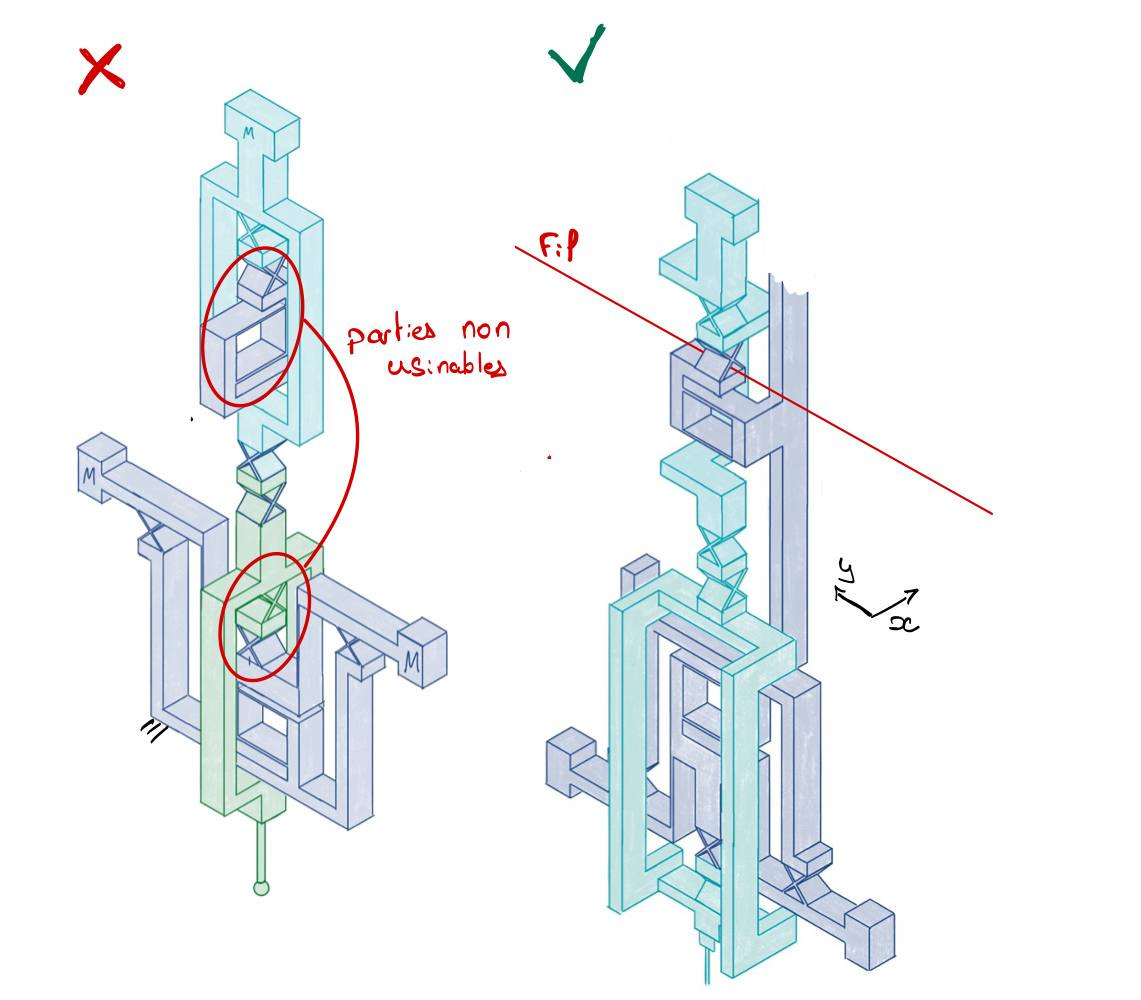
\includegraphics[width=0.75\linewidth]{images/electroeriosion.jpg}
    \caption{Adaptation du design pour l'usinage}
        \label{fig:electroeriosion}
\end{figure}


\subsection{Argumentation des choix des matériaux}
Le choix du matériau pour la pièce principale dépend principalement du module de Young, qui influence la rigidité des éléments flexibles.

Le recours à l’électroérosion imposait l’usage d’un matériau métallique conducteur. En effet, ce procédé nécessite un matériau conducteur pour fonctionner.

Nous avons également consulté le logiciel CES EduPack utilisé en cours de matériaux, en tenant compte du fait qu’un guidage flexible nécessite un matériau à module de Young élevé et avec une bonne élasticité pour supporter de grandes déformations répétées. Les principaux matériaux répondant à ces critères sont : l’acier, les alliages de nickel et le titane.

Pour des raisons de coût, le titane a été écarté. Nous avons choisi l’acier, un matériau courant, facile à usiner et compatible avec l’électroérosion.

Les masses séparables sont en plomb, un matériau que nous avons choisi pour sa densité élevée




\section{Conclusion et perspectives}

Le projet FlyForce a permis de concevoir un mécanisme de mesure de force reposant uniquement sur des guidages flexibles, sans pièces mobiles traditionnelles, ni frottement, ni jeu mécanique. Nous avons dans cette première phase de développement validé le principe de fonctionnement du mécanisme, réalisé une conception détaillée et mené un dimensionnement complet en adéquation avec le cahier des charges. Cette première phase pose les bases d’une conception avancée de notre palpeur, ainsi que de la réalisation d’un prototype. Une amélioration envisagée serait d'allonger les courses angulaires  des pivots flexibles dans le but d'amplifier les déplacements mesurables, mais il faudrait pour cela trouver des capteurs capables de mesurer un déplacement angulaire supérieur à 1°, ou encore transformer le mouvement de rotation en mouvement de translation au niveau des points de mesure. Il serait également intéressant d'améliorer l'isotropie de notre mécanisme, ou à défaut, de prendre en compte cette anisotropie dans le traitement des données des capteurs. Par ailleurs, une analyse plus poussée des coûts de fabrication serait nécessaire, en étudiant notamment la simplification des pièces ou le recours à des procédés de fabrication plus économiques, afin de rendre le système plus facilement industrialisable.



\section{Annexes} \label{Annexes}
\subsection{Maquette}
Nous avons réalisé une maquette pour mieux comprendre la cinématique de notre palpeur en implantation flexible. Elle est à l’échelle 1:1, avec une conception simplifiée afin de faciliter son impression en 3D et son assemblage à l’aide de lames en acier inoxydable (un matériau proche de celui utilisé dans la conception finale). Les lames utilisées ont une épaisseur de 200µm, ce qui ne correspond pas exactement aux épaisseurs réelles (comprises entre 60 et 450µm), mais offre néanmoins une bonne approximation du comportement mécanique.

On observe que le déplacement selon l’axe Z est nettement plus rigide que les rotations autour des axes X et Y. Cette différence est due à l’épaisseur des lames et des pivaux latéraux qui est supérieure à celle prévue pour le mécanisme final, ainsi qu’aux pivots centraux, qui eux sont plus fins.

\begin{figure}[H]
    \centering
    
    \begin{subfigure}[b]{0.45\linewidth}
        \centering
        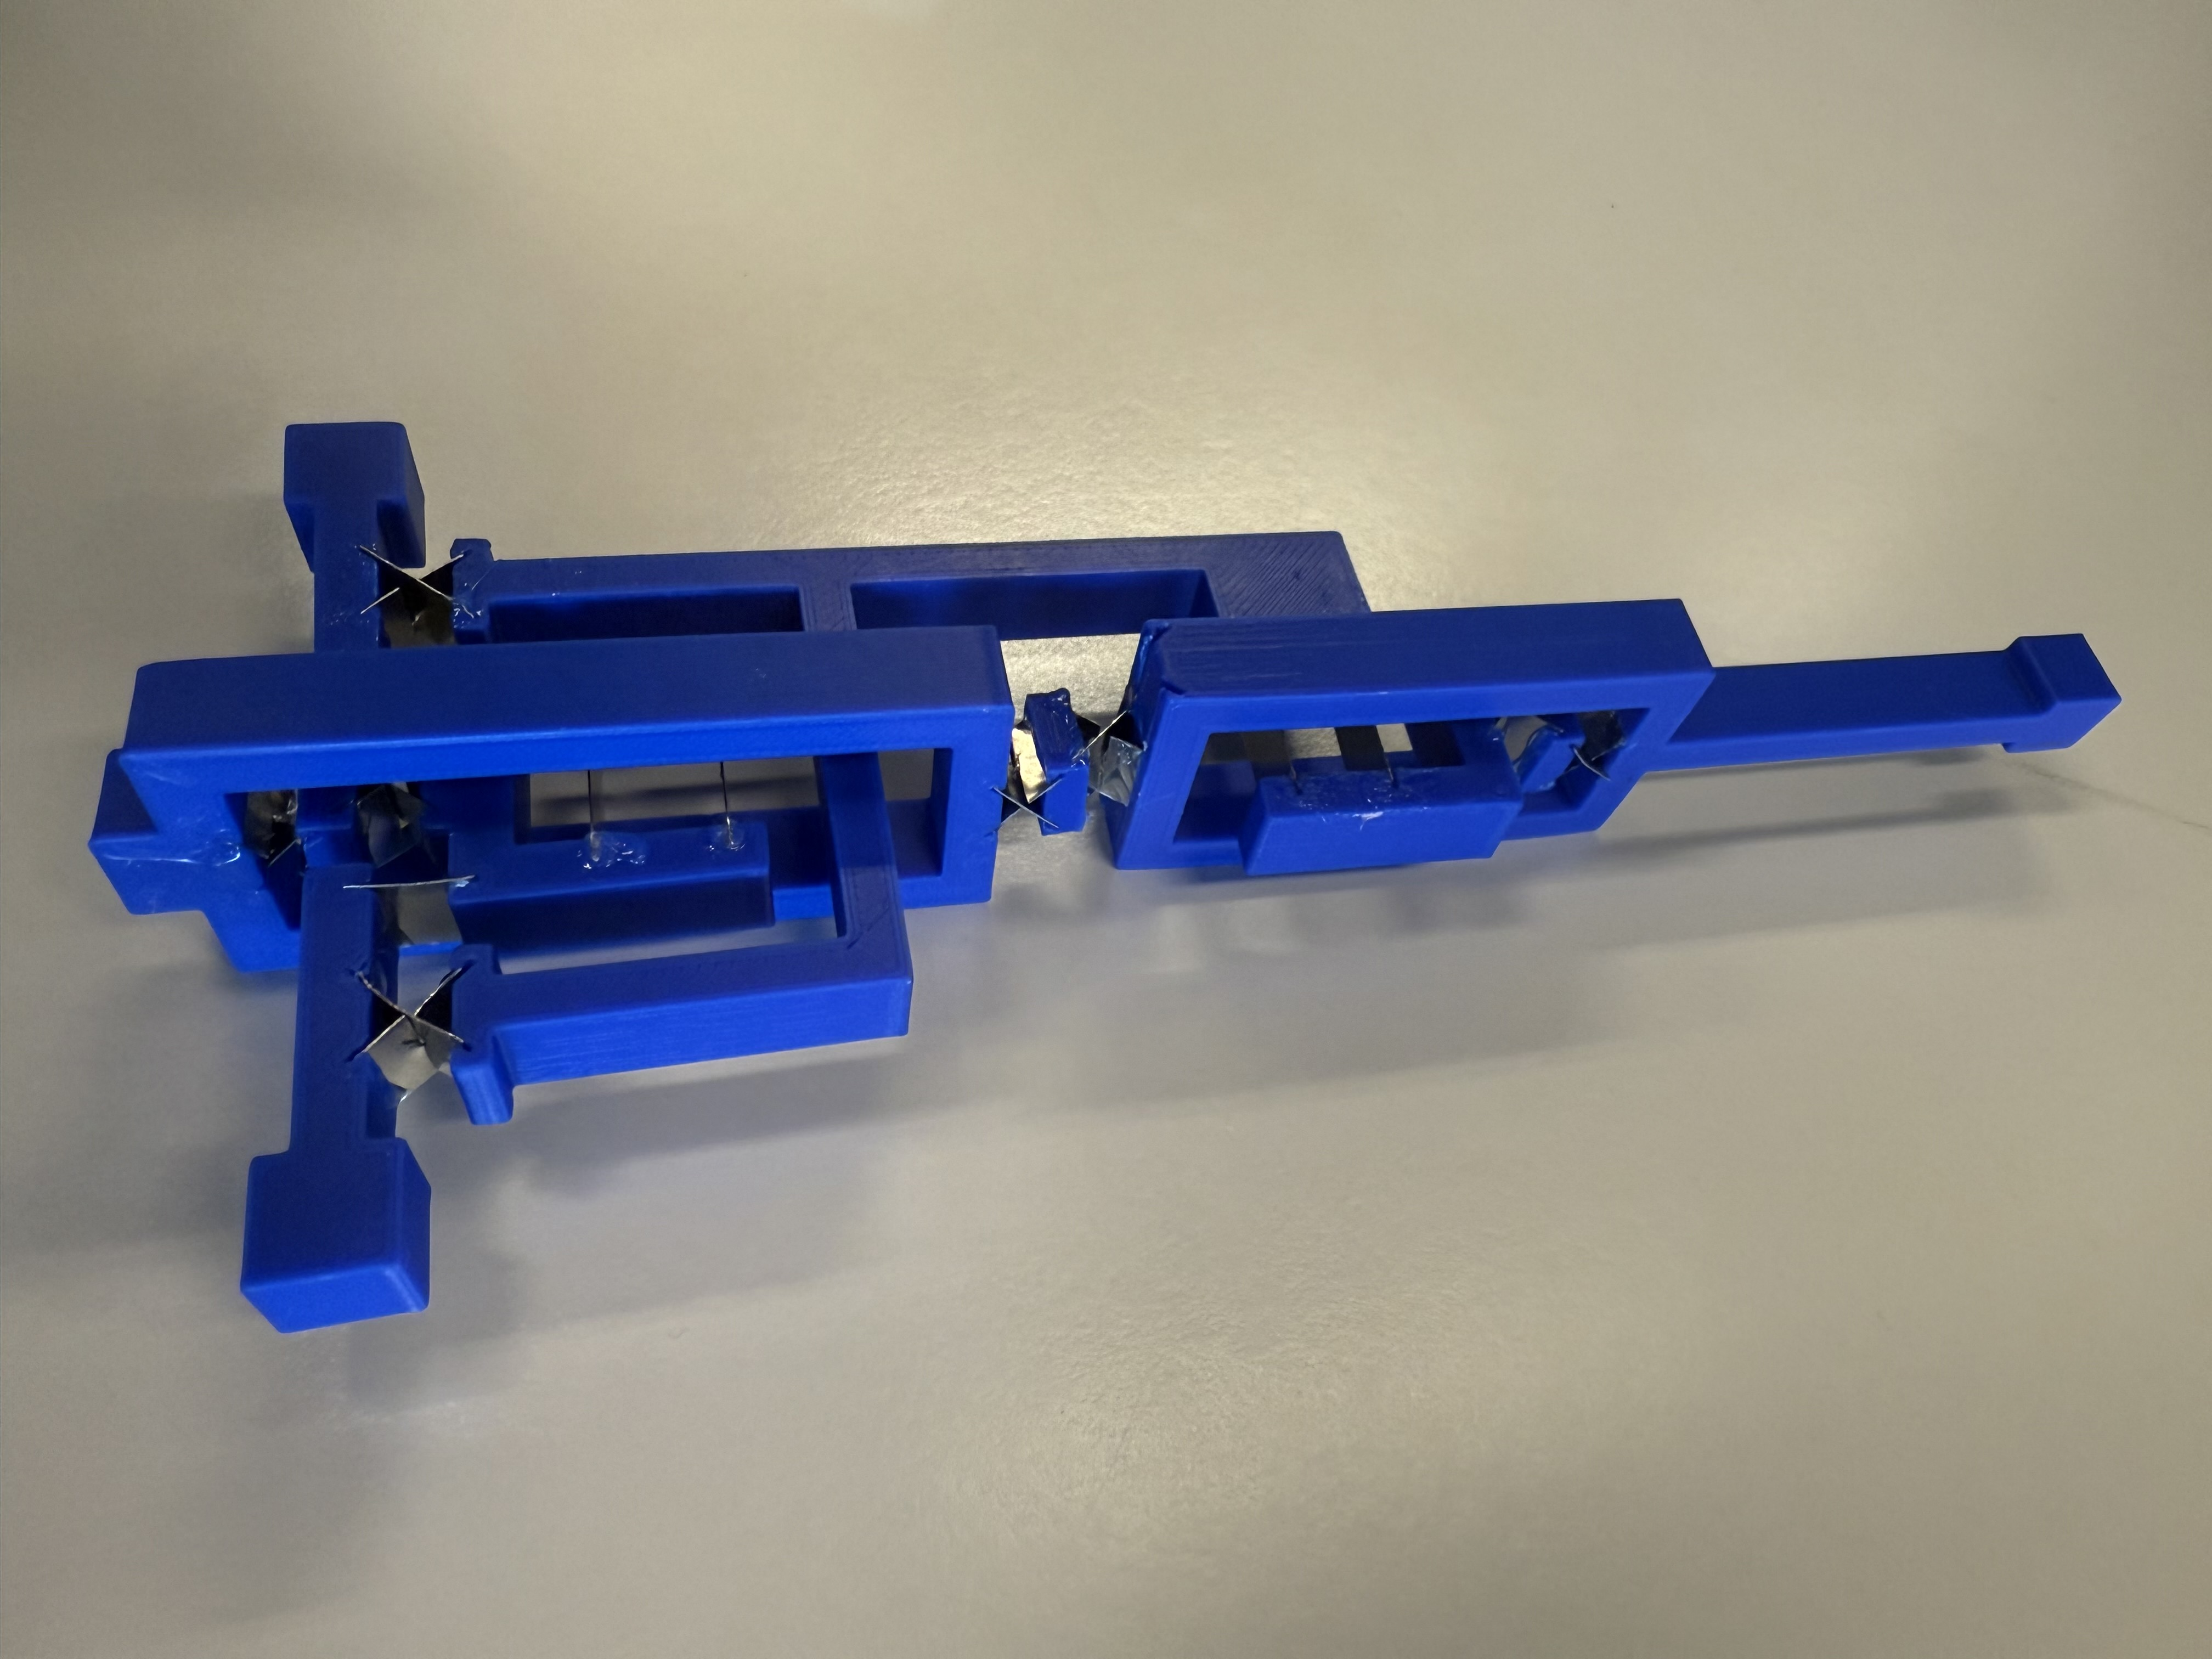
\includegraphics[width=\linewidth]{images/IMG_2560.jpeg}
        \caption{Maquette}
        \label{fig:maquette1}
    \end{subfigure}
    \hfill
    \begin{subfigure}[b]{0.45\linewidth}
        \centering
        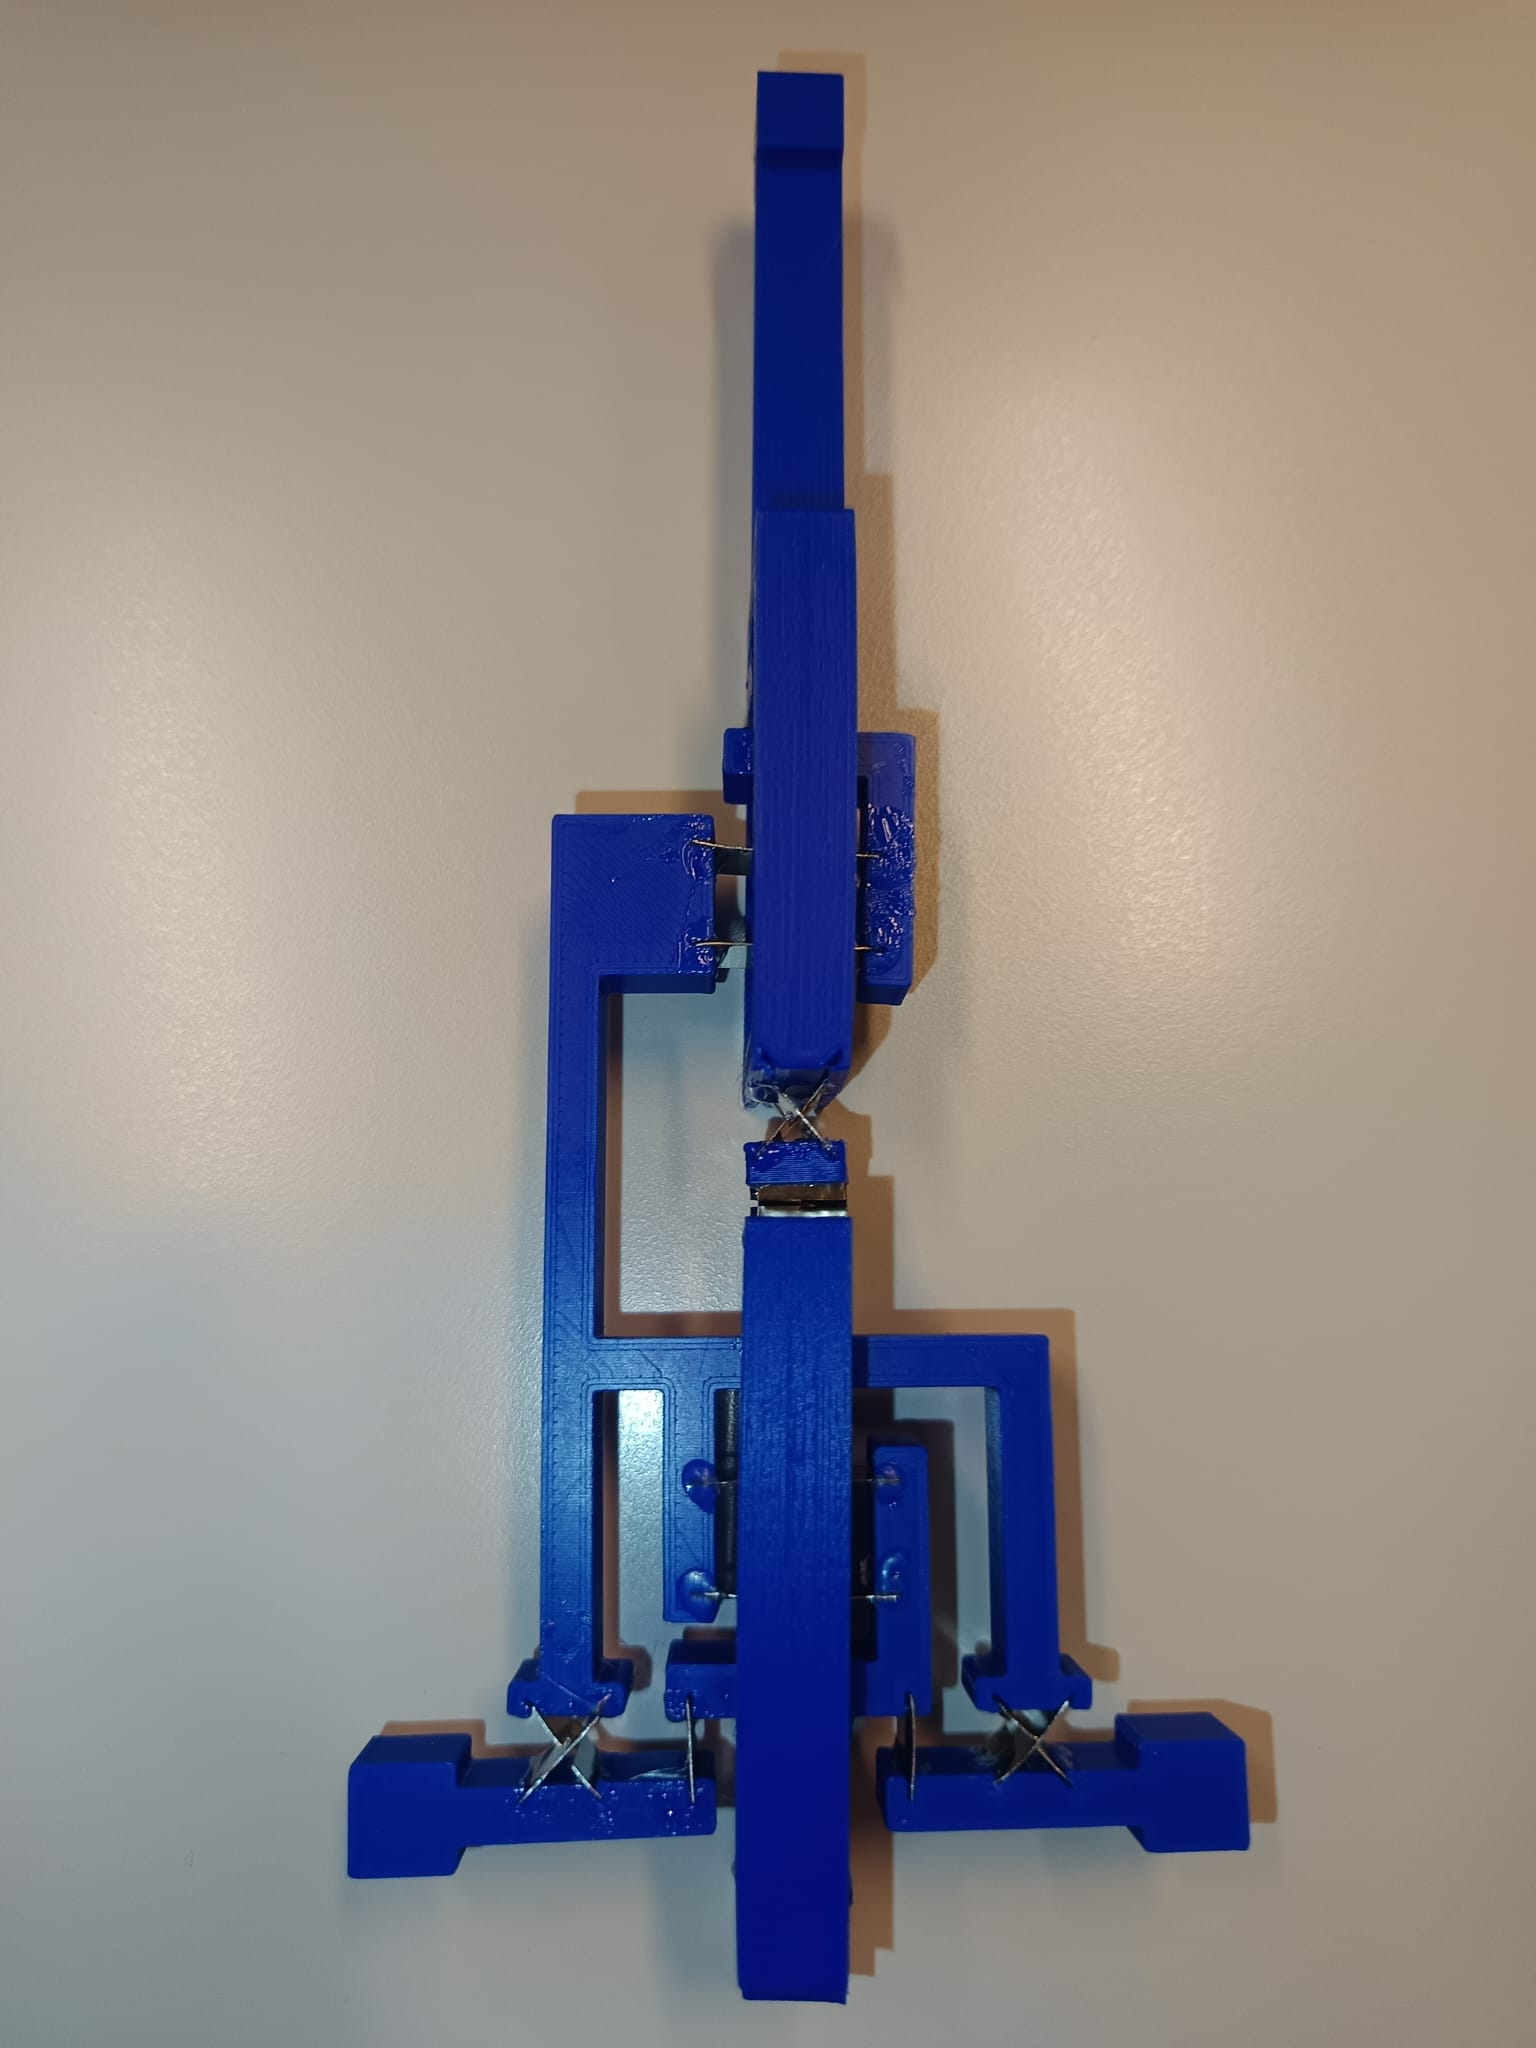
\includegraphics[width=\linewidth]{images/maquette.jpg}
        \caption{Maquette imprimée en 3D avec lames en acier inoxydable}
        \label{fig:maquette2}
    \end{subfigure}
    \vskip\baselineskip
    \begin{subfigure}[b]{0.45\linewidth}
        \centering
        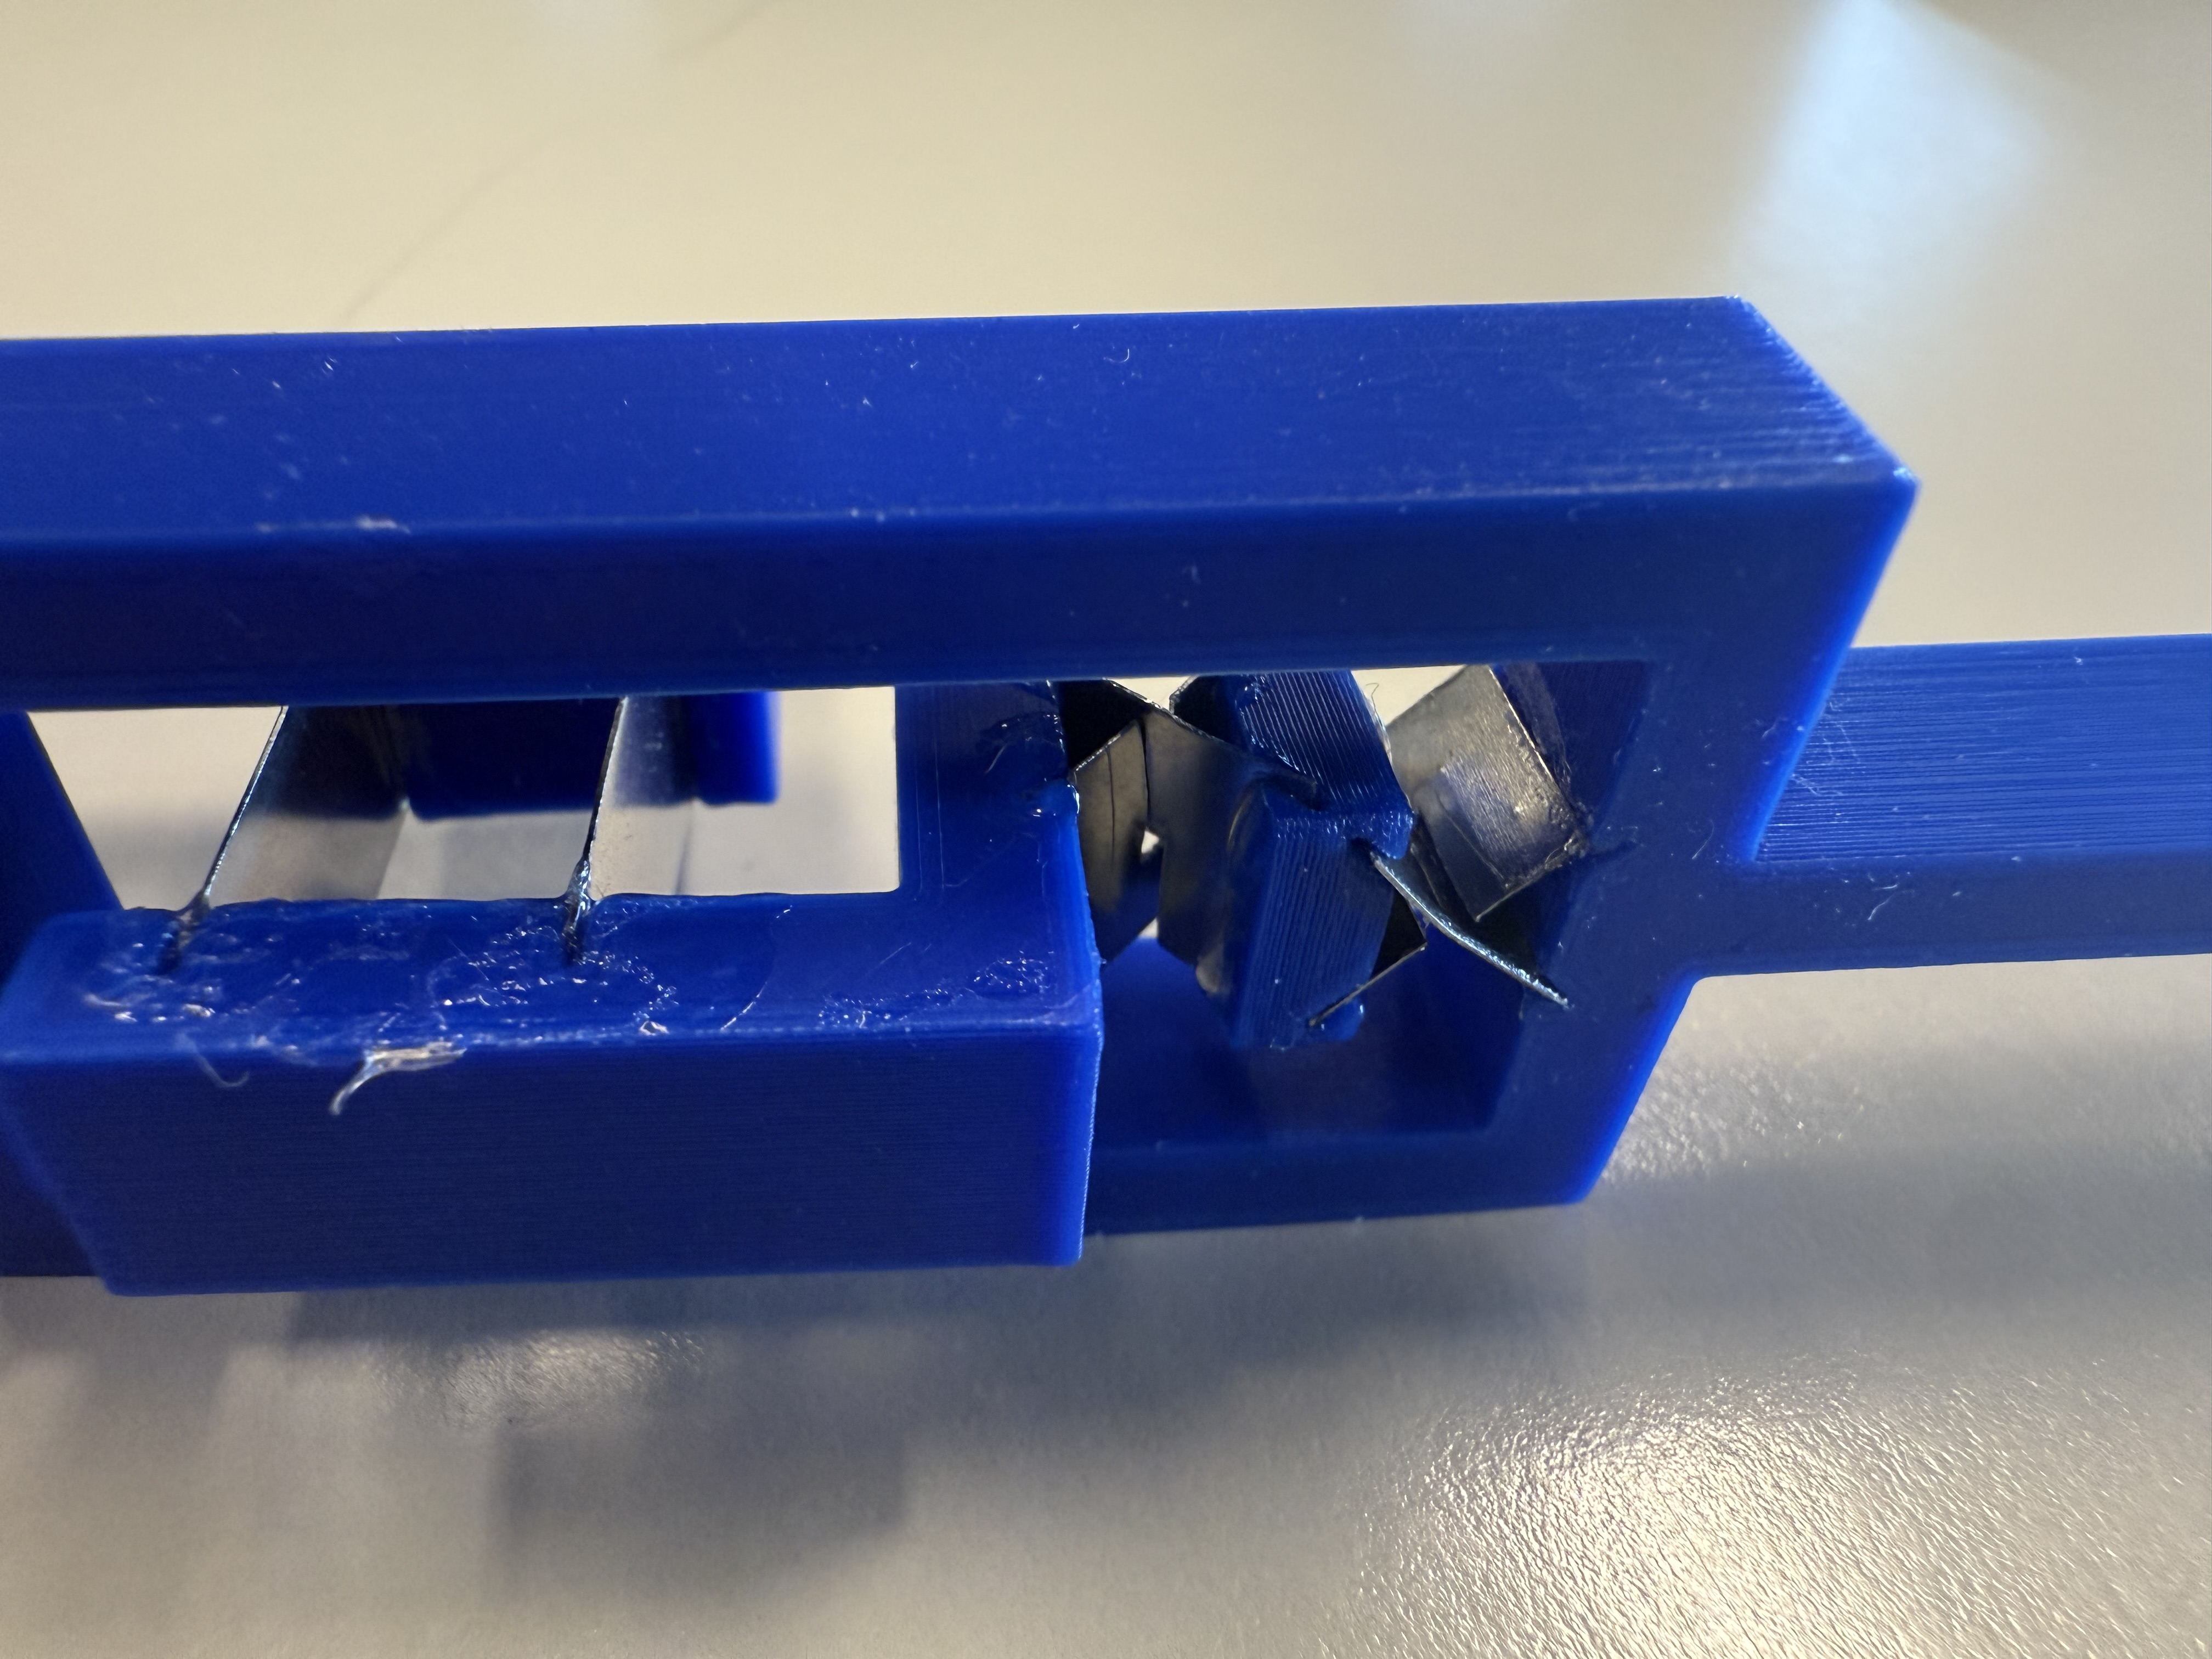
\includegraphics[width=\linewidth]{images/IMG_2562.jpeg}
        \caption{Équilibrage X et Y}
        \label{fig:equilibrageXY}
    \end{subfigure}
    \hfill
    \begin{subfigure}[b]{0.45\linewidth}
        \centering
        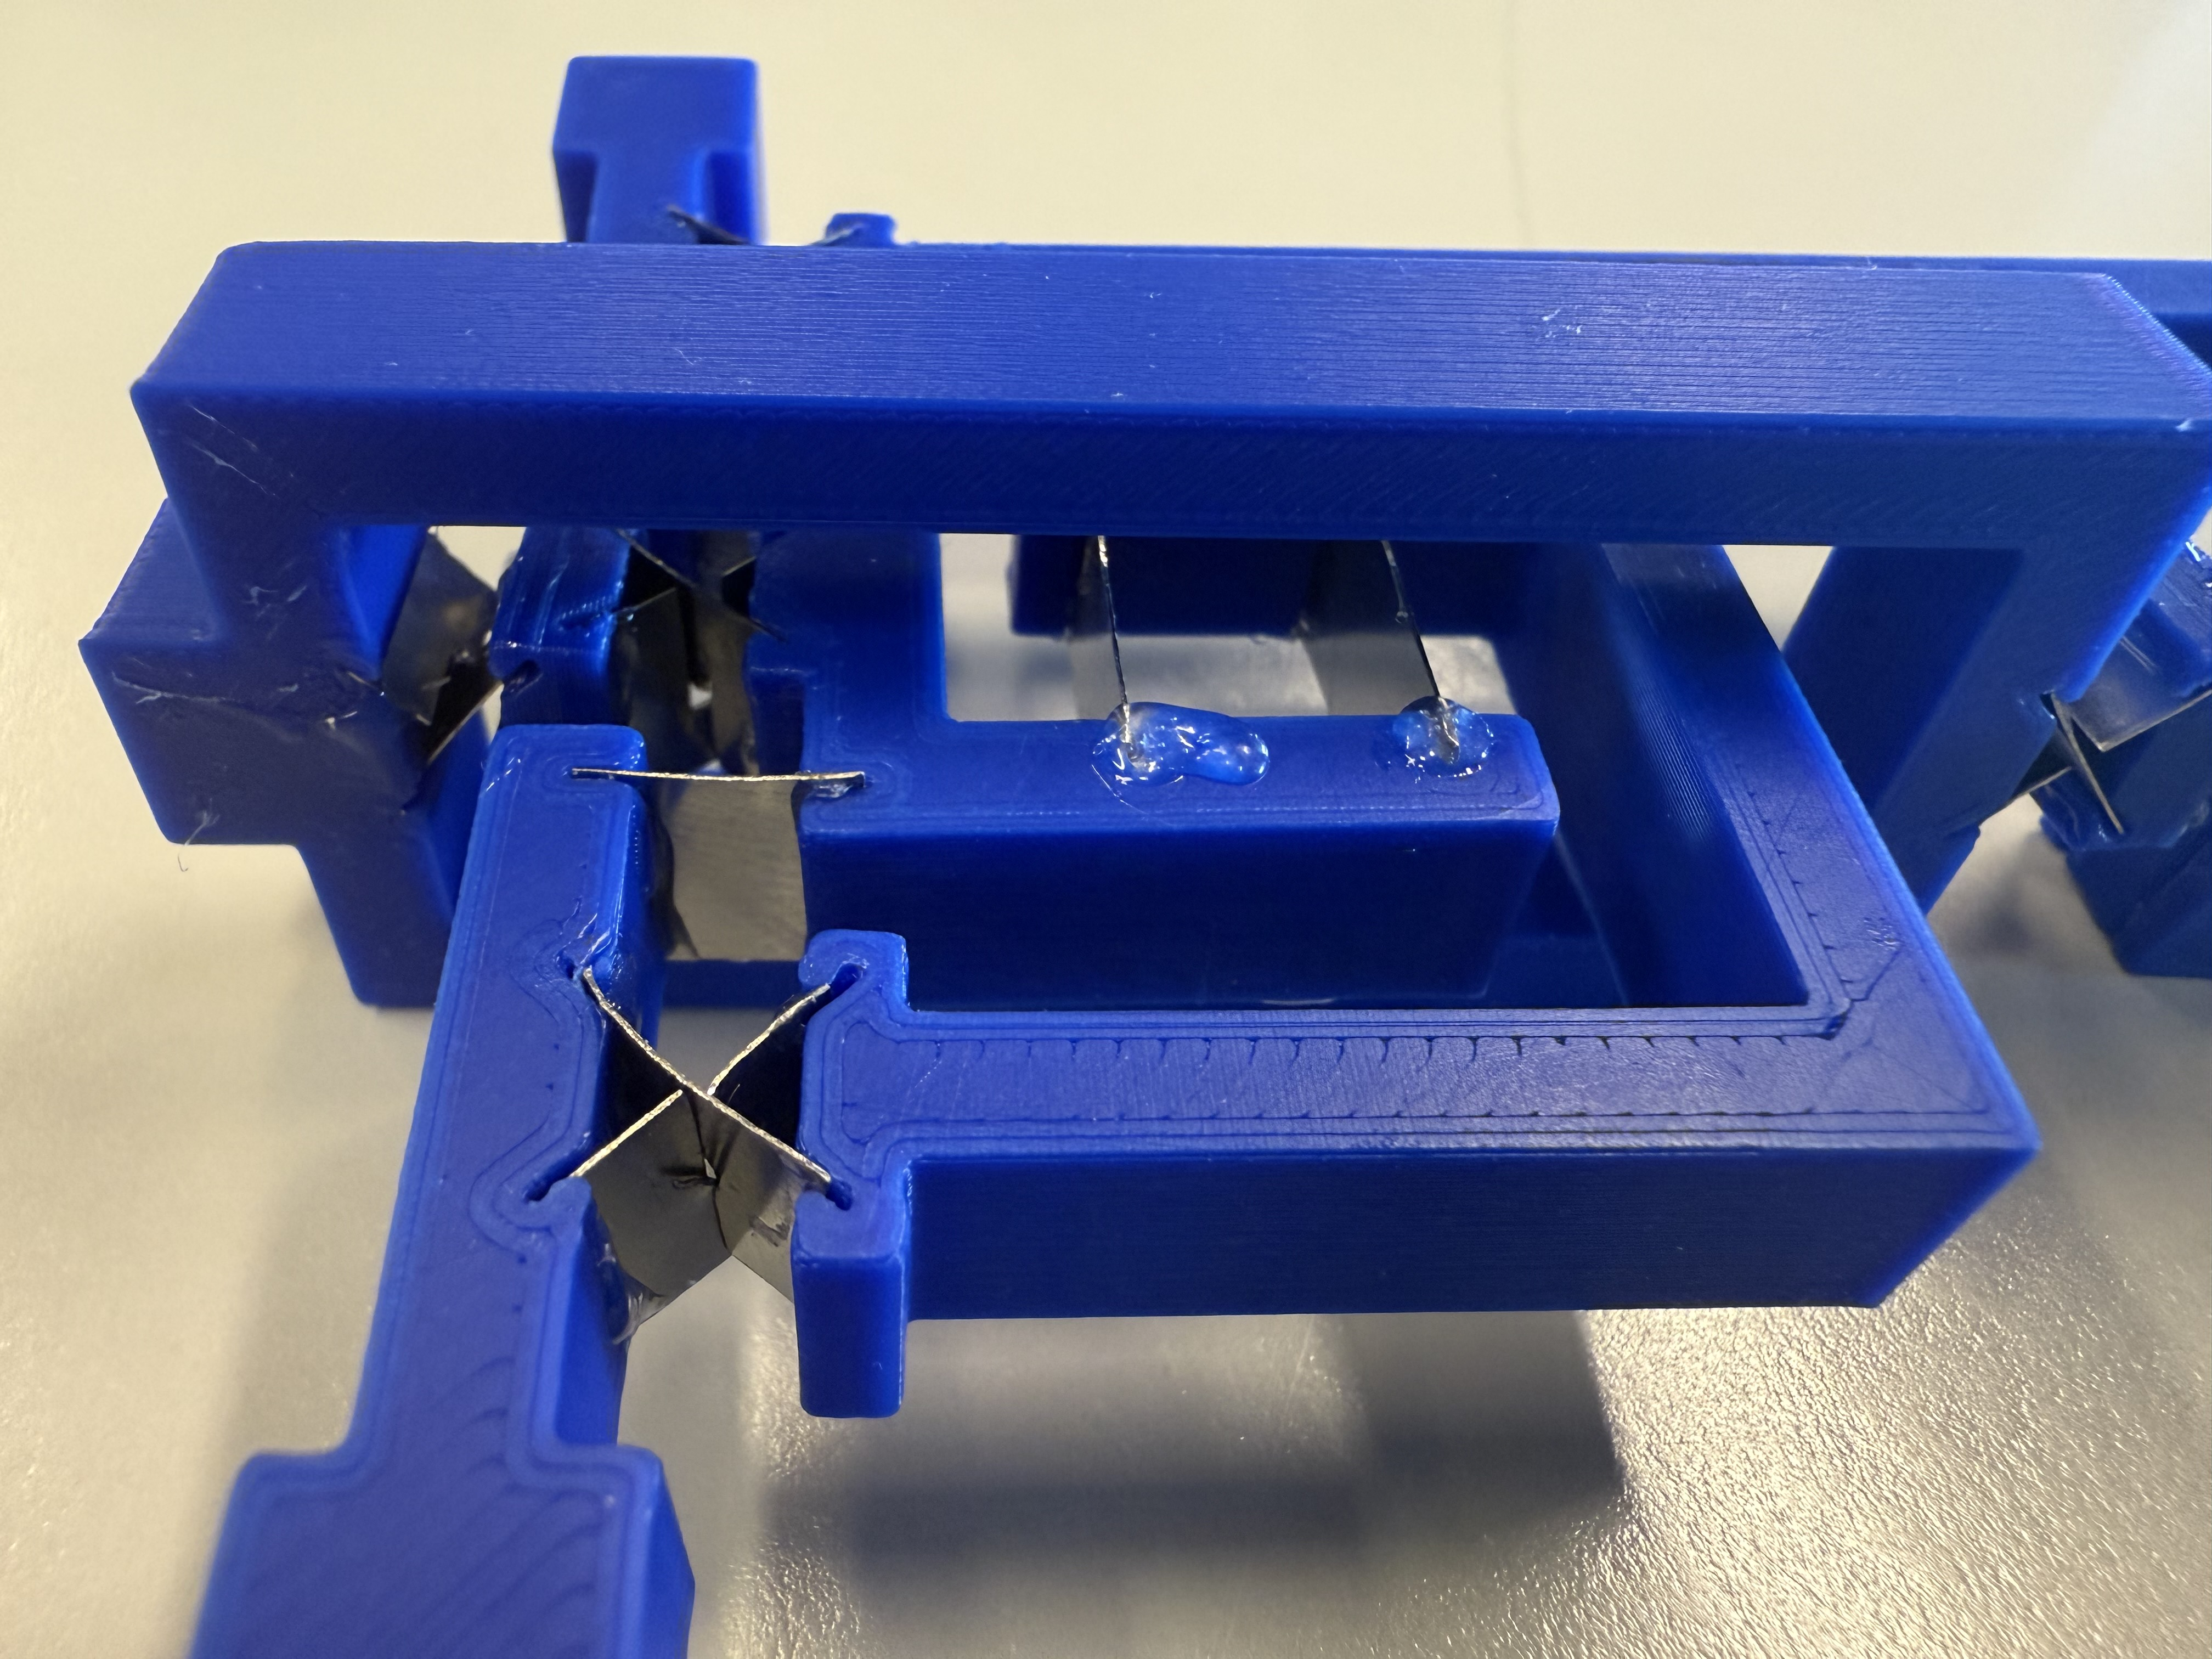
\includegraphics[width=\linewidth]{images/IMG_2561.jpeg}
        \caption{Équilibrage Z}
        \label{fig:equilibrageZ}
    \end{subfigure}
    \caption{Maquette 3D vues des équilibrage pour les axes X, Y et Z, taille réelle}
    \label{fig:maquette-carree}
\end{figure}

\newpage
\subsection{Programme d'optimisation Matlab}
\label{prog}
\lstinputlisting[language=Matlab]{Annexes/flyforce.m}

\subsection{Fichier Excel utilisé lors du dimensionnement}

\subsection{Planche et dessins techniques}

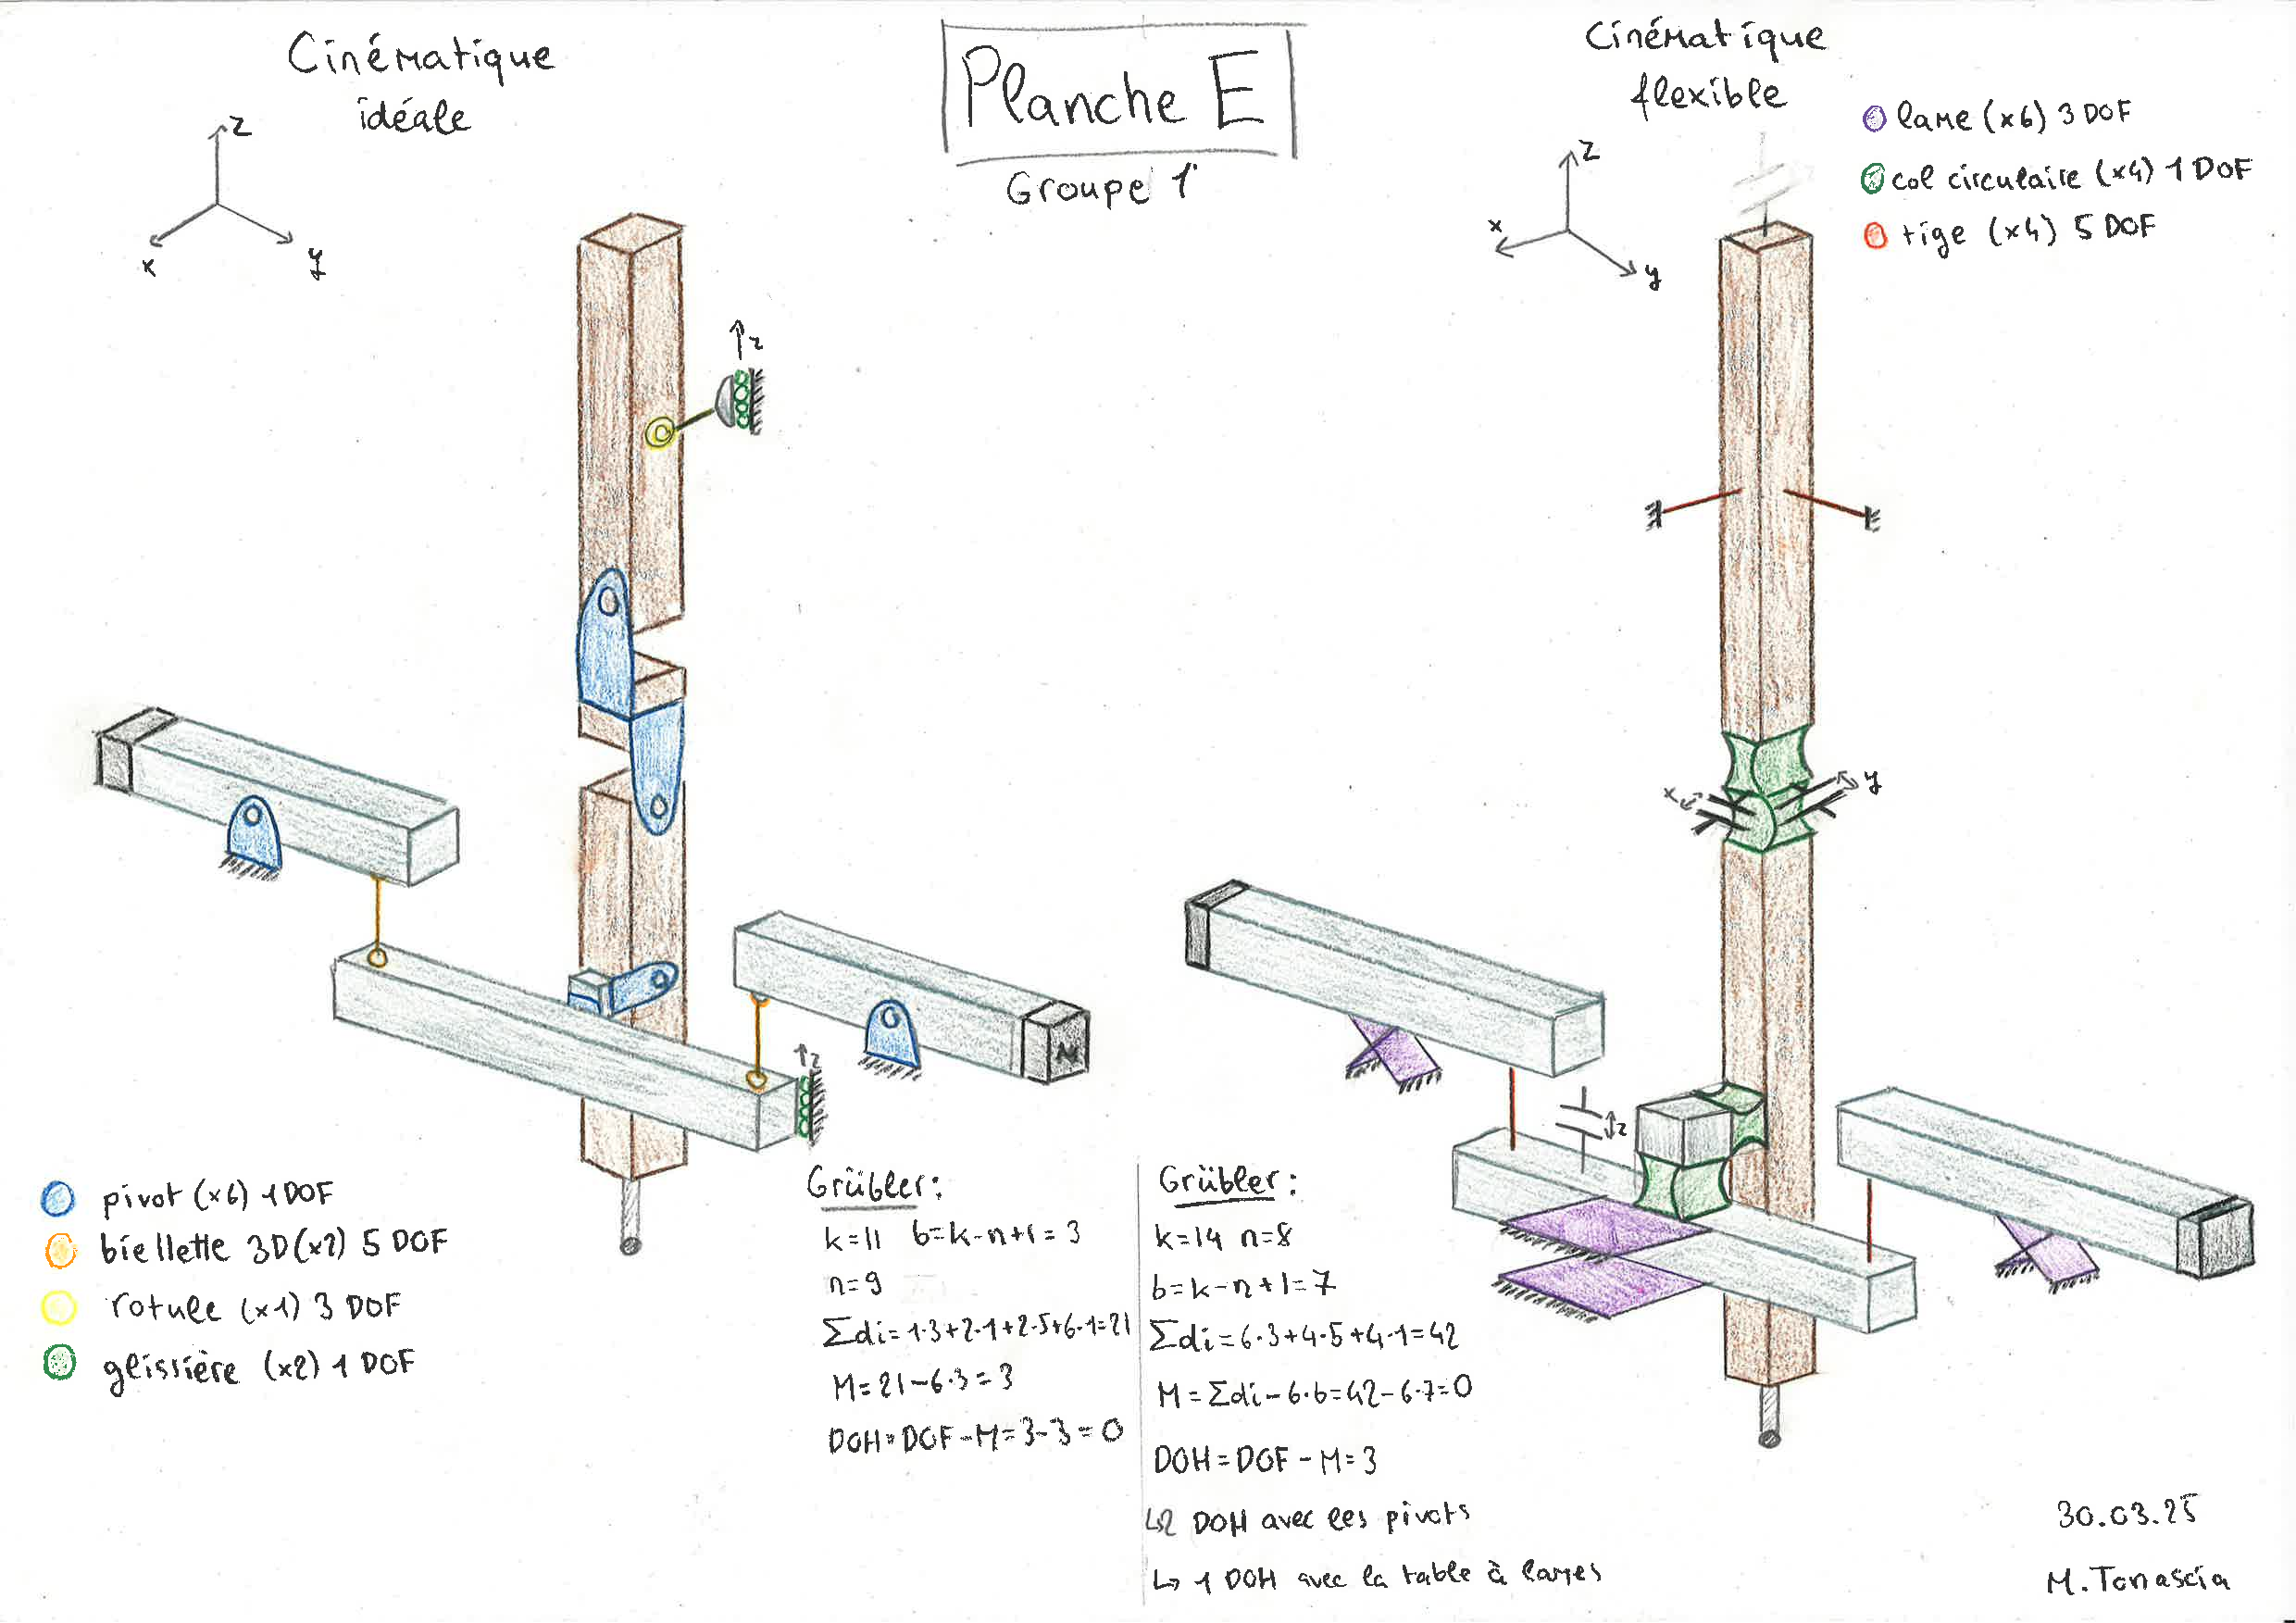
\includepdf[pages=1, landscape=true, fitpaper=true]{Annexes/G01_Planche5.pdf}
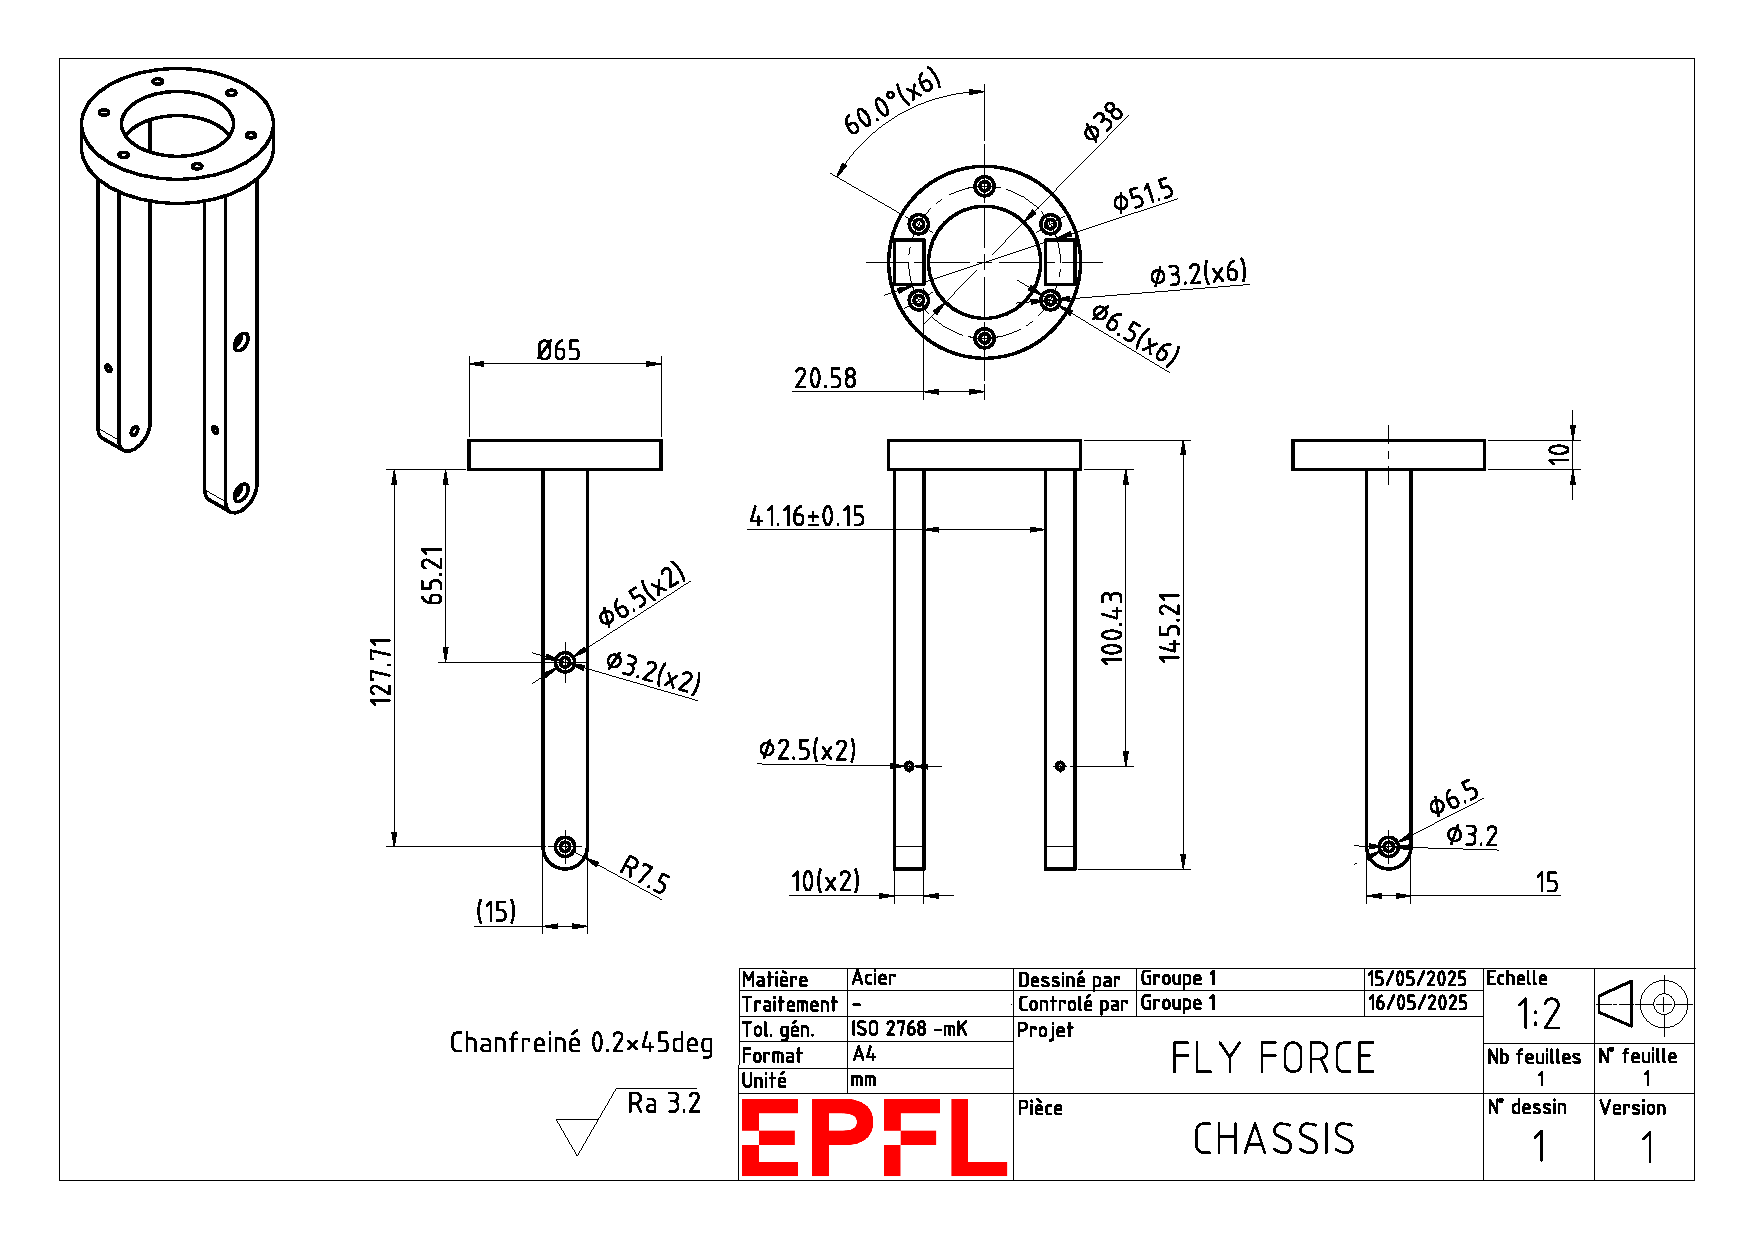
\includepdf[pages=1, landscape=true, fitpaper=true]{Annexes/CHASSIS}
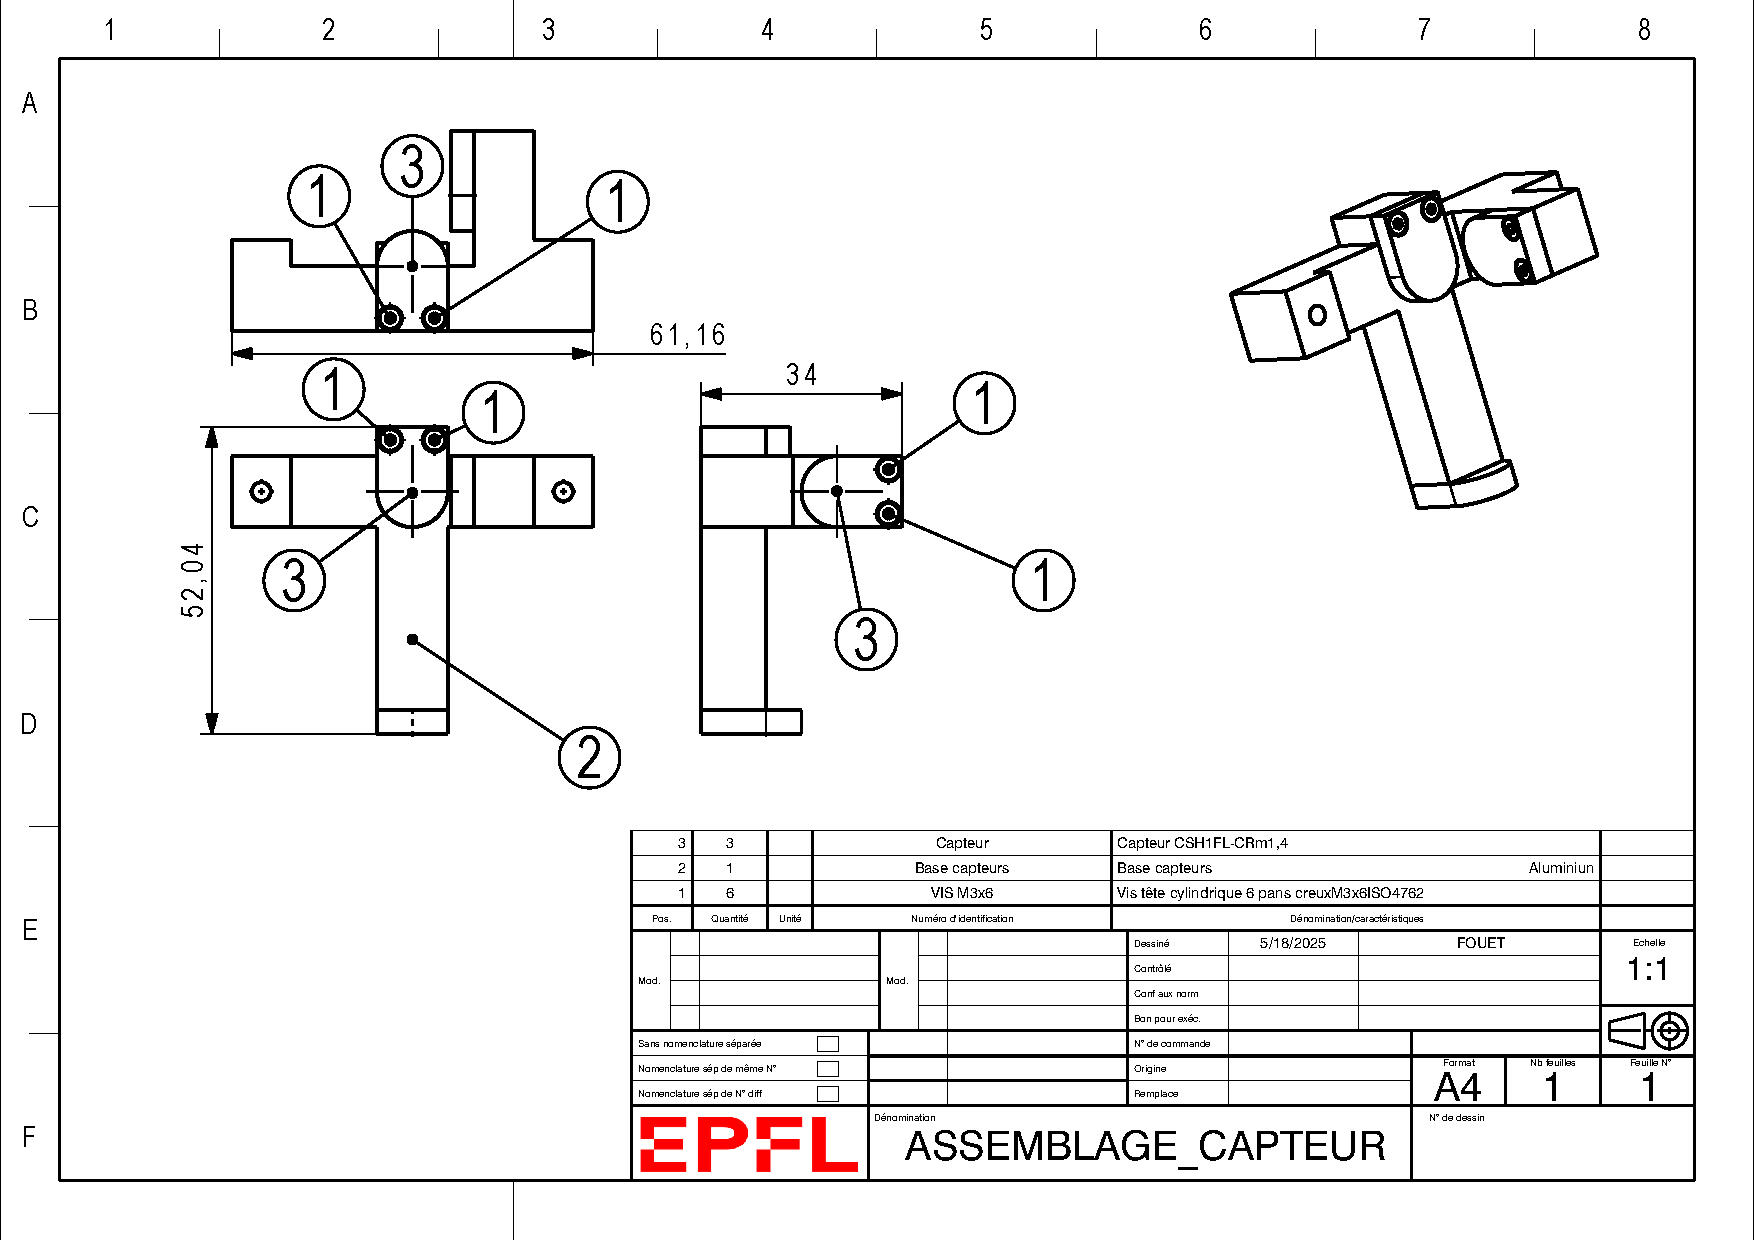
\includepdf[pages=1, landscape=true, fitpaper=true]{Annexes/ASSEMBLAGE_BASE_CAPTEUR}
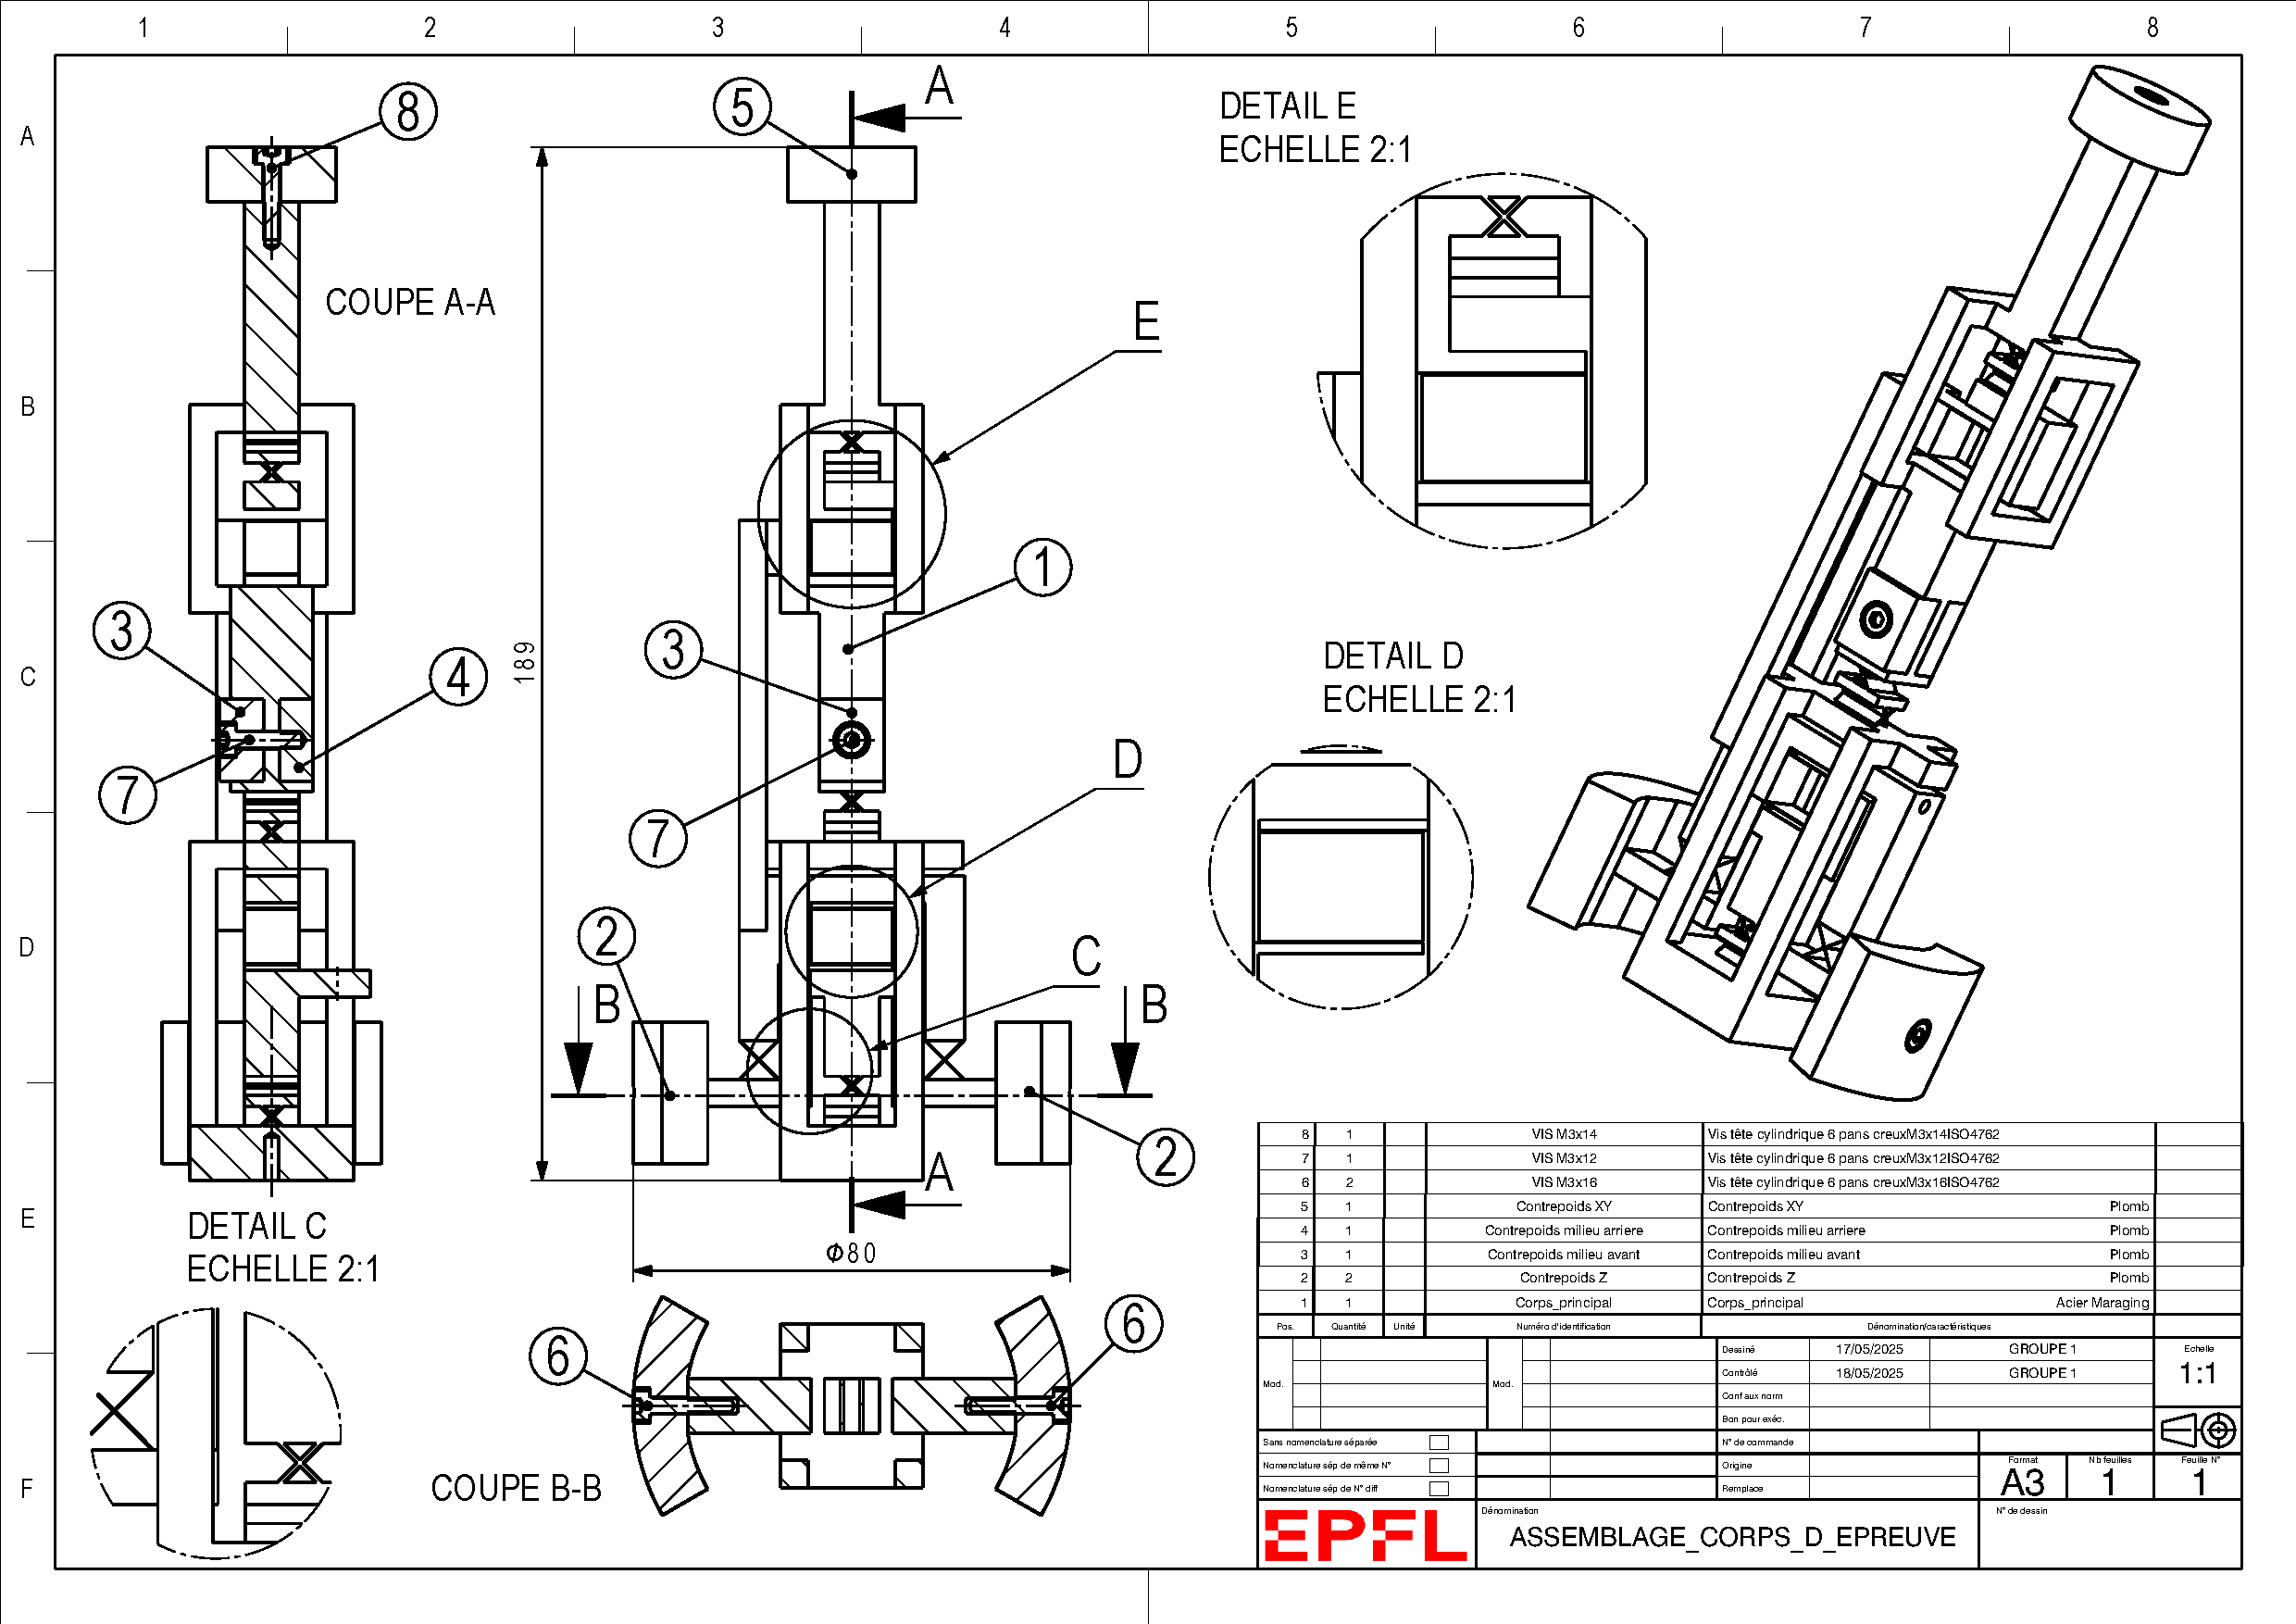
\includepdf[pages=1, landscape=true, fitpaper=true]{Annexes/CORPS_PRINCIPAL}
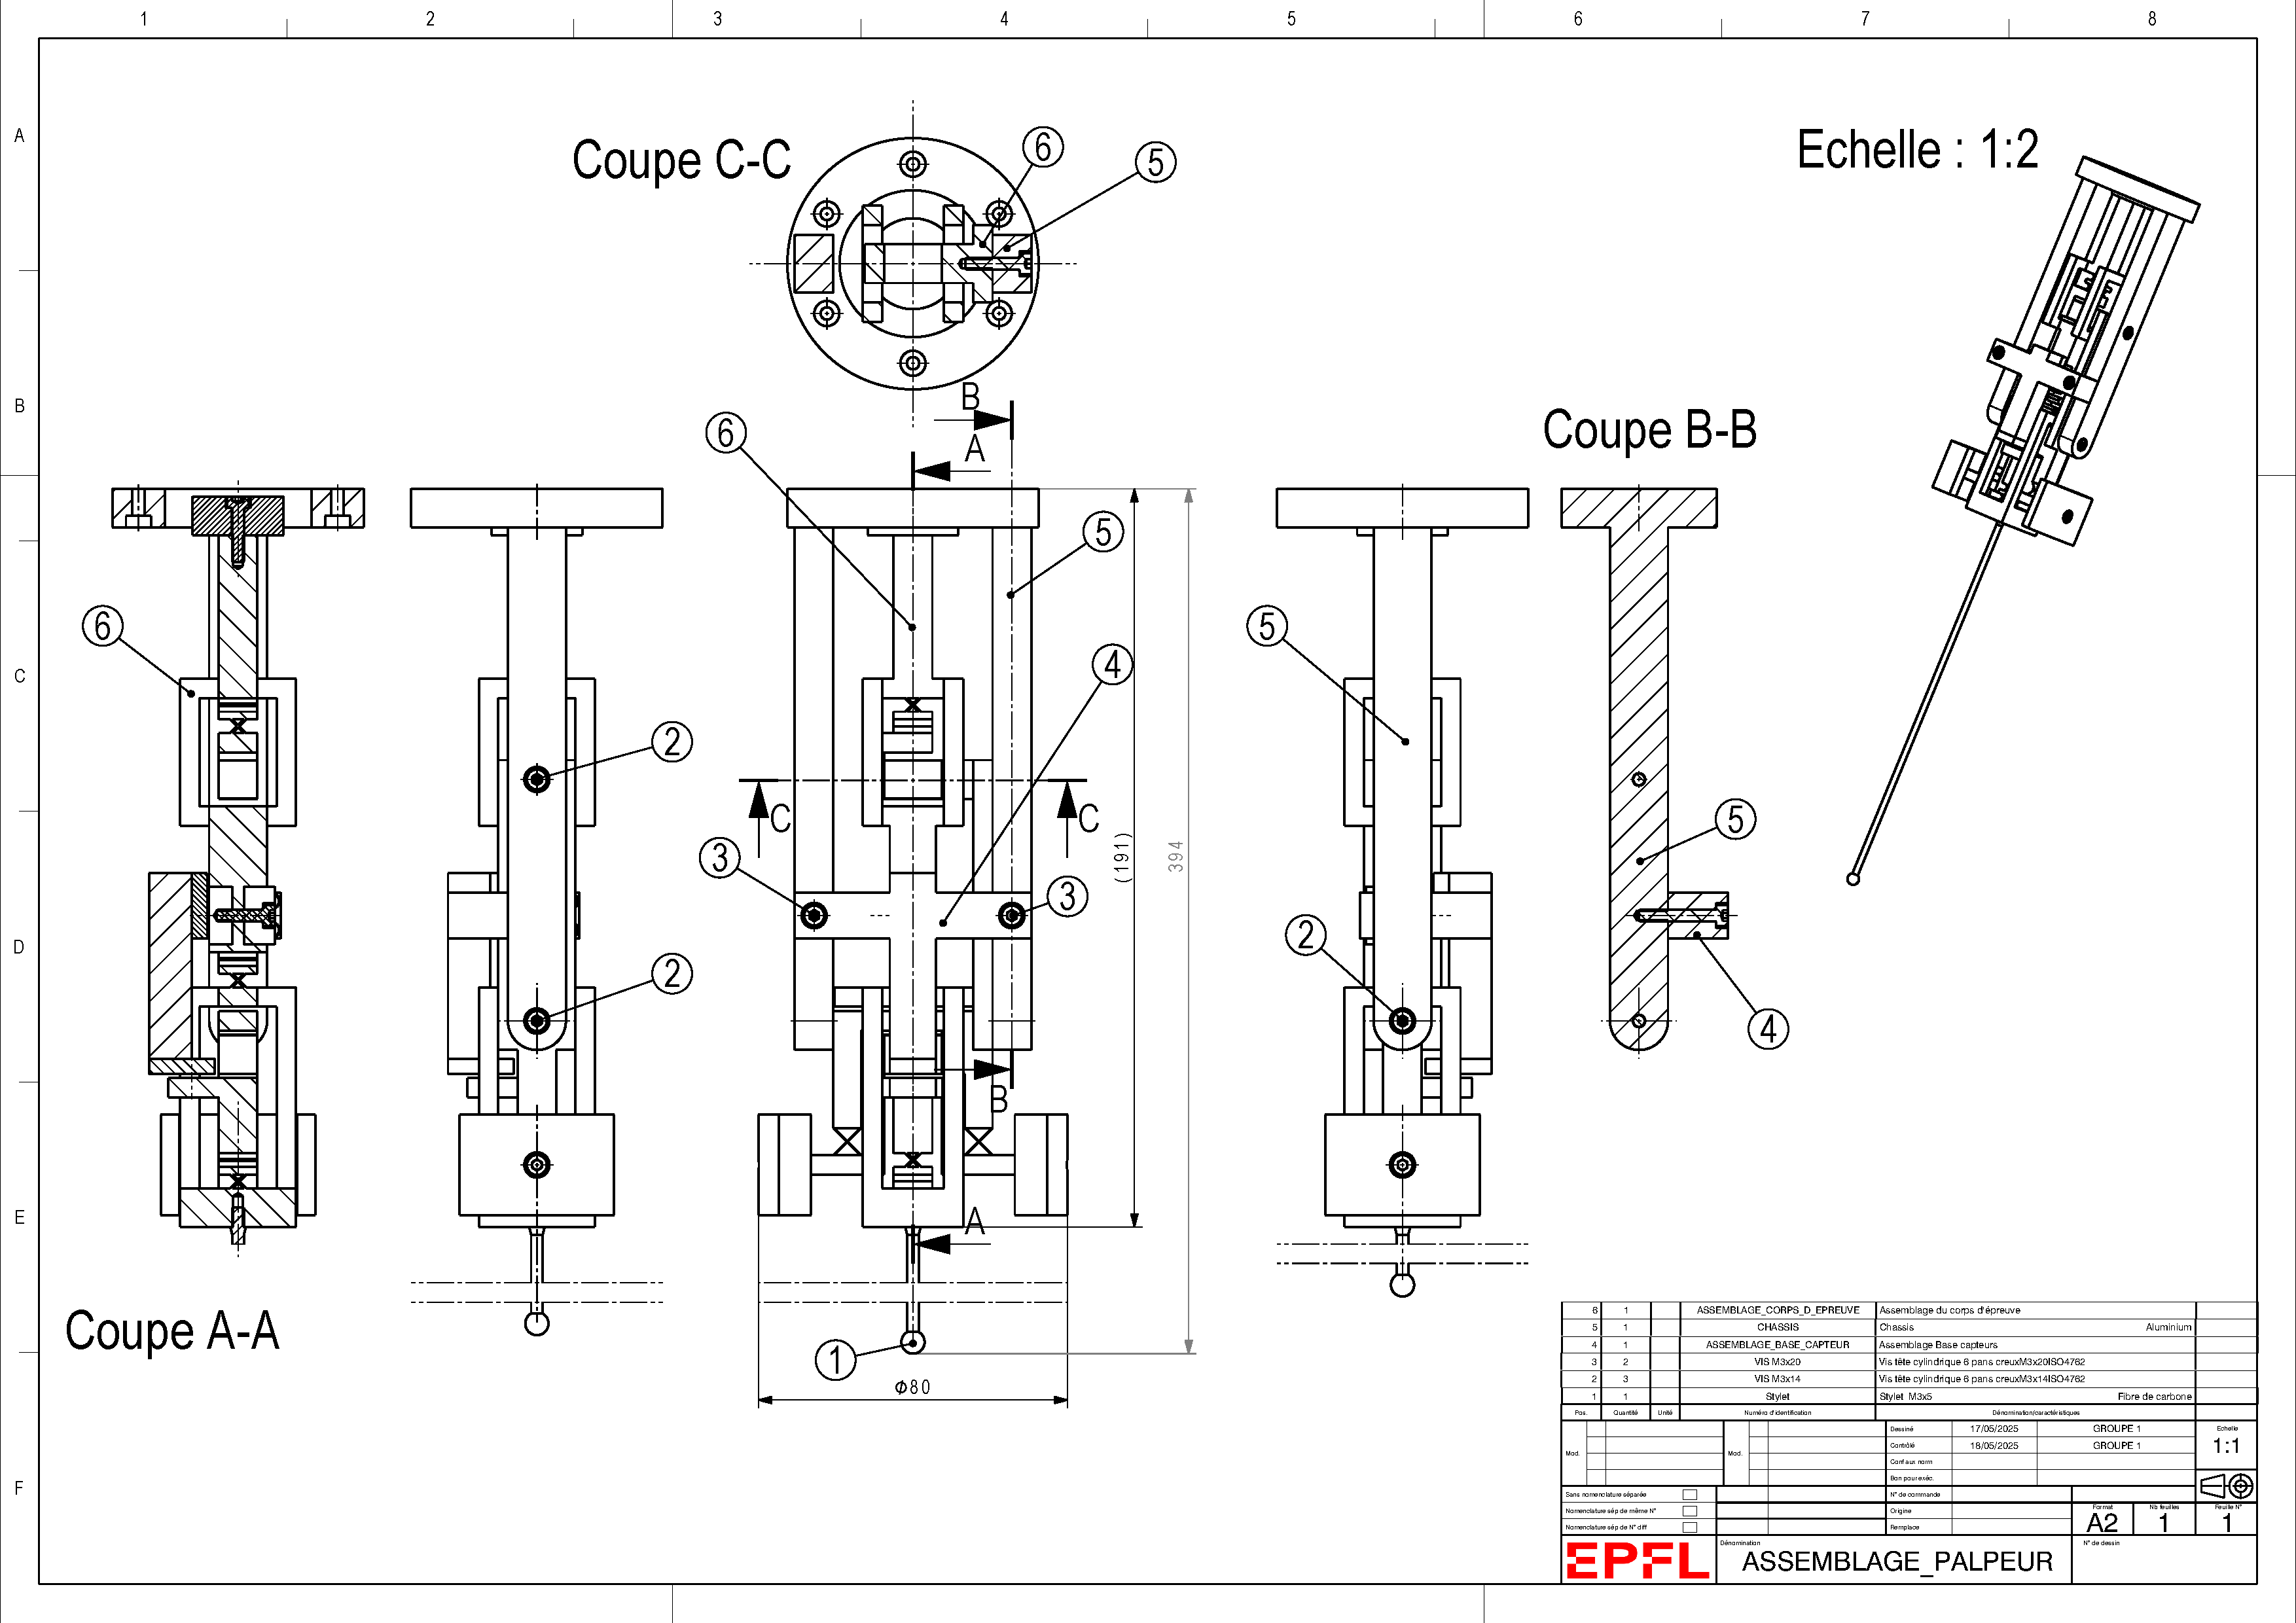
\includepdf[pages=1, landscape=true, fitpaper=true]{Annexes/ASSEMBLAGE_PALPEUR}

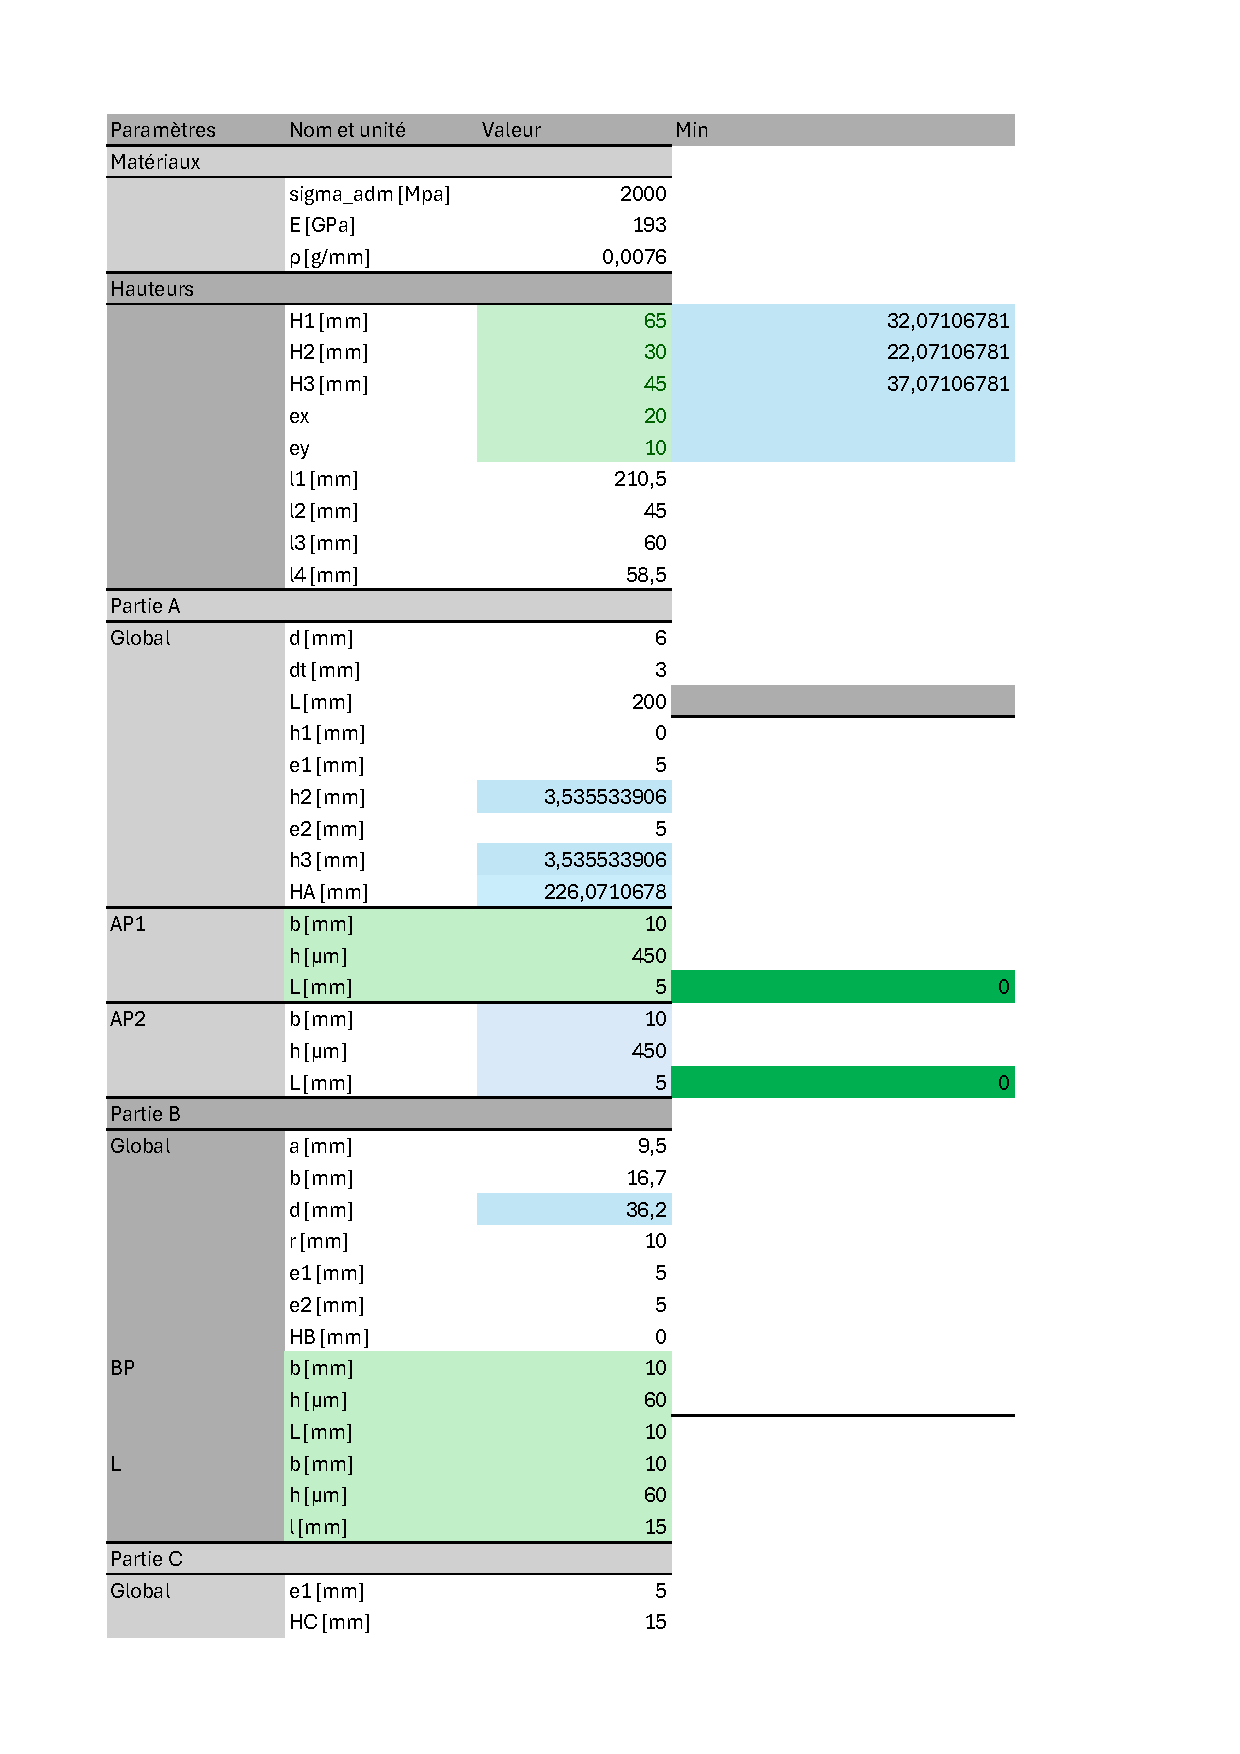
\includepdf[pages=-]{Annexes/EXCEL_PARAM.pdf}
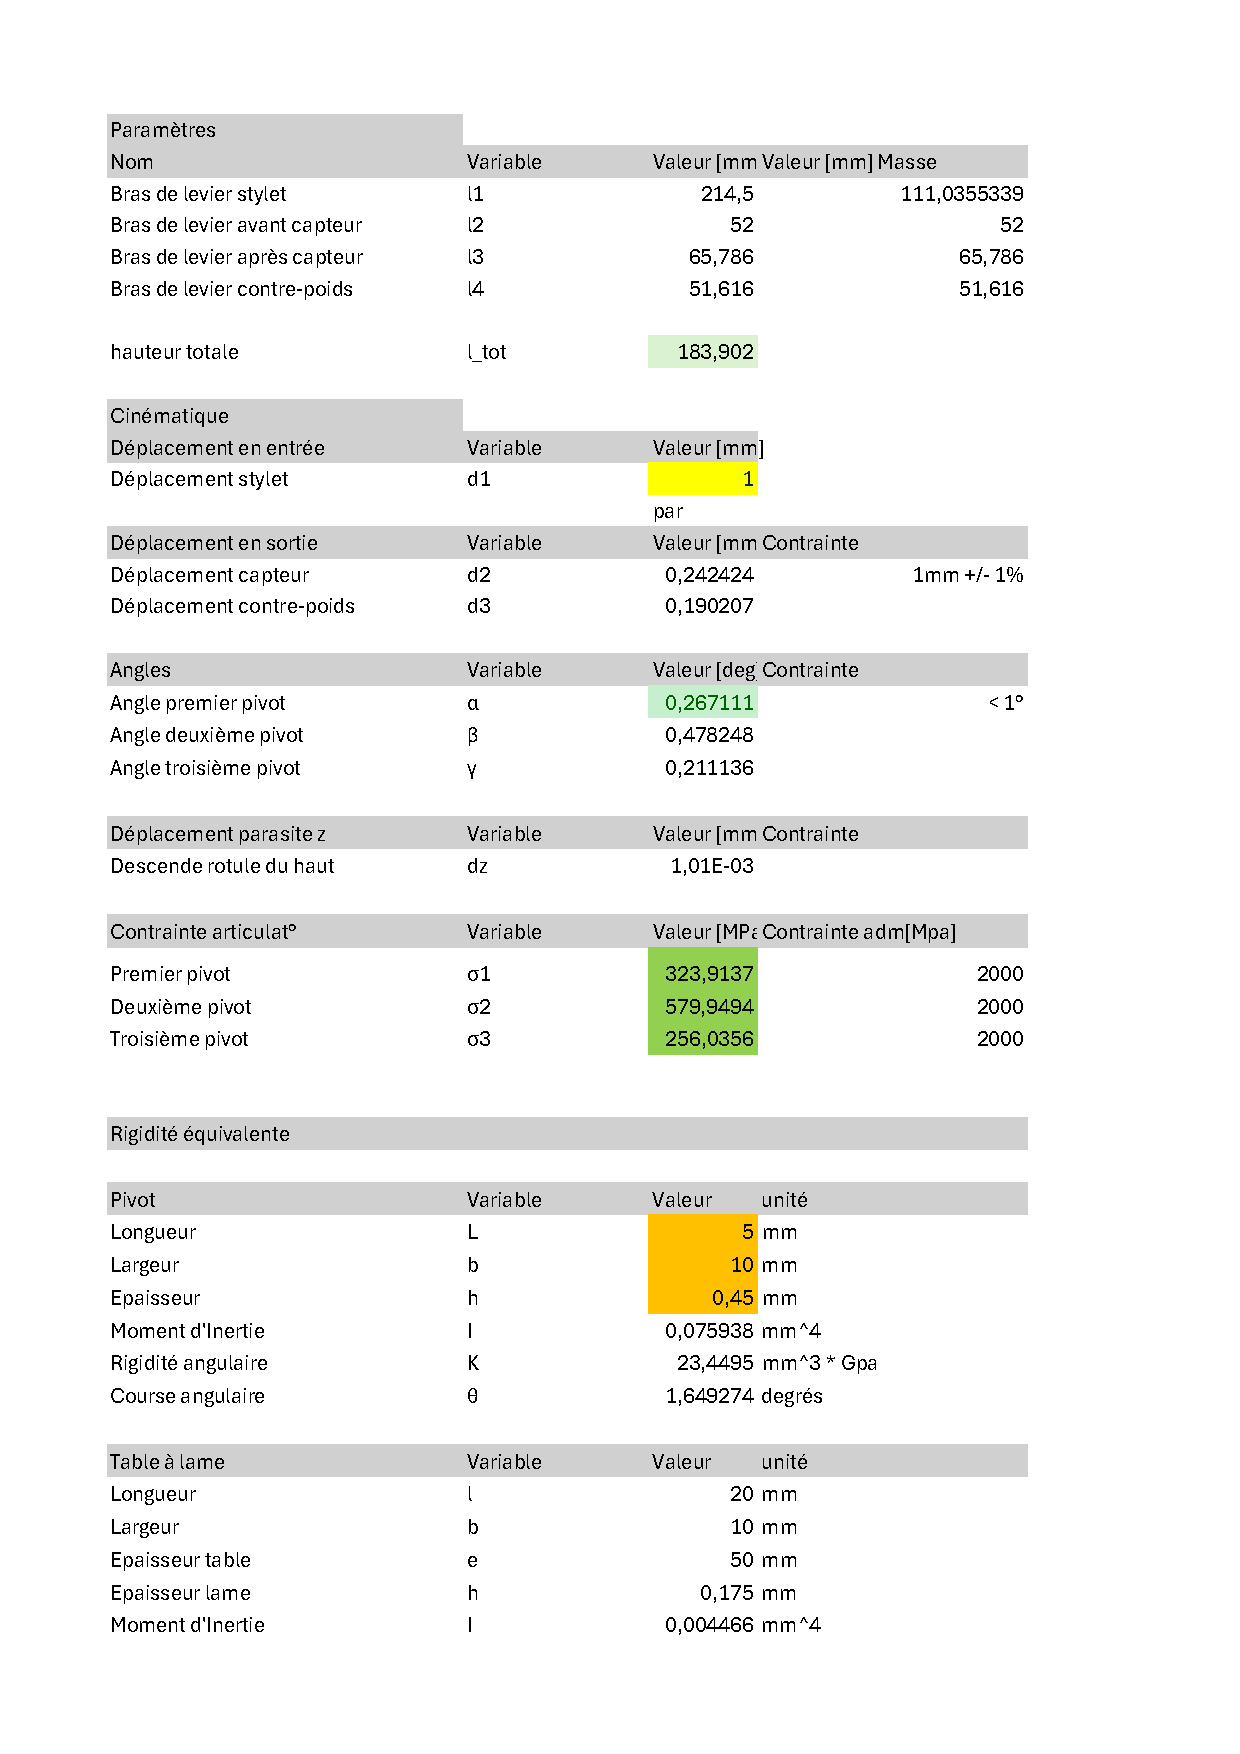
\includepdf[pages=-]{Annexes/EXCEL_AXE_XY.pdf}
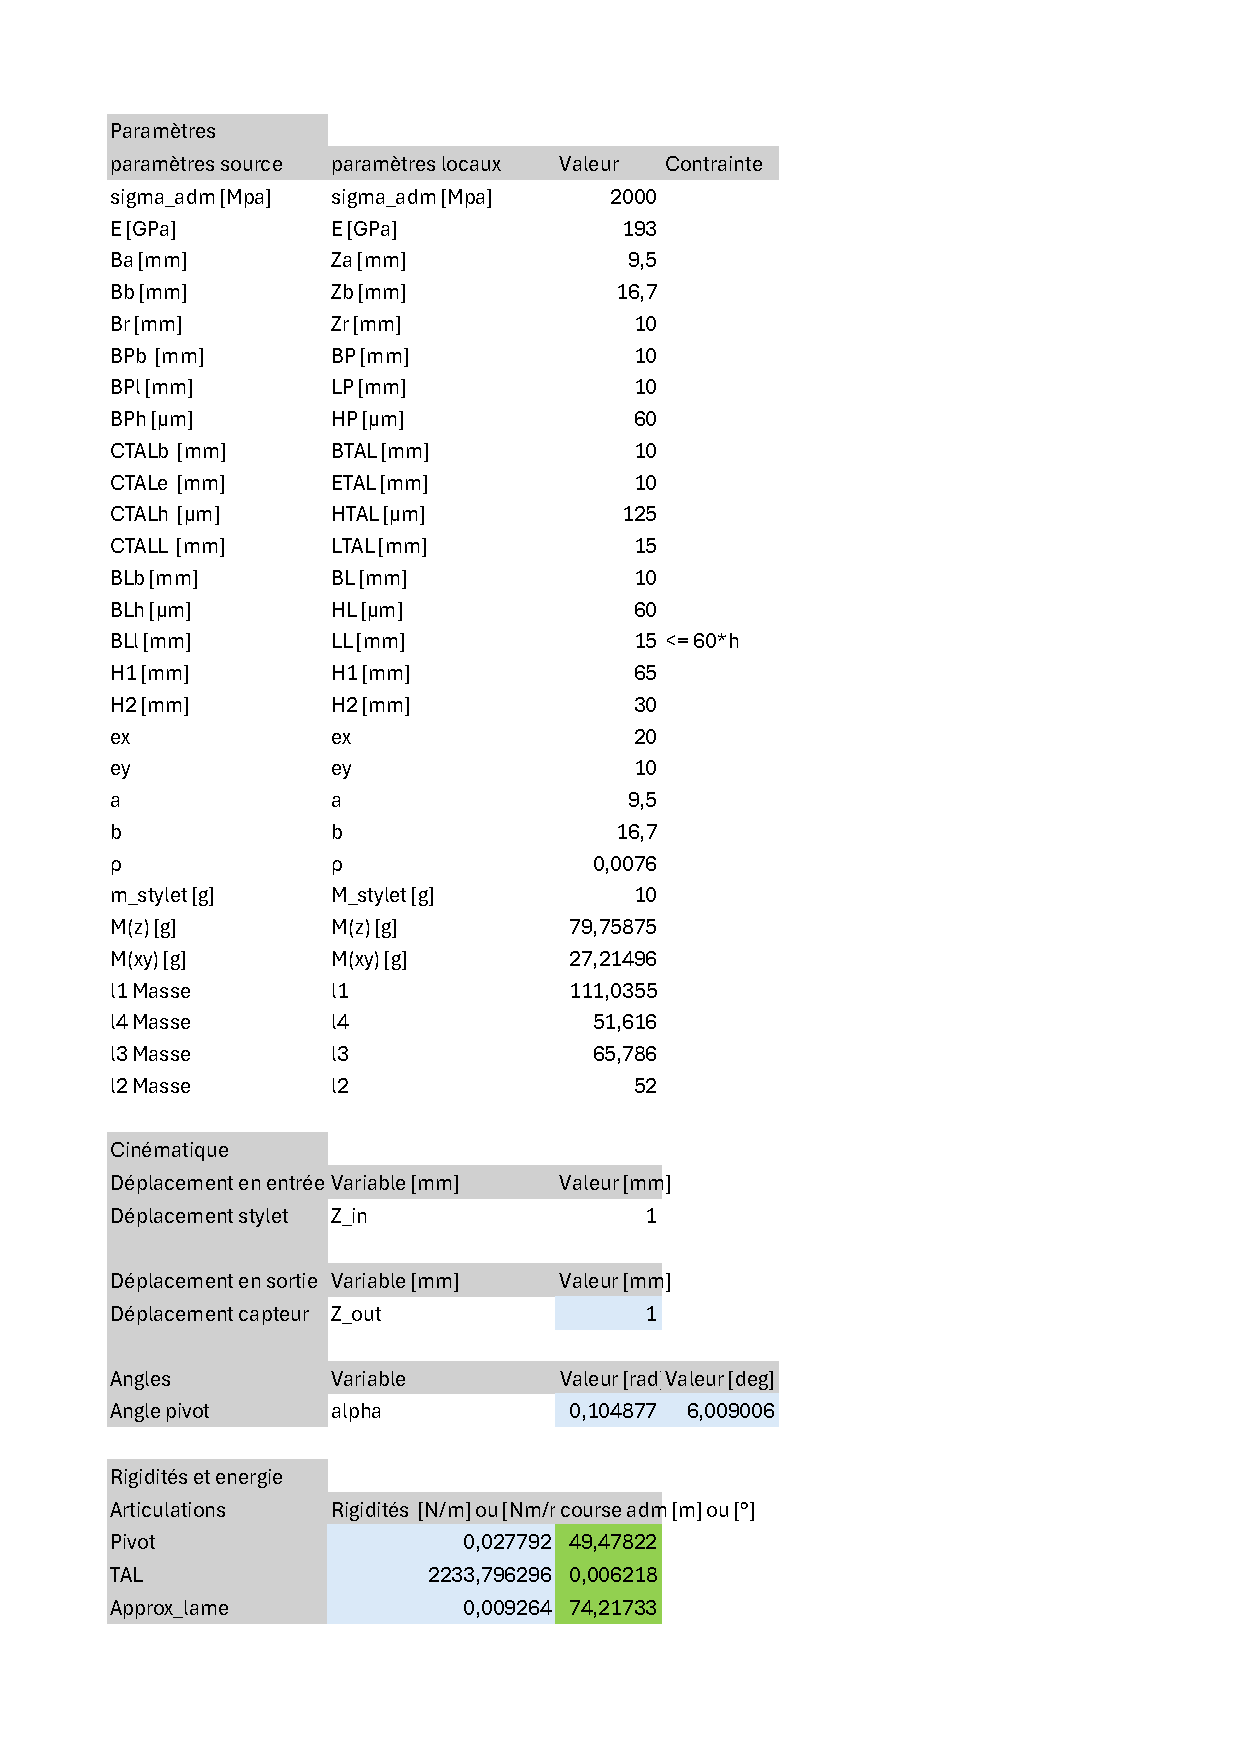
\includepdf[pages=-]{Annexes/EXCEL_AXE_Z.pdf}

\includepdf[pages=-]{Annexes/ANNEXE_CAPTEUR.pdf}

\end{document}